% techreport.tex -- Technical report for the mentor.
% Build: pdflatex techreport.tex (x2 for cross-references)
\documentclass[11pt,a4paper]{article}

\usepackage[margin=0.85in]{geometry}
\usepackage{amsmath,amssymb,amsthm}
\usepackage{mathtools}
\usepackage{pifont}
\usepackage{booktabs}
\usepackage{graphicx}
\usepackage{longtable}
\usepackage{array}
\usepackage{microtype}
\usepackage[table]{xcolor}
\usepackage{algorithm}
\usepackage{algpseudocode}
% ⟨JULIA:...⟩ placeholders (filled after the Julia reruns) use U+27E8/U+27E9.
\DeclareUnicodeCharacter{27E8}{\ensuremath{\langle}}
\DeclareUnicodeCharacter{27E9}{\ensuremath{\rangle}}
\usepackage[hidelinks,colorlinks=true,linkcolor=blue!45!black,citecolor=blue!45!black,urlcolor=blue!45!black]{hyperref}

\newtheorem{theorem}{Theorem}[section]
\newtheorem{lemma}[theorem]{Lemma}
\newtheorem{proposition}[theorem]{Proposition}
\newtheorem{corollary}[theorem]{Corollary}
\theoremstyle{definition}
\newtheorem{definition}[theorem]{Definition}
\newtheorem{remark}[theorem]{Remark}
\newtheorem{conjecture}[theorem]{Conjecture}

\newcommand{\Tmax}{\Theta_{\max}}
\newcommand{\Esplit}{E_{\mathrm{split}}}
\newcommand{\Ehinge}{E_{\mathrm{hinge}}}
\newcommand{\Eborder}{E_{\mathrm{border}}}
\newcommand{\Mprime}{M'}
\newcommand{\file}[1]{\texttt{\small #1}}
\newcommand{\POS}{\textsf{POS}}
\newcommand{\NOOV}{\textsf{NOOVERLAP}}
\newcommand{\NOROOT}{\textsf{NOROOT}}
\newcommand{\EMB}{\textsf{EMB}}
\algrenewcommand\algorithmicrequire{\textbf{Input:}}
\algrenewcommand\algorithmicensure{\textbf{Output:}}

\title{\bf Exact deployment ranges, validity certificates and range-maximising\\
embeddings for uniformly deployable kirigami\\[6pt]
\large A technical report on our extension of the Segall--Ren--Sorkine-Hornung framework}
\author{Emre Dayangaç}
\date{5 September 2026}

\setlength{\abovedisplayskip}{5pt}\setlength{\belowdisplayskip}{5pt}
\setlength{\abovedisplayshortskip}{3pt}\setlength{\belowdisplayshortskip}{3pt}
\setlength{\textfloatsep}{10pt}\setlength{\intextsep}{10pt}
\begin{document}
\maketitle

\begin{abstract}
\noindent
Segall, Ren and Sorkine-Hornung (TOG 2026) place uniformly deployable kirigami on an
arbitrary planar graph inside a linear shape space, and record as an open problem
(their Limitation~1) that membership in that space does not by itself guarantee that the
design opens without self-intersection. This report documents, in full and reproducible
detail, everything we built on top of their framework in order to answer that question.
It is a working document for a reader who wants to re-derive or re-run the work, not a
paper: every algorithm is given as pseudocode or as a pointer to the exact source file,
every number cites the file it was measured in, and every place where a claim is
measured rather than proved is tagged as such.

The content divides into four parts. First, an exact contact calculus: along the uniform
deployment branch every orientation, dot-product and squared-length predicate is a single
first harmonic $p+q\cos\theta+r\sin\theta$ whose coefficients are quadratic forms in the
flat design coordinates, so the collision-free range $\Tmax$ is computable in closed form
from a complete, finite candidate list, with grazing contacts correctly separated from
overlaps. Second, a sound sufficient validity certificate, together with an explicit
counterexample showing that it is \emph{not} complete. Third, a diagnostic campaign:
the least-norm projection of the published pipeline is certifiably non-deployable on a
population of 400 random-graph designs under four repair strategies and under the authors'
own optimiser, and the mechanism is reflex face corners introduced by the projection
itself. Fourth, a constructive replacement: keeping the framework's shape space and cut
rules exactly as published, and replacing only the objective that selects a point inside
it, makes $307$ of the same $400$ designs deployable and $306$ of them certified, against
a baseline of zero.

On $3{,}113$ designs the closed-form range agrees with a tolerance-independent bisection
referee on $3{,}113/3{,}113$ at $10^{-5}$, worst gap $3.822\times10^{-9}$, with zero
soundness violations of the certificate. All code is Julia (package \file{Kirigami}); the two test
suites re-run for this report at ⟨JULIA:tests⟩ (whole suite) and ⟨JULIA:derivation\_tests⟩ (\file{derivation\_tests.jl}), no failures.
\end{abstract}

\tableofcontents
\clearpage

%==============================================================================
\section{Purpose and reading guide}
%==============================================================================

\subsection{What this document is}

This is a technical report, not a paper. Its purpose is that every algorithmic change and
every piece of computational-geometry logic we added on top of the Segall--Ren--Sorkine-Hornung
framework is written down in enough detail to be re-derived, re-implemented and re-run by
someone who has the two papers and this repository. Where a paper would compress a
construction into a sentence, this document gives the coefficient formulas, the branch
conditions, the tolerance, the default parameter and the file and line where the code
lives.

\subsection{Relationship to the framework we extend}

Everything here is an \emph{extension} of the framework of
\begin{itemize}\itemsep2pt
\item A.\ Segall, J.\ Ren, O.\ Sorkine-Hornung, \emph{Uniformly Deployable Kirigami on
Arbitrary Planar Graphs}, ACM TOG 45(4), article 60, 2026 --- referred to throughout as
\textbf{the 2026 paper}; and
\item A.\ Segall, J.\ Ren, M.\ Padilla, O.\ Sorkine-Hornung, \emph{Reconfigurable Hinged
Kirigami Tessellations}, SIGGRAPH Asia 2025 --- \textbf{the 2025 paper}, which supplies
the hinge convention and the kinematic bound $\theta_{\max}$.
\end{itemize}
We reimplemented their pipeline from scratch, checked it against their released code at
parity, and then worked on the problem their own Limitation~1 names. Several of our
findings are corrections --- an off-by-one in a rank claim on periodic patterns, an
over-constraint in their released code, a false-negative rate in their collision test.
These are offered in the spirit in which one reports an erratum on work one has built on:
the framework is what makes all of this possible, and none of the corrections touches the
central construction of either paper. Where we measure their pipeline performing badly, it
is on a population --- random planar graphs with median face count $332.5$ --- that their
papers never claim and never demonstrate. That qualification is repeated wherever the
numbers appear, because it is load-bearing.

\subsection{How to read it}

\begin{itemize}\itemsep3pt
\item \textbf{Section~\ref{sec:framework}} restates the framework we extend, in our
notation, with the parity checks against the authors' code.
\item \textbf{Sections~\ref{sec:kinematics}--\ref{sec:certificate}} are the theory:
exact kinematics (T1, T2), the contact calculus (T3, T4), and the certificate (T5).
These are the parts a reader checking correctness should read first.
\item \textbf{Sections~\ref{sec:diagnostics}--\ref{sec:rangeembed}} are the experimental
core: what fails in the published projection and why, and the constrained
range-maximising embedding that replaces it.
\item \textbf{Sections~\ref{sec:periodic}--\ref{sec:baselines}} cover the periodic
(torus) results and the fairness of every baseline comparison.
\item \textbf{Sections~\ref{sec:software}--\ref{sec:open}} are the software map and the
honest list of what remains open, including three hostile reviews we commissioned against
our own work.
\item The \textbf{appendix} carries the full kill-test table, the dead ends and the
reproduction commands.
\end{itemize}

\subsection{Tagging convention}

The derivation files use a four-way tag that this report preserves, because it is the
only honest way to distinguish what is proved from what is merely observed:

\begin{center}
\small
\begin{tabular}{@{}ll@{}}
\toprule
tag & meaning \\
\midrule
\textbf{[D]} & a definition \\
\textbf{[F]} & a fact cited from a paper, from \file{STATE.md}, or from the code's stated convention \\
\textbf{[A]} & an algebraic step a reader can verify by hand \\
\textbf{[N]} & a numeric check that was actually run; the program is named and the result quoted \\
\bottomrule
\end{tabular}
\end{center}

\noindent A claim tagged \textbf{[N]} only is a measurement, never a theorem, and is
printed with its sample size. Claims we could not prove are marked \textsc{conjecture}
and collected in Section~\ref{sec:open}.

\subsection{Primary sources inside the repository}

\begin{center}
\small
\begin{tabular}{@{}ll@{}}
\toprule
content & file \\
\midrule
the derivation, six deriver/checker rounds & \file{derivations/core.md} \\
the independent checker's rebuttals and tests & \file{derivations/check.md} \\
every experiment, its bar and its verdict & \file{results/kill/KILL\_REPORT.md} \\
the 3{,}113-design validation & \file{results/final/e1/E1.md} \\
API, JSON contract, 16 judgement calls & \file{code/README.md} \\
facts F1--F40, decisions D1--D11, dead ends & \file{STATE.md} \\
the three hostile reviews & \file{review/\{theory,negative,constructive\}\_review.md} \\
notes on the two papers, equation by equation & \file{notes/paper\_2026.md}, \file{notes/paper\_2025.md} \\
\bottomrule
\end{tabular}
\end{center}

\clearpage
%==============================================================================
\section{The framework we extend}
\label{sec:framework}
%==============================================================================

This section restates the 2026 pipeline in the notation used for the rest of the report,
records the places where the published description is silent or incomplete and what we
chose instead, and reports the parity of our reimplementation against the authors' released
code.

\subsection{Cut rules: the orientation \texorpdfstring{$\sigma$}{sigma} and the two cut types}

\textbf{[D]} $M=(V,E,F)$ is a straight-line embedded planar graph, $N=|V|$, with vertex
positions $X\in\mathbb{R}^{N\times2}$ (row $x_v$) and faces stored counter-clockwise in the
given geometry.

\textbf{[F, 2026 §3]} A face-orientation assignment is a map $\sigma:F\to\{-1,+1\}$, where
$\sigma(f)=+1$ means face $f$ is traversed \emph{clockwise}. This induces a direction on
each half-edge. The interior edges split into two classes:
\[
E \;=\; \Eborder \;\sqcup\; \Ehinge \;\sqcup\; \Esplit ,
\]
where an interior edge shared by $f_1,f_2$ is a \textbf{hinge cut} when
$\sigma(f_1)=-\sigma(f_2)$ and a \textbf{split cut} when $\sigma(f_1)=\sigma(f_2)$.

The distinction is the whole mechanism. At a hinge edge the two $\sigma$-induced half-edge
directions agree, giving the edge a direction $\mathrm{src}(e)\to\mathrm{dst}(e)$; the cut
\emph{keeps the two faces pinned at the source vertex} and duplicates the target. At a
split edge the two half-edge directions are antiparallel, no pin is formed, and both
endpoints are duplicated.

\begin{center}
\small
\begin{tabular}{@{}p{0.46\textwidth}p{0.46\textwidth}@{}}
\toprule
\textbf{hinge cut} ($\sigma(f_1)=-\sigma(f_2)$) & \textbf{split cut} ($\sigma(f_1)=\sigma(f_2)$)\\
\midrule
both half-edges point $v_i\to v_j$ &
half-edges are antiparallel \\
the pin \emph{stays at the source} $v_i$ &
both endpoints are duplicated \\
the target $v_j$ is duplicated &
no pin is formed \\
opens by exactly $\theta$ (Sec.~\ref{sec:kinematics}) &
duplicates stay equal translates (T1.B) \\
\bottomrule
\end{tabular}
\end{center}

\noindent
\textbf{A convention worth stating twice.} Our first implementation put the hinge at the
\emph{target}; the 2026 paper §3 and the 2025 paper §3.1 both say \emph{source}, and the
Builder caught the discrepancy against the papers' own figures. Every formula in this
report is in the source convention (\file{STATE.md} F1). Flipping it is not a relabelling:
$\sigma\mapsto-\sigma$ globally also reverses every hinge direction and therefore produces
a different cut structure.

Two consequences that we assert everywhere in the code:
\begin{itemize}\itemsep2pt
\item \textbf{[F, 2026 Remark A.1]} At every interior vertex the number of hinge edges
directed \emph{in} equals the number directed \emph{out}. Verified on 250 random
$(\text{graph},\sigma)$ pairs in \file{kiri\_tests}.
\item \textbf{[F, 2026 Remark A.4]} The two duplicates of a split edge stay parallel
throughout deployment. In our formulation this is one line (Lemma~\ref{lem:t1b}) rather
than the induction over the split forest that 2026 Appendix~A gives.
\end{itemize}

\subsection{Choosing \texorpdfstring{$\sigma$}{sigma}: Eq.~(2026-1)}

\textbf{[F, 2026 §4.2, Eq.~(1)]} The paper chooses $\sigma$ by an approximate max-cut on the
dual graph $M_d$, minimising $\sum_{(i,j)\in E_d} x_i\!\cdot\!x_j$ subject to $\|x_i\|=1$,
then splitting the circle by a diameter. Maximising the cut minimises $|\Esplit|$, which is
the paper's stated goal (``many balanced, small holes''), under two principles: (1) $\Mprime$
stays connected, (2) holes stay local and small.

\textbf{Judgement call 8 (\file{code/README.md}).} The rounding is unspecified in the paper
--- ``a diameter then partitions the circle'' names no randomisation, repetition count or
selection rule. We implement projected gradient descent on the unit circle with random
restarts, then take the best of 180 evenly spaced diameters, ranked first by the number of
connected components of $\Mprime$ (the paper's principle 1) and then by $|\Esplit|$
(principle 2). Two repairs are applied to each candidate: flip any face whose dual
neighbours all share its orientation, and flip a boundary face of the smallest component
while $\Mprime$ is disconnected. \textbf{[N]} This gives $c(\Gamma)=1$ on 50/50 sweep graphs.

We also carry a second orientation rule, $\sigma_{\mathrm{def}}$, introduced in
Section~\ref{sec:diagnostics}: a greedy local search minimising the deployability defect at
the input embedding. It is not from the paper; it is one of the design variables we tested.

\subsection{Hole preimages and Algorithm 1}

\textbf{[F, 2026 Def.~4.1--4.2, Alg.~1]} A \emph{hole} is a bounded region of $\Mprime$
opened by the cuts; its \emph{preimage} $C$ is the set of edges of $M$ whose duplicates
bound it. Algorithm~1 grows a preimage from a seed hinge edge under three adjacency rules
stated in prose: split--split edges are always in the same preimage; hinge--hinge edges are
in the same preimage iff both point at the shared vertex; hinge--split edges are in the same
preimage iff the hinge points at the shared vertex.

\textbf{Judgement call 1: Algorithm 1 line 10 is incomplete.} The pseudocode tests only that
the \emph{candidate} hinge edge points at the shared vertex, and never that $e'$ does, so as
written it does not implement the stated hinge--hinge rule. We implement the prose rules
instead: for a hinge edge only its \emph{target} is a growth vertex; for a split edge both
endpoints are. \textbf{[N]} With that reading Algorithm~1 becomes provably identical to a
much simpler formulation, which is what the code actually uses:

\begin{proposition}[the split-forest partition, \file{STATE.md} F11]
\label{prop:f11}
Let $S$ be the split-edge subgraph of $M$, and let its connected components be $K$ (an
interior vertex touched by no split edge is a trivial component). Then the hole preimages
are exactly
\[
C_K \;=\; E(K)\;\cup\;\{\, e\in\Ehinge : \mathrm{dst}(e)\in V(K) \,\}.
\]
In particular the preimages \textbf{partition} $\Ehinge\sqcup\Esplit$, and in the pure case
$\Esplit=\varnothing$ there is one hole per interior vertex, $C_v=\{\text{in-edges of }v\}$.
\end{proposition}

\noindent
\textbf{[N]} Three independent constructions are cross-checked on every test graph:
\file{holes\_seed\_growing} (Algorithm~1 with the prose rules), \file{holes\_partition}
(Proposition~\ref{prop:f11}), and \file{holes\_geometric} (tracing the bounded complement
components of the deployed $\Mprime$ as a planar arrangement). They agree on 100/100 sweep
graphs, and --- the stronger test --- on \textbf{398/398} pairs with a \emph{fully random}
$\sigma$, among them 334 with $c(\Gamma)>1$ and 210 with split-cut cycles
(\file{derivations/check.md}, check CE-a).

\textbf{Judgement call 2: which preimages become rows.} The paper never says what happens to
a preimage that runs into the mesh boundary. Measured answer: the preimages whose vertex set
is entirely interior are exactly the bounded holes of Definition~4.1, and only those
contribute rows. Preimages touching the boundary are \emph{notches} open to the exterior.
\textbf{[N]} $H = |\Ehinge| - |F| + c(\Gamma)$ holds on 50/50 sweep graphs and 8/8 reference
cases when $H$ counts holes only; including the notches breaks it on 0/50.

\subsection{Eq.~(2): the deployability condition}

\textbf{[F, 2026 Prop.~4.1, Eq.~(2)]} A kirigami structure $\Mprime$ is \emph{uniformly
deployable} if and only if, for every hole preimage $C$,
\begin{equation}
\sum_{e\in C\cap\Ehinge} \bigl(x_{\mathrm{dst}(e)}-x_{\mathrm{src}(e)}\bigr) \;=\; 0 ,
\tag{2026-2}
\label{eq:eq2}
\end{equation}
the sum of the \emph{directed} hinge-edge vectors of the preimage. Split-cut edges do not
appear. \textbf{[F, 2026 Remark 4.1]} The condition is affine-invariant.

The paper's proof of Prop.~4.1 reduces the hole to a $2k$-gon with paired edge lengths and
all hinge angles equal to $\theta$, and then delegates the closure step to Appendix~B of the
2025 paper. Section~\ref{sec:kinematics} re-derives the same condition from the kinematics
directly, as the closure of a discrete 1-form on the hinge graph, which is what makes the
downstream calculus possible.

\subsection{Eq.~(4): the linear system; Eq.~(5): the shape space; Eq.~(6): the projection}

\textbf{[F, 2026 Eqs.~(3)--(6)]} Assembling \eqref{eq:eq2} over all $H$ hole preimages plus
boundary conditions gives
\begin{equation}
\begin{bmatrix} L_{H\times N}\\ B_{B\times N}\end{bmatrix} X_{N\times2}
\;=\;
\begin{bmatrix} 0_{H\times2}\\ T_{B\times2}\end{bmatrix},
\tag{2026-4}
\label{eq:eq4}
\end{equation}
where each row of $L$ carries $\pm1$ entries on the endpoints of the hinge edges of one
preimage, and $B,T$ encode either fixed boundary positions or the periodic identifications
$x_p-x_{p'}=t_h$, $x_q-x_{q'}=t_v$ of Eqs.~(3b)--(3c). The solution set is the
\textbf{shape space}
\begin{equation}
\mathbb{X} \;=\; \Bigl\{\, X_0+\textstyle\sum_i \phi_i\, t_{\phi_i}^{\!\top} \,\Bigr\},
\qquad t_{\phi_i}\in\mathbb{R}^2,
\tag{2026-5}
\label{eq:eq5}
\end{equation}
with $\{\phi_i\}$ the null-space basis of the system matrix from an SVD. Each $\phi_i$
contributes \emph{two} real degrees of freedom, an $x$- and a $y$-offset. Throughout this
report we write $X(t)=X_0+\Phi t$ with design coordinates $t\in\mathbb{R}^{k\times2}$, and
$k=\dim\mathrm{null}$.

The particular solution used in practice is the least-norm projection
\begin{equation}
X_0 \;=\; \arg\min_X \|X-X^{\mathrm{ini}}\|^2 \quad\text{s.t.\ \eqref{eq:eq4}} .
\tag{2026-6}
\label{eq:eq6}
\end{equation}
This is the ``repair a non-auxetic tiling'' operation and the object almost all of our
diagnostic work is about.

\textbf{[N] Measured structure of the shape space.} $\dim\mathrm{null} = V_{\mathrm{int}}-H
= |\Esplit|$ on 100/100 random graphs with a fixed boundary, and $\mathrm{rank}(L)=H$ on
100/100 --- a sharper statement than the paper's ``otherwise the system becomes
rank-deficient''. Shape spaces on random graphs are large: $\dim\mathrm{null}$ reaches 1017
on a 1052-face Voronoi patch, so optimisation inside the null space is not a vacuous idea
(\file{STATE.md} F19).

\textbf{Judgement calls 4, 5, 11.} The paper gives no numerical rank threshold; we use
$\sigma_i > \max(10^{-10}\sigma_{\max},10^{-14})\cdot\max(\text{rows},\text{cols})$. Dense
SVD is used up to $N\le1400$ and \file{SparseQR} with pivot threshold $10^{-9}$ above that
--- with the caveat, measured in Section~\ref{sec:baselines}, that \file{SparseQR} ranks
above roughly 700 columns are unreliable and must not be quoted. Periodic boundaries are
imposed as linear constraints on a finite patch whose boundary edges are \emph{not}
topologically identified; Section~\ref{sec:periodic} explains why that is not good enough
for the periodic Jacobian and builds the genuine torus quotient instead.

\subsection{Eq.~(9): the collision-prevention step}

\textbf{[F, 2026 Eqs.~(7)--(9)]} The paper's collision handling is a penalty solved at
$\theta=0$. With $z_i$ the $i$-th row of $\partial g(Y^\theta,\alpha)/\partial\alpha|_{\alpha=0}$
--- the infinitesimal displacement of vertex $v_i$ under further opening --- it minimises
\begin{equation}
\min_{Y\in\mathbb{X}} \;\sum_{(v_i,v_j)\in\Esplit}
B\!\left( z_i(Y)\cdot\Bigl(\tfrac{y_i-y_j}{\|y_i-y_j\|}\Bigr)^{\!\perp}\right)
\;+\;\gamma\,\|Y-Y^0\| .
\tag{2026-9}
\label{eq:eq9}
\end{equation}

\textbf{Judgement calls 6, 7.} The barrier $B$ is described (``high penalty to negative
values, vanishing for positive'') but never given a formula; we use
$B(s)=\kappa\log(1+e^{-s/\kappa})$ with $\kappa=0.05$. The regulariser weight $\gamma$ is
never given a value, and we measured that a single $\gamma$ can make $\theta_{\max}$
\emph{worse}, because the objective contains no term that keeps the flat embedding embedded.
Our \file{optimize\_collision\_sweep} therefore runs a ladder
$\gamma\in\{10^{-4},10^{-3},10^{-2},3\!\cdot\!10^{-2},10^{-1},3\!\cdot\!10^{-1},1,3,10\}$ and
keeps the best, with $T=0$ as a fallback. We square the regulariser, following Eqs.~(6) and
(13), rather than leaving it unsquared as Eq.~(9) prints it.

\textbf{An important withdrawal.} An early finding of ours --- that Eq.~(9) ``achieves
nothing'' on the snub-square pattern --- was measured against \emph{our} reimplementation of
Eq.~(9) and is \textbf{withdrawn}. Against the authors' native \file{prevent\_intersections}
at published defaults (barrier $0.1$, strength $10$, close $0.1$), the snub square reaches
$\theta_{\max}=\pi$, certified by our own bisection, and the 4.8.8 pattern reaches $2.354$
(\file{STATE.md} F18). Our Eq.~(9) reimplementation is the weakest of the three
implementations we have and is never used as a baseline for anything. Any margin claim in
this report is against \emph{their} code.

Section~\ref{sec:certificate} makes precise what Eq.~(9) does and does not certify: it
tests the first-order separation $h'(0)$ of a split-edge pair and is blind by construction
to the second-order coefficient that decides whether the pair re-closes later.

\subsection{Our reimplementation, and parity with the authors' code}

The reimplementation is a Julia package (\file{Kirigami}, Julia $\geq 1.10$) on the standard library
(\file{LinearAlgebra}, \file{SparseArrays}, \file{Random}, \file{Statistics}) plus \file{StaticArrays}, \file{JSON}
and \file{DelaunayTriangulation}; no external optimiser --- the L-BFGS with backtracking line search in
\file{core/optimize.jl} is ours. The library layout is in Section~\ref{sec:software}.

\textbf{Parity (\file{baseline/parity.md}).} We build the authors' code natively
(\file{baseline/native}, libigl 2.5, Optiz, Eigen 3.4 via FetchContent, their \file{bind.cpp}
replaced by a CLI) and compare on 8 reference graphs:

\begin{center}
\small
\begin{tabular}{@{}lc@{}}
\toprule
check & agreement \\
\midrule
$\Ehinge$ and $\Esplit$ agree exactly as sets & 8/8, symmetric difference 0 \\
their $X_0$ satisfies our Eq.~\eqref{eq:eq4} & $4\times10^{-15}$ \\
their $X_0$ satisfies their own system & $6\times10^{-15}$ \\
forward kinematics at $30^\circ$, both codes, on a deployable embedding & $\le 4\times10^{-8}$, 8/8 \\
\bottomrule
\end{tabular}
\end{center}

\subsubsection*{F23: their extra boundary-component row is an over-constraint}

\textbf{[F, \file{STATE.md} F23]} Their code adds a constraint row for split-forest
components that \emph{touch the mesh boundary}; we drop those as notches (judgement call 2).
Consequently their $X_0$ satisfies our system on 8/8, while our $X_0$ has residual $1.73$
(hexagons) and $1.00$ (snub square) in theirs, and our null space is one dimension larger on
those two patterns.

The reasoning is that the faces around a boundary-touching component form a \emph{path} in
the hinge graph $\Gamma$ --- the exterior breaks the cycle --- so no closure constraint is
needed there. We tested this by forward kinematics, and the check run was stronger than the
one asked for: not two seed faces but \emph{every} seed face, plus 20 randomised BFS visit
orders, at four angles.

\begin{center}
\small
\begin{tabular}{@{}lrrrrr@{}}
\toprule
pattern & $|F|$ & seeds & orders & worst seed disagreement & worst hinge-angle error \\
\midrule
\file{hexagons\_auto} & 10 & 10 & 20 & $2.23\times10^{-15}$ & $6.66\times10^{-16}$ \\
\file{snub\_square\_33434} & 53 & 53 & 20 & $7.16\times10^{-15}$ & $3.55\times10^{-15}$ \\
\bottomrule
\end{tabular}
\end{center}

\noindent
\textbf{[N]} Worst over both patterns and all four angles: seed/order disagreement
$7.161\times10^{-15}$, hinge-angle error $3.553\times10^{-15}$, split-duplicate parallel
error $9.295\times10^{-16}$ --- all far inside the $10^{-9}$ the check asks for. Our $X_0$
already closes every hole (Eq.~\eqref{eq:eq2} residual $\sim10^{-15}$) and its forward
kinematics is path-independent from every seed and every order, so there is nothing left for
an extra closure equation to enforce. Their row is harmless in the sense that their own $X_0$
still satisfies our system; it only removes admissible designs, one dimension of shape space
on each of these two patterns. (\file{results/kill/KILL\_REPORT.md} §F23.)

\subsubsection*{Two upstream defects we observed}

These are reported as observations about the released code, not as contributions
(\file{STATE.md} F24, F42). Their collision-aware $\theta_{\max}$ runs
\file{merge\_close\_verts} at $0.1\times$ the average edge length \emph{before} testing,
which fuses hinge duplicates and reports $0.067$ on the snub square where the true first
contact is $\approx1.65$; that is the mechanism behind the false negatives quantified in
Section~\ref{sec:baselines}. The same routine also crashes: once a deployed configuration has
collapsed to zero faces it leaves an empty vertex list, and the next call from the collision
scan reaches \file{convert::to\_eig\_mat} on it and indexes element $0$ of an empty vector
(\texttt{EXC\_BAD\_ACCESS}). That is the reproduced cause of the Native200 crashes
(\file{results/kill/native200/crashfix.patch}). A second, latent defect sits in
\file{UnitPattern::get\_holes()}, which dereferences \file{prev()->twin()} without a null
check on a bounded patch; the same patch guards both.

\clearpage
%==============================================================================
\section{Exact kinematics: the trig-linear deployment}
\label{sec:kinematics}
%==============================================================================

The 2026 paper never writes the forward-kinematics map $g$ explicitly (§4.5 refers to it as
``built analytically using forward kinematics''). Reconstructing it in closed form is the
first thing we added, and everything downstream --- the contact calculus, the certificate,
the gradients, the periodic Jacobian --- is a corollary of it.

\subsection{Notation and the sign convention}

\textbf{[D]} $J=\begin{psmallmatrix}0&-1\\1&0\end{psmallmatrix}$ is rotation by $+\pi/2$ and
$R(a)=\cos a\,I+\sin a\,J$. Throughout, $c:=\cos(\theta/2)$, $s:=\sin(\theta/2)$,
$\tau:=\tan(\theta/2)$.

\textbf{[D]} The kirigami structure $\Mprime$ has as vertices the equivalence classes of
face corners; we write $(v,f)$ for the copy of $v\in V$ carried by face $f$, and
$n'=|V'|$.

\textbf{[D]} The hinge graph is $\Gamma=(F,\Ehinge)$: one node per face, one edge per hinge
edge joining its two incident faces. $c(\Gamma)$ is the number of components and
$b_1(\Gamma)=|\Ehinge|-|F|+c(\Gamma)$.

\begin{lemma}[$\sigma$ is a proper 2-colouring of $\Gamma$]
A hinge edge joins faces of opposite $\sigma$ by definition, so $\sigma$ properly 2-colours
$\Gamma$ and every cycle of $\Gamma$ has even length. \textbf{[A]}
\end{lemma}

\noindent This is the whole reason a \emph{common} opening angle can exist, and it is also
what makes the pin-pad export stackable (Section~\ref{sec:software}).

\textbf{[F, \file{core/kinematics.jl}] The code's sign convention.} Face $f$ is transformed
by $y=R(a_f)x+t_f$ with
\begin{equation}
a_f \;=\; -\sigma(f)\,\theta/2, \qquad t_f(0)=0,
\qquad\text{so}\qquad
R_f \;=\; c\,I - \sigma_f\,s\,J .
\label{eq:convention}
\end{equation}

\begin{remark}[the sign is forced, not free]
The geometer persona derived the opposite convention $\omega_f=+\sigma(f)\theta/2$; the two
differ by $\theta\mapsto-\theta$ and both satisfy ``every hinge opens by $|\theta|$''.
What fixes the sign is \emph{which} side of each hinge is required to open --- the hole side
rather than the far side. Convention \eqref{eq:convention} is the one for which the hole
preimages open, and it is the one every measured number in \file{results/} uses. Translating
any formula from \file{ideas/persona\_geometer.md} into this report means $s\to-s$, i.e.\
flipping the sign of every $S$, $\chi$ and $u$ vector; $C$ is unaffected.
\end{remark}

\subsection{T1: the hinge condition is a discrete potential equation on \texorpdfstring{$\Gamma$}{Gamma}}

\textbf{Hypotheses.} $M$ embedded planar; $\sigma$ given; $\Gamma$ connected; $X$ satisfies
Eq.~\eqref{eq:eq2} on a cycle basis of $\Gamma$; faces rigid. \emph{No genericity is used.}

\paragraph{Step 1 [D].} A \emph{uniform deployment at angle $\theta$} is an assignment of
plane isometries $T_f(x)=R_fx+t_f$, one per face, with $T_f=\mathrm{id}$ at $\theta=0$, such
that for every hinge edge $e$ between $f,g$ the shared pin is preserved,
\begin{equation}
T_f(x_{\mathrm{src}(e)}) \;=\; T_g(x_{\mathrm{src}(e)}),
\label{eq:pin}
\end{equation}
and every hinge opens by the same $\theta$. The second requirement is exactly
\eqref{eq:convention}; only \eqref{eq:pin} remains.

\paragraph{Step 2 [A].} Substituting \eqref{eq:convention} into \eqref{eq:pin} with
$v:=\mathrm{src}(e)$ and using $\sigma_g=-\sigma_f$,
\begin{equation}
t_g-t_f \;=\; (R_f-R_g)x_v \;=\; (-\sigma_f+\sigma_g)\,s\,Jx_v \;=\; 2s\,\sigma_g\, J x_v .
\label{eq:tstep}
\end{equation}

\paragraph{Step 3 [D]: the face potential.} Since $2sJ$ is invertible for
$\theta\in(0,2\pi)$, define $u:F\to\mathbb{R}^2$ by $t_f = 2s\,J u_f$. Then
\eqref{eq:tstep} becomes a \emph{$\theta$-free} prescription of increments on the edges of
$\Gamma$:
\begin{equation}
\boxed{\;u_g-u_f \;=\; \sigma_g\, x_{\mathrm{src}(e)}\;}
\qquad\text{for the hinge edge }e\text{ traversed }f\to g .
\label{eq:increment}
\end{equation}

\paragraph{Step 4 [A].} Traversing $e$ the other way gives
$u_f-u_g=\sigma_f x_{\mathrm{src}(e)}=-\sigma_g x_{\mathrm{src}(e)}$, the negative of
\eqref{eq:increment}. So \eqref{eq:increment} defines a genuine $1$-form $\delta$ on the
oriented edges of $\Gamma$, and $\delta$ does not depend on $\theta$.

\paragraph{Step 5 [A]: existence $\Leftrightarrow$ closure.} A potential with prescribed
increments exists on a connected graph iff the increments sum to zero around every cycle,
equivalently around a cycle basis. Because $\delta$ is $\theta$-free, \textbf{the existence
of a uniform deployment at one $\theta\ne0$ is equivalent to its existence at every
$\theta$}, and the condition is linear in $X$ alone.

\paragraph{Step 6 [A]: closure $\Leftrightarrow$ Eq.~\eqref{eq:eq2}.} Take the face-cycle
basis of the planar graph $\Gamma$. Let $z$ be a bounded face with faces
$f_1,\dots,f_{2m}$ in cyclic order (even, by the 2-colouring) and hinge edges
$e_1,\dots,e_{2m}$. Then
\[
\sum_i\bigl(u_{f_{i+1}}-u_{f_i}\bigr)
=\sum_i \sigma_{f_{i+1}}x_{\mathrm{src}(e_i)}
=\sigma_{f_2}\sum_i(-1)^{i-1}x_{\mathrm{src}(e_i)} ,
\]
an \emph{alternating} sum of hinge source positions around the cycle. By Remark~A.1
($\mathrm{indeg}_h(v)=\mathrm{outdeg}_h(v)$ at every interior vertex) the hinge edges
alternate in/out at the enclosed vertex set, so consecutive terms pair up as
$x_{\mathrm{dst}}-x_{\mathrm{src}}$, which is exactly Eq.~\eqref{eq:eq2}. In the pure case
where the bounded face of $\Gamma$ surrounds one interior vertex $v$ of degree $k_v$, the
sum telescopes to $k_vx_v-\sum_{u\to v}x_u$, i.e.\ Eq.~\eqref{eq:eq2} for
$C_v$. Deleting a split-dual edge from $\Gamma$ merges two of its bounded faces, which is
precisely ``split cuts merge holes'', and the alternating sums add. Hence
\begin{equation}
\text{closure of }\delta\text{ on }\Gamma
\;\Longleftrightarrow\;
\text{Eq.~\eqref{eq:eq2} on every hole preimage}
\;\Longleftrightarrow\;
LX=0 .
\end{equation}

\begin{remark}[this step was attacked and survived]
Round 1 of the derivation ranked Step~6 among its three weakest steps and proposed the
attack ``exhibit an $(M,\sigma)$ where the face-cycle basis of $\Gamma$ and
\file{holes\_partition} disagree, e.g.\ with a split-cut cycle''. The Checker ran exactly
that: it built the closure rows symbolically by BFS potential, one row
$\mathrm{pot}[g]-\mathrm{pot}[f]-\sigma_g e_{\mathrm{src}(e)}$ per non-tree hinge edge,
giving $G\in\mathbb{R}^{b_1(\Gamma)\times N}$, and compared \emph{row spaces} with $L$ via
$\mathrm{rank}(G)=\mathrm{rank}(L)=\mathrm{rank}([G;L])$. Identical on \textbf{16/16} corpus
cases and \textbf{398/398} random-$\sigma$ cases, including 210 with split-cut cycles.
Step~6 was removed from the weak-step list.
\end{remark}

\textbf{[N] Path-independence.} \file{derivations/scratch/check\_t1\_t2.jl}, check C1: build
$u$ by BFS over a spanning tree of $\Gamma$, then evaluate the increment residual on
\emph{every} hinge edge, on 30 graphs (7 tilings plus Delaunay/Voronoi/quad, 3 seeds each) at
the solved $X_0$. Worst residual $1.60\times10^{-14}$.

\subsection{T1.2: the closed form, and how \texorpdfstring{$C$}{C} and \texorpdfstring{$S$}{S} are assembled}

\paragraph{Step 7 [A].} With $t_f=2sJu_f$ and \eqref{eq:convention}, the deployed position
of the copy $(v,f)$ is
\[
y_{(v,f)}(\theta) \;=\; R_f x_v + t_f \;=\; c\,x_v + s\,J\bigl(2u_f-\sigma_f x_v\bigr).
\]
Therefore, writing $C,S\in\mathbb{R}^{n'\times2}$,
\begin{equation}
\boxed{\;
Y_\theta \;=\; \cos(\theta/2)\,C \;+\; \sin(\theta/2)\,S ,
\qquad
C_{(v,f)}=x_v,\quad S_{(v,f)}=J\bigl(2u_f-\sigma_f x_v\bigr).
\;}
\label{eq:T15}
\end{equation}

\paragraph{Step 8 [A]: $C$ and $S$ are linear in $X$.} $C$ is the duplication map
$X\mapsto X'$, manifestly linear. By Step~5 applied along a spanning tree $T$ of $\Gamma$
rooted at $f_0$, $u_f$ is the \emph{path sum}
\begin{equation}
u_f \;=\; \sum_{e\in \mathrm{path}_T(f_0\to f)} \sigma_{\mathrm{head}(e)}\; x_{\mathrm{src}(e)} ,
\label{eq:pathsum}
\end{equation}
a fixed signed sum of rows of $X$ with coefficients in $\{0,\pm1\}$ determined by
$\Gamma,\sigma,T$ alone. So $u$ is linear in $X$, and so is $S$. By Steps~5--6 the value of
$u_f$ does not depend on the tree, provided $X\in\mathbb{X}$.

\begin{algorithm}[t]
\caption{Assembling the deploy basis $(C,S)$ --- \file{method/deploy\_basis.jl}}
\label{alg:basis}
\begin{algorithmic}[1]
\Require cut structure $c$ (giving $\Mprime$, $\sigma$, the hinge digraph), positions $X$
\Ensure $C,S\in\mathbb{R}^{n'\times2}$ with $Y_\theta=\cos(\theta/2)C+\sin(\theta/2)S$
\State $u_{f_0}\gets 0$ for a seed face $f_0$ of each component of $\Gamma$
\ForAll{hinge edges $e:f\to g$ in BFS order over a spanning tree of $\Gamma$}
  \State $u_g \gets u_f + \sigma_g\, x_{\mathrm{src}(e)}$ \Comment{Eq.~\eqref{eq:increment}}
\EndFor
\ForAll{$\Mprime$-vertices $(v,f)$}
  \State $C_{(v,f)} \gets x_v$
  \State $S_{(v,f)} \gets J\bigl(2u_f - \sigma_f x_v\bigr)$
\EndFor
\State \Return $(C,S)$
\end{algorithmic}
\end{algorithm}

\textbf{Implementation note.} In the shipped code $C$ and $S$ are obtained equivalently and
more cheaply as $C=Y(0)$ and $S=2\,\partial Y/\partial\theta|_{0}$ from a single call to
\file{deploy()}, so the basis costs one forward-kinematics evaluation.

\textbf{A naming clash, recorded.} The header of \file{deploy\_basis.jl} writes
$S_{pv}=-\sigma_fJx_v+u_f$ and by $u_f$ means the whole translation \emph{direction}
$\nu_f$ with $t_f=\sin(\theta/2)\nu_f$. The relation to this report's $u_f$ is
$\nu_f=2Ju_f$. The code is correct --- $S$ is verified to $7.3\times10^{-15}$ against
$2\,\partial Y/\partial\theta|_0$ --- only the name is overloaded, and whoever next touches
that header should rename the comment variable before either symbol becomes a paper formula.

\textbf{[N] Closed form versus the code.} Check C2: \eqref{eq:T15}, with $u$ built by an
independent BFS, against \file{kinematics.jl::deploy()} at
$\theta\in\{0,0.05,0.3,0.77,1.2,1.9,2.6,3.0\}$ on the same 30 graphs. Worst deviation
$1.42\times10^{-14}$ over all vertices, all angles, all graphs. \emph{The opposite sign
convention fails this check by $O(1)$}, which is what makes the convention statement do work
rather than being decoration.

\subsection{T1.3: four corollaries that are used everywhere downstream}

\begin{proposition}[T1.A, every vertex traces a centred ellipse]
Fix the copy $(v,f)$ and let $A=[\,C_{(v,f)}\mid S_{(v,f)}\,]\in\mathbb{R}^{2\times2}$. Then
$y(\theta)=A\,(c,s)^{\!\top}$ with $(c,s)$ on the unit circle, so $y$ traces the image of the
unit circle under $A$: an ellipse centred at the origin of the frame in which the seed face
has $t_{f_0}=0$, with semi-axes the singular values of $A$,
\[
a^2,b^2 = \tfrac12\Bigl[(|C|^2+|S|^2) \pm \sqrt{(|C|^2-|S|^2)^2+4(C\!\cdot\!S)^2}\Bigr].
\]
It degenerates to a segment iff $\det A=0$ and is a circle iff $|C|=|S|$ and $C\!\cdot\!S=0$.
The physical range $\theta\in[0,\pi)$ covers a quarter of the ellipse. \textbf{[A]}
\end{proposition}
\noindent\textbf{[N]} Check C7: $|y^{\!\top}(AA^{\!\top})^{-1}y-1|\le1.68\times10^{-10}$ over
all non-degenerate copies, all angles, 30 graphs. (The $10^{-10}$ rather than $10^{-14}$ is
the conditioning of $(AA^{\!\top})^{-1}$ on near-degenerate ellipses.)

\begin{lemma}[T1.B, split-cut duplicates are equal translates]
\label{lem:t1b}
Let $e=\{a,b\}$ be a split edge between $f$ and $g$, so $\sigma_f=\sigma_g$. From
\eqref{eq:T15},
\[
y_{(b,f)}-y_{(a,f)} = c\,(x_b-x_a) - \sigma_f s\,J(x_b-x_a) = R_f(x_b-x_a),
\]
because the $2u_f$ terms cancel in the difference; the same computation for $g$ gives
$R_g(x_b-x_a)$, and $R_f=R_g$. So the two duplicates are \textbf{the same vector} at every
$\theta$, not merely parallel, and the offset between them is
\begin{equation}
y_{(a,g)}-y_{(a,f)} \;=\; 2s\,J\,\Delta u , \qquad \Delta u:=u_g-u_f .
\label{eq:t1b}
\end{equation}
\textbf{[A]}
\end{lemma}

\noindent This one line replaces Remarks A.2--A.4, Eqs.~(15)--(24) and an induction over the
split forest in 2026 Appendix~A. \textbf{[N]} Check C4: $\|d_1-d_2\|\le2.08\times10^{-14}$
over every split edge, every angle, 30 graphs. Equation~\eqref{eq:t1b} is used verbatim in
the $0^+$ calculus of Section~\ref{sec:diagnostics} and in the analysis of
Eq.~\eqref{eq:eq9}.

\begin{lemma}[T1.C, every hinge opens by exactly $\theta$]
For a hinge edge between $f,g$, both duplicates emanate from the common pin and equal
$R_f(x_{\mathrm{dst}}-x_{\mathrm{src}})$ and $R_g(x_{\mathrm{dst}}-x_{\mathrm{src}})$. The
signed angle between them is $a_f-a_g=-(\sigma_f-\sigma_g)\theta/2=\sigma_g\theta$, of
magnitude $\theta$. \textbf{[A]}
\end{lemma}
\noindent\textbf{[N]} Check C3: $\bigl|\,|\text{signed hinge angle}|-\theta\,\bigr|\le
9.73\times10^{-14}$, every hinge edge, every angle, 30 graphs.

\begin{lemma}[T1.D, faces are rigid and orientation-preserving]
$T_f$ is a proper isometry, so every face polygon of $\Mprime$ is congruent to its flat self
and has the \emph{same signed area at every $\theta$}. In particular positive orientation of
the faces is a property of $X$ alone and needs checking only at $\theta=0$. \textbf{[A]}
\end{lemma}
\noindent\textbf{[N]} Check C5: $|\mathrm{area}_f(\theta)-\mathrm{area}_f(0)|\le
4.46\times10^{-14}$, every face, every angle, 30 graphs.

\subsection{What can break in T1}

\begin{enumerate}\itemsep2pt
\item \textbf{$c(\Gamma)>1$.} Then $u$ is determined only up to one additive constant per
component: $\Mprime$ falls apart into $c(\Gamma)$ independently placed pieces and
\eqref{eq:T15} holds within each component with its own seed. The relative placement is a
$2(c(\Gamma)-1)$-dimensional slack which is \emph{not} a mechanism of an assembled
structure. The 2026 connectivity principle forbids it, and $c(\Gamma)=1$ on 50/50
auto-oriented graphs.
\item \textbf{Split-cut cycles.} $\Esplit$ containing a cycle of $M$ implies $\Gamma$ is
disconnected, so this is case 1 in disguise. \emph{The converse is false}: over 398
random-$\sigma$ pairs, 210/210 split-cycle cases had $c(\Gamma)>1$, but 124 pairs had
$c(\Gamma)>1$ with a split \emph{forest}. Round~1 of our own derivation stated this as an
``iff'' and that was corrected.
\item \textbf{$X\notin\mathbb{X}$.} Then $u$ does not exist. \file{deploy()} still returns a
BFS answer, and \file{Deployment::max\_mismatch} is exactly the failure of Step~5 --- the
numerical certificate of non-deployability.
\item \textbf{$\theta=0$.} \eqref{eq:T15} is fine, but $t_f=2sJu_f$ is a definition only for
$s\ne0$. At $\theta=0$ all copies coincide and $\Mprime$ \emph{is} $M$; statements about
``the deployed structure'' there are statements about $M$. This degeneracy is why the
certificate of Section~\ref{sec:certificate} cannot be evaluated at $\theta=0$.
\end{enumerate}

%------------------------------------------------------------------------------
\subsection{T2: the uniform branch never locks}
%------------------------------------------------------------------------------

\begin{theorem}[T2, no kinematic termination]
\label{thm:t2}
For every $X\in\mathbb{X}$ and every $\theta\in\mathbb{R}$, the uniform-deployment velocity
field lies in the kernel of the infinitesimal-closure operator $A(Y_\theta)$. Consequently
the uniform branch is a real-analytic $1$-parameter motion of the body-and-pin framework
defined for all $\theta$, with nowhere-vanishing non-rigid velocity, and it never reaches a
kinematic dead centre: \textbf{every termination of deployment is a contact event.}
\end{theorem}

\paragraph{The closure operator [D].} Faces are rigid bodies; each hinge edge $e$ is a pin
joint at $p_e(\theta):=y_{(\mathrm{src}(e),f)}=y_{(\mathrm{src}(e),g)}$; split edges impose
nothing. An infinitesimal motion assigns face $f$ an angular velocity $\omega_f$ and a
velocity field $V_f(y)=\omega_f Jy + w_f$. The pin constraint at $e$ is
\begin{equation}
(w_f-w_g) + (\omega_f-\omega_g)\,J p_e(\theta) \;=\; 0 .
\label{eq:pinvel}
\end{equation}
Given $\omega$, a compatible $w$ exists iff the $1$-form
$e\mapsto(\omega_{h(e)}-\omega_{t(e)})Jp_e(\theta)$ is exact on $\Gamma$, i.e.\ iff its
circulation vanishes on a cycle basis. That circulation map is the
$2b_1(\Gamma)\times|F|$ matrix
\begin{equation}
A(\theta)_z(\omega) \;=\; \sum_{e\in z}\varepsilon_e\,(\omega_{h(e)}-\omega_{t(e)})\,Jp_e(\theta),
\label{eq:Aop}
\end{equation}
one basis cycle contributing two scalar rows. Mobility is
$m=\dim\ker A - c(\Gamma)$.

\paragraph{Proof of Theorem~\ref{thm:t2} [A].} Take
\begin{equation}
\omega_f = \frac{da_f}{d\theta} = -\frac{\sigma_f}{2},
\qquad
w_f = \frac{dt_f}{d\theta} - \omega_f J t_f = c\,Ju_f - \sigma_f s\, u_f .
\label{eq:t23}
\end{equation}
(The second line: $t_f=2sJu_f$ so $dt_f/d\theta=cJu_f$, and $Jt_f=-2su_f$, hence
$-\omega_fJt_f=-\sigma_f s u_f$.) Evaluate \eqref{eq:pinvel} at a hinge edge between $f,g$
with $v=\mathrm{src}(e)$, using only \eqref{eq:increment} and $\sigma_f=-\sigma_g$:
\begin{align*}
w_f-w_g &= cJ(u_f-u_g) - s(\sigma_fu_f-\sigma_gu_g) = -c\sigma_gJx_v + s\sigma_g(u_f+u_g),\\
(\omega_f-\omega_g)Jp_e &= \sigma_g J\bigl[c\,x_v + sJ(2u_g-\sigma_gx_v)\bigr]
 = \sigma_g c\,Jx_v - 2s\sigma_g u_g + s\,x_v .
\end{align*}
Adding, the $cJx_v$ terms cancel and
\[
(w_f-w_g)+(\omega_f-\omega_g)Jp_e = s\sigma_g(u_f-u_g)+s\,x_v = -s\,x_v+s\,x_v = 0 .
\]
Since $\omega=-\sigma/2$ is proportional to $\sigma$ and the pin equation holds at
\emph{every} hinge edge, the circulation \eqref{eq:Aop} vanishes on every cycle. Hence
$\sigma\in\ker A(Y_\theta)$ for every $\theta\in\mathbb{R}$. \hfill$\square$

\noindent Note what the proof used: only \eqref{eq:increment}, i.e.\ only $X\in\mathbb{X}$.
No genericity, no condition on $\theta$.

\textbf{[N]} Check C6: the residual of the last display, at every hinge edge, at eight
angles, on 30 graphs: max $1.83\times10^{-14}$. Independently,
$\sigma\in\ker A$ holds on \textbf{296/296} graphs where $A$ is evaluated at the solved
projection $X_0$ (worst residual $3.0\times10^{-12}$) and on \textbf{0/212} where the solve
was skipped and $A$ was built at $X^{\mathrm{ini}}$ instead --- which is the expected answer,
since $\sigma\in\ker A$ \emph{is} Eq.~\eqref{eq:eq2}. The combined ``296/508'' figure mixes
two populations and should not be quoted (\file{KILL\_REPORT.md} §K3a).

\begin{proposition}[T2.3, the pencil]
$p_e(\theta)=c\,x_{\mathrm{src}(e)}+s\,J\chi_e$ with
$\chi_e:=2u_{h(e)}-\sigma_{h(e)}x_{\mathrm{src}(e)}$ constant, and \eqref{eq:Aop} is linear
in $p$. Therefore $A(\theta)=\cos(\theta/2)A_c+\sin(\theta/2)A_s$, a linear matrix pencil in
$\tau$ after clearing $c$. Hence $\mathrm{rank}\,A(\theta)$ is constant off a finite set of
$\tau$ and attains its \emph{minimum} exactly on that set, which contains $\tau=0$.
\end{proposition}

\noindent This has a direct bearing on Eq.~\eqref{eq:eq9}: the paper solves its collision
penalty at $\theta=0$, which is precisely the one configuration where the linearisation is
least representative --- the flat state is a branch point of the pencil.

\paragraph{The corollary that is actually used downstream.} The velocity field
\eqref{eq:t23} is not a rigid motion of the whole structure whenever $\sigma$ is non-constant
on a component of $\Gamma$, i.e.\ whenever $\Ehinge\ne\varnothing$, because two hinged faces
have distinct $\omega$. So $m\ge1$ at every $\theta\in\mathbb{R}$ and \eqref{eq:T15} is an
explicit real-analytic motion on all of $\mathbb{R}$. \textbf{Therefore the only way
deployment stops is that two faces not joined by a hinge come into contact.} This is what
makes the candidate list of Section~\ref{sec:contact} \emph{complete} --- there is nothing
else to check --- and it is the sole load-bearing consequence of T2.

\paragraph{What can break.} (i) The claim is about the \emph{pin-joint} model; a fabrication
model with finite hinge width or face thickness can lock in ways this model does not see.
(ii) $A$ is the \emph{infinitesimal} closure operator: $\sigma\in\ker A$ at every $\theta$ is
a first-order statement about one exhibited curve and does \emph{not} say the configuration
space is a smooth 1-manifold there. Other branches may cross the uniform one, and
$\dim\ker A(Y_\theta)$ may exceed 1. Nothing downstream needs uniqueness of the branch, only
that the uniform branch is the one being deployed --- which is the papers' setting.

\clearpage
%==============================================================================
\section{The contact calculus}
\label{sec:contact}
%==============================================================================

This section is the technical core. It answers the question 2026 §6 Limitation~1 leaves
open --- ``developing geometric characteristics for favorable deployment behavior directly
from the embedding remains an open problem'' --- by computing the collision-free deployment
range $\Tmax$ exactly, in closed form, from the flat embedding, with no forward-kinematics
simulation and no bisection.

\subsection{T3: every predicate along the branch is a first harmonic}

\begin{theorem}[T3]
\label{thm:t3}
Along the uniform branch, every orientation, dot-product and squared-length predicate built
from $\Mprime$-vertices is a \emph{first harmonic}
$h(\theta)=p+q\cos\theta+r\sin\theta$ whose coefficients are \textbf{quadratic forms in $X$}.
\end{theorem}

\paragraph{The coefficient formulas [A].} For $\Mprime$-vertices $a,b,w$ write
$C_{ab}=C_b-C_a$, $S_{ab}=S_b-S_a$, so $Y_b-Y_a=cC_{ab}+sS_{ab}$. Using
$c^2=\tfrac{1+\cos\theta}{2}$, $s^2=\tfrac{1-\cos\theta}{2}$, $cs=\tfrac{\sin\theta}{2}$ and
bilinearity of $\det$ and $\langle\cdot,\cdot\rangle$:
\begin{align}
\det(Y_b-Y_a,\,Y_w-Y_a) &= p+q\cos\theta+r\sin\theta, \notag\\
p &= \tfrac12\bigl[\det(C_{ab},C_{aw})+\det(S_{ab},S_{aw})\bigr], \notag\\
q &= \tfrac12\bigl[\det(C_{ab},C_{aw})-\det(S_{ab},S_{aw})\bigr],
\label{eq:T32}\\
r &= \tfrac12\bigl[\det(C_{ab},S_{aw})+\det(S_{ab},C_{aw})\bigr]; \notag
\end{align}
\begin{align}
\langle Y_b-Y_a,\,Y_w-Y_a\rangle &= p'+q'\cos\theta+r'\sin\theta, \notag\\
p' &= \tfrac12\bigl[\langle C_{ab},C_{aw}\rangle+\langle S_{ab},S_{aw}\rangle\bigr],\quad
q' = \tfrac12\bigl[\langle C_{ab},C_{aw}\rangle-\langle S_{ab},S_{aw}\rangle\bigr],
\label{eq:T33}\\
r' &= \tfrac12\bigl[\langle C_{ab},S_{aw}\rangle+\langle S_{ab},C_{aw}\rangle\bigr];\notag
\end{align}
\begin{equation}
\|Y_b-Y_a\|^2 = p''+q''\cos\theta+r''\sin\theta,\quad
p''=\tfrac12(|C_{ab}|^2+|S_{ab}|^2),\;\;
q''=\tfrac12(|C_{ab}|^2-|S_{ab}|^2),\;\;
r''=\langle C_{ab},S_{ab}\rangle .
\label{eq:T34}
\end{equation}
The signed area of the triangle $(a,b,w)$ is half of \eqref{eq:T32}.

\paragraph{Why the coefficients being quadratic is the point [A].} $C$ and $S$ are linear in
$X$ (Step~8), and every coefficient above is bilinear in two of them, so each of $p,q,r$ is a
real quadratic form in the $2N$ entries of $X$; composing with $X=X_0+\Phi t$ makes each a
quadratic \emph{polynomial in the design coordinates} $t$. \emph{This}, not the harmonic form
--- which is the Weierstrass substitution and is textbook --- is the load-bearing fact. It is
what turns contact detection into a closed-form root-find and the certificate and gradient
machinery of Sections~\ref{sec:certificate} and \ref{sec:rangeembed} into algebra rather than
numerics.

\begin{lemma}[intra-face predicates are constant]
If $a,b,w$ all lie in the same face $f$ then $C_{ab}=x_b-x_a$ and
$S_{ab}=-\sigma_fJC_{ab}$, so $\det(S_{ab},S_{aw})=\det(C_{ab},C_{aw})$ giving $q=0$, and
$\det(C_{ab},S_{aw})=-\sigma_f\det(C_{ab},JC_{aw})$ while
$\det(S_{ab},C_{aw})=+\sigma_f\det(C_{ab},JC_{aw})$ giving $r=0$. Hence
$h\equiv p=\det(C_{ab},C_{aw})$, the flat value. The same computation gives $q''=r''=0$ for
two vertices of one face: \textbf{edge lengths within a face are $\theta$-invariant}.
\textbf{[A]}
\end{lemma}
\noindent The last sentence is used in the next subsection to turn one of the two interval
tests into a comparison against a constant.

\paragraph{Roots, in closed form [A].} Substituting
$\cos\theta=\frac{1-\tau^2}{1+\tau^2}$, $\sin\theta=\frac{2\tau}{1+\tau^2}$:
\begin{equation}
(1+\tau^2)\,h(\tau) \;=\; g(\tau) \;:=\; (p+q) \;+\; 2r\,\tau \;+\; (p-q)\,\tau^2 .
\label{eq:gtau}
\end{equation}
So $h$ has at most two roots in $(-\pi,\pi]$, given by a quadratic in $\tau$:
\[
p\ne q:\;\; \tau_{1,2}=\frac{-r\pm\sqrt{q^2+r^2-p^2}}{p-q}\;\;(\text{real iff }p^2\le q^2+r^2);
\qquad
p=q:\;\; \tau=-p/r \;\text{ (if }r\ne0)\text{, plus a root at }\theta=\pi .
\]
$\theta=0$ is a root iff $p+q=0$. Since each of $p,q,r$ is quadratic in $t$, the discriminant
$q^2+r^2-p^2$ is a \emph{quartic} in $t$.

\paragraph{The $\tau$-chart is singular at $\theta=\pi$.} $\tau=\tan(\theta/2)$ is a
diffeomorphism $(-\pi,\pi)\to\mathbb{R}$ and does not reach $\theta=\pi$, which is a root
exactly when the leading coefficient $p-q$ vanishes. The Checker found 54 of 5{,}404 sampled
harmonics with $|p-q|\le10^{-9}\cdot\text{scale}$, where the two parametrisations disagree
about whether $\pi$ is a root by a few $10^{-3}$ --- and the search range ends at $\pi$, so
this decides whether a contact at the very end of the range is counted. \textbf{Rule, and
what the code does:} \file{harmonic\_roots} uses the amplitude/phase form
$h(\theta)=p+\rho\cos(\theta-\varphi)$ with $\rho=\sqrt{q^2+r^2}$, $\varphi=\mathrm{atan2}(r,q)$,
never the $\tau$-quadratic, so it is well conditioned at $\pi$.

\subsection{The systematic degeneracies}
\label{sec:degeneracies}

Three degeneracies occur \emph{systematically} --- identically on the whole shape space ---
rather than accidentally, and every one of them will silently destroy the calculus if not
handled. This catalogue is one of the genuinely new pieces of bookkeeping in the work.

\begin{enumerate}\itemsep3pt
\item \textbf{Identically-zero harmonics ($p=q=r=0$).} A hinge point is a vertex of both
incident faces at every $\theta$, so the triple $(a,b,w)$ with $w\equiv a$ or $w\equiv b$ is
collinear at every $\theta$ and $h\equiv0$: every angle is a root. These must be
\emph{removed from the candidate list} by an \textbf{identity test on the coefficients}
($|p|+|q|+|r|\le\mathrm{tol}\cdot\mathrm{scale}$), never by a root test. \textbf{[N]} The
Checker counts \textbf{14{,}928} such pairs on its corpus.

\item \textbf{$g(0)=p+q=0$.} This says $(a,b,w)$ is collinear in the \emph{flat} state, which
holds identically whenever $w$ and $a$ (or $w$ and $b$) are two $\Mprime$-copies of the same
vertex of $M$ --- every permanent incidence, and \emph{every split-edge pair}
(Section~\ref{sec:eq9}). \textbf{[N]} $73{,}446$ of $2{,}145{,}387$ candidate harmonics.
Left uncorrected, the root at $\theta=0$ is reported as a contact inside $(0,T)$ and
$R(\varepsilon)$ becomes \emph{empty for every pattern with split cuts}.

\item \textbf{$g(0)=g'(0)=0$}, i.e.\ $p=-q$, $r=0$, $h=p(1-\cos\theta)$. \textbf{[N]}
$1{,}138$ of $2{,}145{,}387$. Here a single deflation leaves $A\tau+B$ with $B$ at round-off,
so $\mathrm{sign}(-B/A)$ --- and hence membership in $(0,T)$ --- is decided by noise.
\end{enumerate}

\begin{lemma}[class 3 is never a contact event]
\label{lem:t51e}
If $h(\theta)=p(1-\cos\theta)$ with $p\ne0$ then $h$ has constant sign on $(0,\pi)$ ---
indeed on $(0,2\pi)$ --- namely $\mathrm{sign}\,h=\mathrm{sign}\,p$, and its only zero on
$[0,\pi]$ is the endpoint $\theta=0$. \emph{Proof.} $1-\cos\theta>0$ for
$\theta\in(0,2\pi)$. \hfill$\square$
\end{lemma}

\noindent Consequently the pair never becomes incident on $(0,\pi)$: class 3 contributes
\emph{no} candidate angle, and the correct deflated atom for it is the constant \textsf{true}.
Deflating by $(1-\cos\theta)\propto\tau^2$ is legitimate precisely because that factor is
strictly positive on the open interval, so it changes no sign and removes no root.

\textbf{The history is worth recording, because it is a cautionary tale about self-checking.}
Round 2 of the derivation deflated the $\tau$ factor \emph{once} and reported ``0 mismatches
of $2{,}363{,}380$''. That number was \textbf{withdrawn as circular}: the reference
implementation applied the \emph{same} single deflation as the atom list under test, so the
comparison was structurally blind to class 3. Round 3 recomputed the truth without the $\tau$
chart at all --- $h$ is a degree-1 trig polynomial, hence monotone between its critical
points $\tan\theta=r/q$, so splitting $(0,\varepsilon)$ there and comparing signs decides
``does $h$ cross zero'' by evaluations of $h$ alone --- and measured:

\begin{center}
\small
\begin{tabular}{@{}lrrrrr@{}}
\toprule
$\varepsilon$ & harmonics decided & class 1 / 2 / 3 & two-class list & \textbf{three-class list} \\
\midrule
$0.200$ & $2{,}145{,}387$ & $2{,}070{,}850$ / $73{,}446$ / $1{,}138$ & 153 mismatches & \textbf{0} \\
$0.020$ & $2{,}145{,}387$ & same & 153 mismatches & \textbf{0} \\
$0.001$ & $2{,}145{,}387$ & same & 153 mismatches & \textbf{0} \\
\bottomrule
\end{tabular}
\end{center}

\noindent The mismatch count is \emph{$\varepsilon$-independent}, which is the tell that the
failures are structural rather than interval-dependent, and all 153 are class 3. The Checker
measured the same phenomenon independently on its own corpus (143 of $1.82$M, also
$\varepsilon$-independent, all with $C=B=0$).

\textbf{[N] The same effect, measured on real designs.} On K2a's 187 configurations the
$\tau=0$ deflation removes \textbf{13{,}630} spurious roots in $(0,\varepsilon)$, from a
class-2 population of $98{,}376$ candidates out of $827{,}790$
(\file{KILL\_REPORT.md} §K2a).

\subsection{T4: the exact deployment range}

\paragraph{Standing hypotheses for the rest of the section.} $X\in\mathbb{X}$; \emph{every
face polygon of $M$ is simple}; every face is positively oriented at $\theta=0$ (hence, by
T1.D, at every $\theta$); $c(\Gamma)=1$; and every face has interior angle
$\alpha\notin\{0,\pi,2\pi\}$ at each of its own vertices (no ``straight vertices'', hypothesis
H6). Deployment runs over $\theta\in(0,\pi]$, which is the code's search range.

\begin{definition}[$\Tmax$]
For $\theta>0$ let $P_f(\theta)\subset\mathbb{R}^2$ be the closed polygon of face $f$ in
$\Mprime$. Then
\[
\Tmax(X) := \sup\bigl\{\Theta\in(0,\pi] : \mathrm{int}\,P_f(\theta)\cap
\mathrm{int}\,P_g(\theta)=\varnothing \;\;\forall f\ne g,\;\forall\theta\in(0,\Theta)\bigr\},
\]
with $\Tmax:=0$ if the interiors already overlap for arbitrarily small $\theta>0$.
\end{definition}

\begin{definition}[contact event, and the interval clauses]
\label{def:contact}
An ordered pair $\pi=(w,(a,b))$ --- an $\Mprime$-vertex $w$ of face $g$, and a consecutive
pair $(a,b)$ of $\Mprime$-vertices of a face $f\ne g$ --- is \emph{in contact at $\theta$} if
$y_w(\theta)$ lies on the \textbf{closed} segment $[y_a(\theta),y_b(\theta)]$. By
Theorem~\ref{thm:t3} this is one harmonic equation and two harmonic inequalities:
\begin{align}
\text{E1:}\quad & h_o(\theta) := \det(Y_b-Y_a,\,Y_w-Y_a) = 0, \label{eq:E1}\\
\text{E2:}\quad & 0 \;\le\; h_d(\theta) := \langle Y_b-Y_a,\,Y_w-Y_a\rangle \;\le\; \|x_b-x_a\|^2 .
\label{eq:E2}
\end{align}
The right-hand bound is a \emph{constant} in $\theta$, because $a$ and $b$ belong to the same
face. So the pair costs one quadratic solve and one harmonic evaluation per root.
\end{definition}

\begin{definition}[the candidate set]
$\mathcal{C}(X)$ is the set of angles $\theta\in(0,\pi]$ at which some pair is in contact.
Each pair contributes at most two angles, so $|\mathcal{C}|=O(n^2)$ and every element is a
closed-form arctangent of a quadratic root.
\end{definition}

\subsubsection{Completeness: the candidate list misses nothing}

\begin{lemma}[T4.2]
\label{lem:t42}
Let $P,Q$ be closed simple polygons with $\mathrm{int}\,P\cap\mathrm{int}\,Q=\varnothing$ and
$P\cap Q\ne\varnothing$. Then some vertex of $P$ lies on $\partial Q$ or some vertex of $Q$
lies on $\partial P$.
\end{lemma}
\begin{proof}
Take $z\in P\cap Q\subseteq\partial P\cap\partial Q$ (a point of $\mathrm{int}\,P$ lying in
$Q$ would be in $\mathrm{int}\,Q$ or on $\partial Q$; if on $\partial Q$, every neighbourhood
meets $\mathrm{int}\,Q$ and $\mathrm{int}\,P$ is open, so the interiors would meet).
Suppose no vertex of either lies on the other's boundary. Then $z$ is in the relative
interior of an edge $e_P$ of $P$ and of an edge $e_Q$ of $Q$. If they cross transversally at
$z$, the four local sectors force $\mathrm{int}\,P\cap\mathrm{int}\,Q\ne\varnothing$; so
$e_P\parallel e_Q$ near $z$ and $e_P\cap e_Q$ contains a segment $s\ni z$. Take $s$ maximal.
Each endpoint of $s$ is an endpoint of $e_P$ or of $e_Q$, i.e.\ a vertex of $P$ or of $Q$,
and lies on both edges, hence on the other polygon's boundary --- contradiction.
\end{proof}

\begin{corollary}[completeness]
\label{cor:complete}
The pairwise interior-overlap status of the deployed structure is locally constant on
$(0,\pi]\setminus\mathcal{C}(X)$.
\end{corollary}
\begin{proof}
$\theta\mapsto(P_f(\theta))_f$ is continuous. If the overlap status of some pair changed at
$\theta_0\notin\mathcal{C}$, then by continuity $P_f(\theta_0)\cap P_g(\theta_0)\ne\varnothing$
while the interiors are disjoint on one side, so Lemma~\ref{lem:t42} applies at $\theta_0$ and
$\theta_0\in\mathcal{C}$.
\end{proof}

\noindent This is where Theorem~\ref{thm:t2} is consumed: the motion is defined and analytic
on all of $(0,\pi]$, so there is no \emph{other} way for the configuration to stop or change
type. \textbf{Completeness, not the harmonic form, is the theorem here.}

\begin{theorem}[T4.2$''$, exact $\Tmax$]
\label{thm:t422}
Write $\mathcal{C}(X)=\{\theta_1<\theta_2<\dots<\theta_M\}$, $\theta_0:=0$,
$\theta_{M+1}:=\pi$. Then
\begin{equation}
\Tmax(X) \;=\; \theta_{i^*},\qquad
i^* = \min\{\,i\ge0 : \text{the interiors overlap at the midpoint of }(\theta_i,\theta_{i+1})\,\},
\label{eq:T41}
\end{equation}
and $\Tmax=\pi$ if no such $i$ exists. Every $\theta_i$ is a closed-form arctangent; the only
non-closed-form ingredient is the \emph{sign selection}, one overlap test per interval, and
the scan stops at the first hit. This is exact, not approximate, given the complete candidate
list.
\end{theorem}

\subsubsection{The graze: why ``min over roots'' is wrong}

The obvious formula --- $\theta_{\max}=$ the smallest admissible root --- is \textbf{false},
and it is false on the papers' own figures. A root can be a \emph{graze}: a tangency without
a crossing.

\begin{center}
\small
\begin{tabular}{@{}lrrrrr@{}}
\toprule
pattern & $|\mathcal{C}|$ & $\theta_1$ (first contact) & $\Tmax$ by \eqref{eq:T41} & bisection & $\min_e\beta_e$ \\
\midrule
\file{rotating\_squares} & 1 & --- & 3.141593 & 3.141593 & 3.141593 \\
\file{triangles\_alternating} & 0 & --- & 3.141593 & 3.141593 & 4.188790 \\
\file{kagome\_3636} & 1 & 3.141593 & 3.141593 & 3.141593 & 3.141593 \\
\rowcolor{yellow!18}\file{hexagons\_auto} & 3 & \textbf{1.047198} & \textbf{2.094395} & 2.094395 & 2.094395 \\
\file{truncated\_square\_488} & 12 & 2.356194 & 2.356194 & 2.356194 & 2.356194 \\
\file{snub\_square\_33434} & 18 & 1.646136 & 1.646136 & 1.646136 & 3.383898 \\
\file{tiling\_3\_4\_3\_12} & 10 & 2.380636 & 2.380636 & 2.380636 & 2.380636 \\
\bottomrule
\end{tabular}
\end{center}

\noindent
\textbf{The hexagon row is the counterexample.} At $\theta_1=\pi/3$ the two duplicates of a
split edge become collinear \emph{end-to-end}: the vertex lands exactly on an edge
\emph{endpoint} (measured contact parameter $t=0.000$ and $t=1.000$), the faces touch at a
point and separate again. The first interior overlap is at $2\pi/3$. A separate diagnostic
confirms zero interior overlaps at $\theta\in\{1.047,1.05,1.2,1.5,2.0,2.09\}$ and 12 overlaps
from $\theta=2.0944$ on; the Checker reproduced it independently with a separating-axis test,
finding zero interior overlap at 199/199 sampled angles across $(0,2.094395)$.

\textbf{Why this is not a rare degeneracy.} By Lemma~\ref{lem:t1b} the two duplicates of a
split edge are congruent translates --- equal length by construction --- so when they become
collinear the contact is automatically vertex-to-\emph{vertex}. This holds
\emph{identically on the whole shape space} of a symmetric tiling, and symmetric tilings are
exactly what both papers ship. Any implementation that assumes ``first contact is
vertex-into-edge-interior'' will be wrong on the papers' own figures.

\textbf{[N] What the correction is worth.} On K2a's 187 configurations, the T4.2$''$ interval
scan agrees with an independent bisection on \textbf{187/187}, worst error
$1.956\times10^{-10}$; the min-over-roots rule gets \textbf{182/187} with a worst error of
\textbf{1.047 rad} --- a third of the entire deployment range --- on \file{hexagons\_R40}.
Five configurations are grazes. The scan is cheap: the mean candidate set has 40.8 angles and
the scan stops after 1.9 overlap probes.
The archived K2a CSV column \file{bis\_1e6} predates the F34 referee fix; the current code, C++ and
Julia alike, gives \file{bis\_1e6} $=$ \file{bis\_1e9} (\file{results/kill/k2a\_julia/}).

\begin{algorithm}[t]
\caption{Exact $\Tmax$ (T4.2$''$) --- \file{method/contact.jl::exact\_theta\_max\_overlap}}
\label{alg:tmax}
\begin{algorithmic}[1]
\Require cut structure $c$, deploy basis $(C,S)$, search cap $\theta_{hi}=\pi$
\Ensure exact $\Tmax$ and the binding contact
\State $\mathcal{P}\gets$ \Call{CandidatePairs}{$c$, swept discs, $\theta_{hi}$} \Comment{broad phase, Alg.~\ref{alg:broad}}
\State $\mathcal{C}\gets\varnothing$
\ForAll{face pairs $(f,g)\in\mathcal{P}$, and each ordered $(w,(a,b))$ with $w\in g$, $(a,b)$ an edge of $f$, and the roles swapped}
  \State $h_o\gets$ orientation harmonic \eqref{eq:T32}
  \If{$|p|+|q|+|r| \le \mathrm{tol}\cdot\mathrm{scale}$} \State \textbf{continue} \Comment{identically zero: struck, never classified}
  \EndIf
  \State classify: $A\!=\!p-q$, $B\!=\!2r$, $C_0\!=\!p+q$; class 1 ($C_0\!\ne\!0$), class 2 ($C_0\!=\!0,B\!\ne\!0$), class 3 ($C_0\!=\!B\!=\!0$)
  \If{class 3} \State \textbf{continue} \Comment{Lemma~\ref{lem:t51e}: never a contact}
  \EndIf
  \ForAll{roots $\theta$ of $h_o$ in $(0,\theta_{hi}]$, deflated at $\tau=0$ by the class}
    \State $L^2\gets\|x_b-x_a\|^2$; $d\gets h_d(\theta)$ \Comment{Eq.~\eqref{eq:E2}}
    \If{$-\mathrm{tol}\le d\le L^2+\mathrm{tol}$} \Comment{\emph{inclusive}: the segment is closed}
      \State $\mathcal{C}\gets\mathcal{C}\cup\{\theta\}$
    \EndIf
  \EndFor
\EndFor
\State sort $\mathcal{C}$; set $\theta_0\gets0$, $\theta_{M+1}\gets\theta_{hi}$
\For{$i=0,\dots,M$}
  \State $\theta_{\mathrm{mid}}\gets\tfrac12(\theta_i+\theta_{i+1})$
  \If{\Call{AnyInteriorOverlap}{$Y(\theta_{\mathrm{mid}})$}} \State \Return $\theta_i$ \Comment{$i=0$ is the zero-range case}
  \EndIf
\EndFor
\State \Return $\theta_{hi}$
\end{algorithmic}
\end{algorithm}

\textbf{Two implementation points that are load-bearing.} (i) The interval tests
\eqref{eq:E2} are applied \textbf{inclusively}, with
$\mathrm{tol}=10^{-12}(|p_{h_d}|+\mathrm{amp}(h_d))$. The closedness is not a tolerance
choice: the substitute root produced in the certificate's proof sits exactly at the far
endpoint whenever the two far-side edges have equal length, which is the generic situation on
a regular tiling. \textbf{[N]} $580$ of $9{,}642$ such pairs sit exactly at the endpoint
(\file{derivation\_tests} R6-a). (ii) A root must be kept only if it is \emph{smaller} than
the incumbent. The absence of that three-line guard was a real bug --- see
Section~\ref{sec:diagnostics}, ``the \file{first\_root} bug''.

\subsubsection{The paper's \texorpdfstring{$\beta$}{beta} bound is one of our candidate roots}

\textbf{[F, 2026 §5.2 / 2025 §4.2]} For a hinge edge $e$ with pin vertex $v$ and interior
angles $\alpha_f,\alpha_g$ of the two incident faces at $v$, the papers' local bound is
$\beta_e=2\pi-\alpha_f-\alpha_g$, with $\theta_{\max}\le\min_e\beta_e$.

\paragraph{Derivation [A].} The pin $p_e(\theta)$ is common to both faces at every $\theta$.
Around it the two faces occupy angular sectors of fixed widths $\alpha_f,\alpha_g$ (T1.D),
separated on the cut side by a gap that opens to exactly $\theta$ (T1.C) and on the far side
by $2\pi-\alpha_f-\alpha_g-\theta$. The far gap closes at $\theta=\beta_e$, where the two
boundary edges emanating from $p_e$ become collinear and superposed; at that moment the far
endpoint of the shorter of the two lies on the closed other edge. \textbf{So the papers'
bound is one of our candidate roots, not a separate mechanism.}

\begin{proposition}[T4.4, corrected]
On split-free patterns,
$\;\Tmax \;\le\; \min\bigl(\min_e\beta_e,\;\pi\bigr)$, \textbf{[A]} with equality
\textbf{[N]}-supported only.
\end{proposition}

\noindent The two directions have very different status and it matters that they are printed
separately:
\begin{itemize}\itemsep2pt
\item \textbf{$\le$ is derived.} The paragraph above shows $\beta_e\in\mathcal{C}(X)$ and,
when the two edge lengths differ, that the faces actually cross there.
\item \textbf{$\ge$ is measured, not derived.} The reverse says no \emph{other} candidate
root binds earlier --- that no vertex of any face runs into any non-adjacent face below
$\min(\min\beta,\pi)$. Nothing in T4 forbids that; the candidate list is over all ordered
pairs, not only hinge-local ones. \textbf{[N]} Equality holds to $8.88\times10^{-16}$ on all
\textbf{8} split-free patterns of our corpus, independently reproduced by the Checker on 4
patterns to $8.9\times10^{-16}$. \emph{That is 8 patterns, not a theorem}, and it must never
be printed as an equality without the tag and the sample size.
\end{itemize}

\noindent Round~1 of our own derivation printed ``$\Tmax$ equals $\min_e\beta_e$'', which is
contradicted by our own triangle row ($\Tmax=\pi$ while $\min\beta=4\pi/3$); the $\pi$ cap is
a convention of the search range, not a theorem that the structure cannot deploy past $\pi$,
and nobody in this project has looked at $\theta>\pi$.
\textbf{[N]} The Checker's own hand recomputation of $\beta_e$ (CCW interior angle, reflex
corners included) matches \file{hinge\_beta()} \emph{exactly}, $0.000\times10^{0}$ over 933
hinge edges. With split cuts the bound is not tight: snub square $\Tmax=1.671$ against
$\min\beta=3.494$.

\textbf{[N] One binding pair is not adjacent in $M$.} 2026 §4.5's stated empirical assumption
--- that first contact is between faces sharing a split edge --- is false on at least one of
K2a's 187 configurations (binding split / hinge / none $=131/41/10$, and one binding pair with
non-adjacent faces). It is a good heuristic and a bad theorem.

\subsection{The broad phase, and the locality claim that is refuted}

\begin{proposition}[T4.5a, the exact broad phase]
Let $\bar{x}_f$ be the centroid of face $f$ in $M$ and $r_f$ its circumradius. By T1.D the
deployed face lies in the disc of radius $r_f$ about the \emph{moving centroid}
$\gamma_f(\theta)=c\,\bar{x}_f+s\,J(2u_f-\sigma_f\bar{x}_f)$. Hence
$P_f(\theta)\cap P_g(\theta)\ne\varnothing$ requires
\begin{equation}
\|\gamma_f(\theta)-\gamma_g(\theta)\|^2 \;\le\; (r_f+r_g)^2 .
\label{eq:broad}
\end{equation}
$\gamma_f-\gamma_g$ has the form $cA+sB$ with $A,B$ linear in $X$, so the left side is itself
a harmonic and \eqref{eq:broad} holds on a closed-form union of at most two intervals. The
static form, with $\min_\theta h = p-\sqrt{q^2+r^2}$, discards the pair for the whole
deployment when $p-\sqrt{q^2+r^2} > (r_f+r_g)^2$. \textbf{[A]}
\end{proposition}

\begin{algorithm}[t]
\caption{Broad phase --- \file{method/contact.jl::candidate\_pairs}}
\label{alg:broad}
\begin{algorithmic}[1]
\Require cut structure, deploy basis, $\theta_{hi}$
\State compute $\gamma_f(\theta)=c\,g^c_f+s\,g^s_f$ and $\rho^{\max}_f=\max_u\max(\|x_u\|,\|\chi_u\|)$ per face
\ForAll{unordered face pairs $(f,g)$}
  \State $h(\theta)\gets\|\gamma_f(\theta)-\gamma_g(\theta)\|^2$ \Comment{a harmonic, \eqref{eq:T34}}
  \If{$\min_{\theta\in[0,\theta_{hi}]} h(\theta) \le (\rho^{\max}_f+\rho^{\max}_g)^2$}
    \State keep $(f,g)$
  \EndIf
\EndFor
\end{algorithmic}
\end{algorithm}

\paragraph{The moving centroid is not optional.} A variant comparing the \emph{flat}
centroids, $\|\bar{x}_f-\bar{x}_g\|\le r_f+r_g$, is \textbf{unsound in principle}: by T1.D
the face radii are $\theta$-invariant while deployment \emph{contracts} centroid distances,
so a pair whose faces actually approach can be discarded. \textbf{[N]} The Checker measured
that it discards \textbf{19{,}842} pairs the sound moving test keeps, with
$\max(\|\bar{x}_f-\bar{x}_g\|-\min_\theta\|\gamma_f-\gamma_g\|)=6.59$. It nevertheless
returned the correct $\Tmax$ on 96/96 samples --- a soundness defect with no observed
counterexample. The code keeps the flat variant only to reproduce that measurement; the
moving form is the default and the only one whose numbers may be quoted.

\begin{lemma}[T4.5b$'$, the swept radius in the face frame is exact]
\label{lem:swept}
With $\gamma_f(\theta)=c\,g^c_f+s\,g^s_f$ the moving centroid, \eqref{eq:T15} gives
$g^c_f=\bar{x}_f$ and $g^s_f=J(2u_f-\sigma_f\bar{x}_f)$, so
\[
C_u-g^c_f = x_u-\bar{x}_f, \qquad
S_u-g^s_f = -\sigma_f\,J(x_u-\bar{x}_f).
\]
The $2u_f$ term \textbf{cancels identically}; the two columns are orthogonal and of equal
norm, so the trajectory about the moving centroid is a \emph{circle} and
\[
\max(\|x\|,\|\chi\|) = \sigma_{\max}([\,x\mid\chi\,]) = \max_\theta\|y_u(\theta)-\gamma_f(\theta)\|
= \|x_u-\bar{x}_f\| .
\]
The swept radius about the moving centroid \textbf{is exactly the flat circumradius}, which
is T1.D written in coordinates. \textbf{[A]}
\end{lemma}
\noindent\textbf{[N]} Measured over \textbf{1{,}628} $\Mprime$-copies on 16 graphs to
$3.11\times10^{-15}$; the Checker measured the same independently over 15{,}132 copies to
$1.4\times10^{-14}$.

\paragraph{Two things our round 1 had backwards, recorded because both were published
internally before being caught.}
\begin{enumerate}\itemsep2pt
\item Round 1 concluded from $\max(\|C\|,\|S\|)\le\sigma_{\max}\le\sqrt2\max(\|C\|,\|S\|)$
that the pruning radius must be multiplied by $\sqrt2$. That measurement was taken in the
\emph{raw} frame --- origin at the BFS seed face --- which no pruning uses. By
Lemma~\ref{lem:swept} the frame the pruning actually uses gives an equality, so applying
$\sqrt2$ would have made the pruning \emph{looser}, not sound. The prescription is
\textbf{withdrawn outright}.
\item The consequent gate test was therefore \emph{vacuous}: $\rho_f/r_f\equiv1$ for every
face of every patch at every size, so the log--log fit of $\log\max_f\rho_f/r_f$ against
$\log n$ has slope 0 identically. \textbf{[N]} Measured $1.000000000001$. A PASS on that gate
carries no information, and the corresponding row of the kill report is
\textbf{withdrawn}.
\end{enumerate}

\paragraph{H-LOC is refuted, not merely unproved.} An $O(n)$ active-set count would need a
patch-independent $\kappa$ with $\max_f\|\gamma_f(\theta)-\bar{x}_f\|\le\kappa\,r_f$ ---
every face's swept region inside a fixed multiple of its flat circumdisc. Deployment
contracts the patch by roughly $\cos(\theta/2)$ about the seed, so a face at distance $d$
moves by $\Theta(d)$. Measured on a growing square patch:

\begin{center}
\small
\begin{tabular}{@{}rrr@{}}
\toprule
$|F|$ & patch diameter & $\max_f\|\gamma_f-\bar{x}_f\|/r_f$ \\
\midrule
4 & 2.828 & 1.414\\
36 & 8.485 & 3.924\\
100 & 14.142 & 7.205\\
196 & 19.799 & 10.505\\
289 & 24.042 & 12.984\\
361 & 26.870 & 14.637\\
\bottomrule
\end{tabular}
\end{center}

\noindent A straight line, $\mathrm{drift}/r = a + 0.5656\cdot\mathrm{diameter}$; on the
fixed-box random population the drift runs from 25.8 to 105.0 circumradii. \textbf{The words
$O(n)$, ``certified active set'' and ``locality theorem'' are withdrawn from every part of
this work.} What survives is an \emph{exact} broad phase --- sound with no hypothesis, and
empirically tight.

\textbf{[N] How tight.} Pruned and unpruned exact $\Tmax$ agree to $10^{-12}$ on
\textbf{285/285} graphs, worst difference exactly $0$. The exact face-frame radius reduces
surviving pairs per face from a median of $22.23$ (with the loose $\sqrt2$ radius) to
\textbf{12.69}, max $18.40$, with $\Tmax$ unchanged on every graph; log--log slope of pairs
per face against $\log|F|$ is $0.1695$ ($R^2=0.32$, $n=285$). That is a good algorithm, not a
theorem, and it is reported as one.

\paragraph{A referee-grid caveat found the hard way.} At 180 grid samples the refereeing
bisection steps clean over a genuine overlap window of width $2.9\times10^{-3}$ rad at
$\theta=0.9467$ on \file{trunc\_square\_R20\_s2} and reports $2.025$ where the closed form
says $0.9467$; a $10^{-4}$ fine scan confirms the closed form. All referee bisections in this
work use 4{,}000 grid points.

\clearpage
%==============================================================================
\section{The validity certificate}
\label{sec:certificate}
%==============================================================================

Section~\ref{sec:contact} computes $\Tmax$ exactly at a \emph{given} point of the shape
space. A certificate is something different and more useful for design: a finite check,
evaluated in closed form on the design coordinates, that \emph{proves} the range is at least
$\varepsilon$ without running the scan. This section states it, proves it sound, exhibits a
counterexample showing it is not complete, and reports its validation on 3{,}113 designs.

\subsection{Two things that need certifying, and one that does not certify either}

\begin{definition}[the usable region]
$U(\varepsilon) := \{X\in\mathbb{X} : \text{every face of }M\text{ positively oriented at }
\theta=0,\ \text{and } \Tmax(X)\ge\varepsilon\}$, parametrised by $t$ via $X(t)=X_0+\Phi t$.
\end{definition}

\begin{proposition}[positive orientation is $|F|$ quadratic inequalities]
The signed area $A_f(X)=\tfrac12\sum_i\det(x_{v_i},x_{v_{i+1}})$ is a quadratic form in $X$,
hence a quadratic polynomial in $t$. Positive orientation of all faces is the finite
conjunction $\POS(t):\ A_f(X_0+\Phi t)>0$, $f\in F$ --- a basic open semialgebraic set. By
T1.D it is equivalent to positive orientation at every $\theta$, so it needs checking once.
\textbf{[A]}
\end{proposition}

\begin{remark}[$\POS$ is \emph{not} a validity certificate --- this cost us a whole experiment]
Positive orientation of every face does not imply that the flat structure $M$ is embedded:
the piecewise-linear map can be locally injective and globally overlapping.
\textbf{[N]} Two of 16 accepted embeddings (both Voronoi, $X=X_0$) satisfy $\POS$ and
nonetheless have $\Tmax=0$; the Checker reproduced this on a larger sample, finding
\textbf{51 of 70} positively-oriented shape-space samples with $\Tmax=0$, with a witness
saved at
\file{derivations/check\_failures/T5\_1\_positive\_orientation\_zero\_range\_hexagons.json}.
The proxy $n_{\mathrm{inv}}=0$ used in our own early experiment K1a therefore
\emph{over}-counts valid samples, and K1a's numbers are quoted as they were measured rather
than restated under the corrected predicate.
\end{remark}

Two different predicates must be kept apart, and conflating them was one of the substantive
corrections the Checker forced:
\begin{itemize}\itemsep2pt
\item \textbf{Flat-pattern validity} (what you fabricate): $\min_fA_f(X)>0$ \emph{and} the
uncut mesh $M(X)$ --- not $\Mprime$ --- is an embedded planar graph.
\item \textbf{Deployment validity} (what you deploy): $\Tmax(X)>0$, by
Theorem~\ref{thm:t422}.
\end{itemize}
Neither implies the other in general.

\paragraph{Why the certificate cannot be evaluated at $\theta=0$.} An earlier version of our
certificate used ``no face--face interior overlap at $\theta=0$''. That predicate is not
merely different from what the proof needs; it is \textbf{degenerate}. At $\theta=0$ the gap
across every cut is exactly $\theta$ (T1.C), so the two $\Mprime$-copies of every split edge
\emph{coincide as segments} and every pair of faces adjacent across a cut \emph{touches along
a whole shared edge}. An exact polygon--polygon predicate there runs entirely inside its own
degenerate case, decided by tolerance rather than by geometry. At any
$\theta\in(0,\pi)$ the only remaining coincidences are the pins, which are single boundary
points by construction, so a test at an interior angle is well posed. The
$\theta=0$ phrasing is \textbf{withdrawn} wherever it appeared.

\subsection{The certificate}

\begin{definition}[$R(\varepsilon)$, the three ingredients]
\label{def:cert}
Fix $\varepsilon<\pi$, $T:=\tan(\varepsilon/2)$, and one explicit interior probe angle
$\theta_1:=\varepsilon/2\in(0,\varepsilon)$. For $X=X(t)$ define
\begin{align*}
\text{(i) } \POS(t):\;&\ A_f(X(t))>0 \text{ for every } f\in F;\\
\text{(ii) } \NOOV(\theta_1):\;&\ \text{the deployed faces }\{P_f(\theta_1)\}\text{ have
pairwise disjoint interiors --- one exact polygon--polygon}\\
&\ \text{test per face pair, at the \emph{single} angle }\theta_1=\varepsilon/2;\\
\text{(iii) } \NOROOT(t):\;&\ \text{for every candidate pair }\pi\text{ in the }
\mathcal{C}\text{-list, }h_{o,\pi}\text{ has no \textbf{admissible} root in }(0,\varepsilon),
\end{align*}
where a root is \emph{admissible} iff it also satisfies the two interval inequalities
\eqref{eq:E2}, both \emph{non-strict}; equivalently
$\mathcal{C}(X)\cap(0,\varepsilon)=\varnothing$. The $\mathcal{C}$-list is the complete
ordered candidate list \emph{minus} the pairs whose orientation harmonic is identically zero,
struck by the coefficient identity test of Section~\ref{sec:degeneracies}. Put
$R(\varepsilon):=\{t : \POS\wedge\NOOV(\theta_1)\wedge\NOROOT\}$.
\end{definition}

\noindent The exclusion in (iii) is not optional: without it, every pin of the pattern
contributes a permanently incident pair whose harmonic vanishes at every $\theta$, so
$R(\varepsilon)$ would be empty for \emph{every} pattern with a hinge.

\begin{theorem}[T5.2b$'$, soundness]
\label{thm:sound}
$R(\varepsilon)\subseteq U(\varepsilon)$. That is,
\[
\POS(t)\;\wedge\;\NOOV(\varepsilon/2)\;\wedge\;\NOROOT(t)
\quad\Longrightarrow\quad \Tmax(X(t))\ \ge\ \varepsilon .
\]
Moreover the same hypotheses imply $\EMB(t)$, the germ condition that the deployed faces have
pairwise disjoint interiors for all sufficiently small $\theta>0$.
\end{theorem}

\subsection{Proof sketch, and the amendments that six rounds forced}

The proof is a connectedness argument. Let
$O:=\{\theta\in(0,\varepsilon): \exists f\ne g,\ \mathrm{int}\,P_f(\theta)\cap
\mathrm{int}\,P_g(\theta)\ne\varnothing\}$. The interval $(0,\varepsilon)$ is connected, so
it suffices to show $O$ is open and closed in it and misses one point. In words: \emph{the
overlap status can change only at a candidate root; $\NOROOT$ says there is none inside; so
the status is constant on $(0,\varepsilon)$ and $\NOOV(\varepsilon/2)$ reads it off.}

\paragraph{$O$ is open.} If $z\in\mathrm{int}\,P_f(\theta)\cap\mathrm{int}\,P_g(\theta)$, let
$\rho>0$ be the smaller of $z$'s distances to the two boundaries. Every vertex position is
continuous in $\theta$, so for $\theta'$ near $\theta$ every boundary point moves less than
$\rho/2$ and $z$ stays in both interiors.

\paragraph{$O$ is closed in $(0,\varepsilon)$.} Let $\theta_k\in O$, $\theta_k\to\theta^*$,
and suppose the interiors are pairwise disjoint at $\theta^*$. Finitely many face pairs, so
after a subsequence one pair $(f,g)$ overlaps at every $\theta_k$; the polygons stay in a
fixed compact set (their vertices lie on the bounded ellipses of T1.A), so after a further
subsequence the witnesses $z_k\to z\in P_f(\theta^*)\cap P_g(\theta^*)$. Now
Lemma~\ref{lem:t42} applies \emph{locally at $z$}: either $z$ is itself a vertex of one
polygon on the boundary of the other, or the two edges through $z$ are transversal (excluded,
it forces an interior intersection), or they are parallel and the maximal shared segment's two
endpoints are each such a vertex. Call any such vertex/edge pair a \emph{witness at $z$}. A
witness is a candidate pair with $h_{o,\pi}(\theta^*)=0$, and ``lying on the boundary'' means
lying on a \emph{closed} edge segment --- which is exactly \eqref{eq:E2} non-strict. So the
witness's root is \textbf{admissible}, and if $h_{o,\pi}\not\equiv0$ this contradicts
$\NOROOT$ directly.

\paragraph{The hard case: every witness is a permanent incidence.} This is not idle ---
hinge-adjacent faces carry one at every $\theta$, and the Checker counts 14{,}928 such pairs.
Three sub-lemmas dispose of it.

\begin{lemma}[T5.2b$'''$: two faces sharing a pin are hinge-adjacent]
A hinge edge $e$ keeps the pin only at $\mathrm{src}(e)$, and in the $\sigma_f$-traversal of
$\partial f$ the edge leaving $v$ is unique. \emph{This step is the simplicity hypothesis in
disguise: it says the traversal visits $v$ once, which a self-intersecting face polygon can
violate.} Hence $f$ keeps $v$ for at most one of its incident hinge edges; vertex
identification is a \textbf{matching}, never a fan; and two faces sharing a pin are joined by
exactly one hinge edge, whose $\beta_e$ is therefore unambiguous. \textbf{[N]} $0$ of $933$
face pairs share two or more $\Mprime$-vertices.
\end{lemma}

\paragraph{Case A ($z$ is a shared pin $p$).} Because faces are rigid there is a
$\theta$-independent radius $r>0$ inside which $P_f(\theta)\cap B(p,r)$ is the closed angular
sector of opening $\alpha_f$, and likewise for $g$. The two sectors are separated by the
cut-side gap $\theta$ and the far-side gap $\beta_e-\theta$, so
\begin{equation}
\mathrm{int}\,P_f(\theta)\cap\mathrm{int}\,P_g(\theta)\cap B(p,r)\ne\varnothing
\quad\Longleftrightarrow\quad \theta>\beta_e .
\label{eq:sector}
\end{equation}
Overlap at $\theta_k$ and none at $\theta^*$ therefore force $\theta^*=\beta_e$. At
$\theta=\beta_e$ the far-side gap closes: the far endpoint $w$ of the shorter far-side edge
lies on the closed other edge $(a,b)$, and with $a=p$, $L:=\|b-a\|$, $L':=\|w-a\|$,
\begin{equation}
h_{o,\pi'}(\theta)=\det(b-a,\,w-a)=\pm LL'\sin(\beta_e-\theta) \;\not\equiv\;0 .
\label{eq:caseA}
\end{equation}
\emph{Admissibility of that root} (the round-6 amendment): at $\beta_e$ the two far-side edges
are collinear \textbf{and co-directed} --- the gap closes; the anti-parallel configuration is
$\beta_e\pm\pi$ --- so $b-a=Lu$, $w-a=L'u$ with $0<L'\le L$, giving
$\langle w-a,b-a\rangle = LL' \in (0,L^2]$ and $\|b-a\|^2=L^2$. So \eqref{eq:E2} holds, the
lower inequality strictly and the upper one with equality \emph{iff} $L'=L$ --- the
vertex-vertex case, which the \emph{closed} segment admits. \textbf{[N]} Measured over
$9{,}642$ Case-A substitute pairs: the projection ratio $\langle w-a,b-a\rangle/\|b-a\|^2$ at
$\beta_e$ equals $L'/L$ to $1.77\times10^{-14}$, lies in $[0.007307, 1.000000]$, with
\textbf{0} admissibility failures, $9{,}062$ strictly inside and $580$ exactly at the far
endpoint.

\paragraph{Case B ($z$ not a pin) is vacuous.} If it occurred, $f$ and $g$ would share two
distinct material points; being hinge-adjacent, their relative map is a rotation by $\pm\theta$
(T1.C), which for $\theta\in(0,\pi]$ fixes exactly one point. \textbf{[N]} $0/933$ face pairs
share two $\Mprime$-vertices. The case is retained as a remark only.

\paragraph{Permanently collinear but non-coincident witnesses.} Logically, $h\equiv0$ could
also arise from a triple that is always collinear without any copy identification; its event
is ``$w$ enters the \emph{segment}'', which the orientation harmonic cannot see.
\emph{For hinge-adjacent pairs this is impossible}: the relative map is a rotation about the
shared pin, so a material point of $g$ traces a \emph{circle} in $f$'s frame, and a circle
lies in a fixed line only if its radius is zero --- a coincidence. That is where all 14{,}928
measured identically-zero harmonics live. For the remaining pairs the transition splits, and
the round-4 prescription (add the two interval atoms $s_1,s_2$) was \textbf{wrong} and is
withdrawn: when $w$ sits in the relative interior of $[a,b]$ both are strictly positive and
silent at exactly the transition they were meant to catch. What closes it is a
\emph{different} pair already in the complete list, the neighbour-vertex collinearity
$\pi''=(w',(a,b))$. Locally $f$ is a half-plane and $g$ an angular sector at $w$; the overlap
predicate is ``the closed arc of the sector meets the open half-circle of directions pointing
into $\mathrm{int}\,P_f$''. If no bounding ray of the sector were parallel to $ab$ at
$\theta^*$, the compact arc would sit in a compact subset of the complementary open arc and
the predicate would be locally constant, contradicting $\theta_k\to\theta^*$. So a bounding
ray is parallel to $ab$; since $w\in ab$ that means $w'$ is collinear with $a,b$. And
$h_{o,\pi''}\not\equiv0$, because permanent parallelism of the two edge directions would force
$\sigma_f=\sigma_g$, making the relative map a pure translation and the local predicate
$\theta$-independent. Round 6 further showed the endpoint sub-case is \emph{vacuous} under
hypothesis H6 (no straight vertices), so $s_1,s_2$ are dropped from $\NOROOT$ entirely; the
interval inequalities survive only in their T4.1b role, as the \emph{admissibility filter}.
This is exactly what \file{contact.jl} implements --- before round 6 the derivation demanded
an atom the code was right not to have.

\medskip\noindent
With every branch producing an admissible root in $(0,\varepsilon)$, $O$ is clopen in a
connected set; $\NOOV(\varepsilon/2)$ fixes the constant at ``no overlap''; hence
$O=\varnothing$ and $\Tmax\ge\varepsilon$. Since $(0,\theta_1)\subseteq(0,\varepsilon)$
misses $O$, $\EMB$ follows too. \hfill$\square$

\subsection{The quantifier-free atom list}

\begin{proposition}[semialgebraicity]
The bracketed contact formula is first-order over the reals with polynomial atoms in the free
variables $t$ and the bound variable $\tau$, so by Tarski--Seidenberg its projection is
semialgebraic, and $U(\varepsilon)$ is a semialgebraic subset of $\mathbb{R}^{2k}$.
\textbf{[A]}
\end{proposition}

\noindent That configuration spaces of linkages are semialgebraic is textbook
(Kapovich--Millson, King). The content here is the \emph{explicit description}, not the fact.

\paragraph{Degree $\le4$, and the three-class deflation.} With $A:=p-q$, $B:=2r$,
$C_0:=p+q$ (each \emph{quadratic} in $t$) and $g(\tau)=C_0+B\tau+A\tau^2$, the test for ``no
root in $(0,T)$'' is
\begin{align}
\textsf{BOTH}(0,T) &:= \bigl[\mathrm{disc}\ge0\bigr]\wedge\bigl[A\,g(0)>0\bigr]\wedge
\bigl[A\,g(T)>0\bigr]\wedge\bigl[AB<0\bigr]\wedge\bigl[-AB-2A^2T<0\bigr],
\label{eq:both}\\
\NOROOT_\pi(0,T) &:=
\begin{cases}
\bigl[g(0)g(T)>0\bigr]\wedge\neg\textsf{BOTH}(0,T) & C_0\ne0 \quad(\text{class 1}),\\[2pt]
\neg\bigl[AB<0\wedge -AB-A^2T<0\bigr] & C_0=0,\ B\ne0 \quad(\text{class 2}),\\[2pt]
\textsf{true} & C_0=B=0,\ A\ne0 \quad(\text{class 3}),
\end{cases}
\label{eq:noroot}
\end{align}
with $\mathrm{disc}=B^2-4AC_0$; the last two atoms of \eqref{eq:both} say
$0<-B/(2A)<T$, cleared by the positive factor $2A^2$. Every atom is of degree at most 4 in
$t$, so $\POS\wedge\NOROOT$ is cut out by polynomials of degree $\le4$.

\paragraph{Two adjectives that are wrong, and were removed.} An earlier internal statement
claimed $U(\varepsilon)$ is a \emph{basic} semialgebraic set cut out by \emph{quadrics}. Both
are false. Only $\POS$ is quadratic; the conditions cutting out $U(\varepsilon)$ are products
and discriminants, i.e.\ quartic. And ``no root in an interval'' for a quadratic is
intrinsically a \emph{disjunction} (see $\neg\textsf{BOTH}$ and the class-2 branch), so
$U(\varepsilon)$ is a finite Boolean combination, not basic. The strongest true statement,
and the one this work carries, is:

\begin{quote}
$U(\varepsilon)$ is a semialgebraic subset of the $2k$ design coordinates. It contains an
explicitly described inner region $R(\varepsilon)$ cut out by a \textbf{quantifier-free
Boolean combination of polynomials of degree $\le4$} together with one polygon-overlap
predicate evaluated at the single angle $\theta=\varepsilon/2$; the atom list is finite and
enumerable in $O(n^2)$. Membership in $R(\varepsilon)$ is therefore decidable in closed form,
with no forward-kinematics simulation and no bisection.
\end{quote}

\noindent $\NOOV(\theta_1)$ is named separately for a reason: for the fixed angle $\theta_1$
the vertex coordinates $y_v(\theta_1)$ are \emph{affine} in $t$, so no auxiliary quantifier
appears and semialgebraicity is unaffected --- but polygon--polygon interior disjointness for
$m$-gons is a Boolean combination of $O(m^2)$ orientation determinants, and it is the
\emph{Boolean structure}, not the degree of any single atom, that is uncontrolled. No degree
bound is claimed for it.

\subsection{Completeness is false, and here is the counterexample}

The temptation, given that the certificate is exact on every population we measured, is to
claim the converse. It does not hold.

\begin{proposition}[exactly what the certificate decides]
\label{prop:notcomplete}
Given $\POS(t)$ and $\NOOV(\varepsilon/2)$,
\[
\NOROOT_{\mathrm{adm}}(\varepsilon)\;\Longleftrightarrow\;
\varepsilon\ \le\ \theta_1(X):=\min\mathcal{C}(X),
\]
while $U(\varepsilon)$ asks for $\varepsilon\le\Tmax$. Since $\theta_1\le\Tmax$ always,
\[
R(\varepsilon)\subseteq U(\varepsilon),\quad\text{with equality at a given }X
\text{ iff } \theta_1(X)=\Tmax(X),
\]
i.e.\ \textbf{iff the first contact of $X$ is already an overlap transition} --- no graze
below the range end.
\end{proposition}

\textbf{[N] The measured counterexample} (\file{derivations/scratch/check\_t5\_adm.jl},
\file{derivation\_tests} R6-b), on \file{hexagons} at $X_0$:

\begin{center}
\small
\begin{tabular}{@{}lr@{}}
\toprule
quantity & value \\
\midrule
$\theta_1=\min\mathcal{C}(X)$ & $1.047198\;(=\pi/3)$ \\
$\Tmax$ by \eqref{eq:T41} & $2.094395\;(=2\pi/3)$ \\
$\varepsilon$ chosen & $1.570796\;(=\pi/2)$, strictly between \\
$\Tmax\ge\varepsilon$ & \textbf{true} \\
certificate $(\POS,\NOOV,\NOROOT_{\mathrm{adm}})$ & $(1,1,\mathbf{0})$, first admissible root $1.047198$ \\
\bottomrule
\end{tabular}
\end{center}

\noindent So $X_0\in U(\varepsilon)\setminus R(\varepsilon)$: the certificate is a
\textbf{strict inner approximation}. Any sentence claiming it is exact must be scoped to a
corpus and an $\varepsilon$, never stated as a property of the certificate.

\begin{conjecture}[T5.2b-complete]
A complete certificate would need exactly the overlap \emph{selection} of
Theorem~\ref{thm:t422} --- one probe per interval of $(0,\varepsilon)\setminus\mathcal{C}(X)$
instead of one probe at $\varepsilon/2$. That is a finite exact computation, but it is no
longer a fixed Boolean combination of polynomial atoms with bounded structure, because the
number of intervals is itself a function of $t$. Whether $U(\varepsilon)$ admits a
quantifier-free description whose atom count is bounded independently of $t$ is open.
\end{conjecture}

\subsection{How \texorpdfstring{$\varepsilon$}{epsilon} is chosen, and the F32 bug}

$\varepsilon$ is a \emph{parameter of the question}, not of the method: the certificate
answers ``is the range at least $\varepsilon$''. Two values recur, and both are recorded with
their reason. The validation runs use $\varepsilon=0.006$ rad, the smallest value at which the
question is still meaningful on authored geometry --- it sits far below every contact angle in
that corpus, which is why the certificate is \emph{exact} there. The design runs use
$\varepsilon=0.3$ rad ($\approx17^\circ$), a range a fabricated piece would actually show.
The code additionally reports $\varepsilon_{\max}$, the largest $\varepsilon$ the certificate
will vouch for, obtained from the first admissible root; by
Proposition~\ref{prop:notcomplete} this equals $\Tmax$ below the first graze and stops at the
graze above it. On \file{hexagons\_auto} the first contact is $\pi/3$ while $\Tmax=2\pi/3$, so
$\varepsilon_{\max}$ stops at $\pi/3$: $\Tmax$ from \file{characterize} is the exact answer
and $\varepsilon_{\max}$ is the certified one.

\paragraph{F32: the amendment that made the certificate usable, and how it was found.} The
first shipped $\NOROOT$ \emph{omitted} the two interval tests \eqref{eq:E2}, so collinearity
with an edge's \emph{infinite line} counted as a contact. This was a deliberate weakening,
documented as such, on the reasoning that a stricter test only shrinks $R(\varepsilon)$ and so
stays inner. It does stay inner --- but it shrinks it catastrophically, and the jitter
experiment of Section~\ref{sec:diagnostics} is what exposed the scale of it:
\textbf{1{,}622 of 1{,}859} split-bearing designs with exact $\Tmax\in[1.0,2.4]$ rad were
rejected, an \textbf{87.3\% false-negative rate}. Diagnosis:
\textbf{[N]} $168/168$ offending roots on 5 replayed rows had the vertex \emph{off} the
segment, with a projection parameter up to 6.8 edge lengths. The fix is nine lines in
\file{contact.jl}; a unit test fails without it and passes with it.

\emph{Weakening a hypothesis is not free.} Admissible roots are a subset of roots, so
$\NOROOT_{\mathrm{old}}\Rightarrow\NOROOT_{\mathrm{adm}}$: the old predicate was the
\emph{stronger} hypothesis and the amendment \emph{weakens} the certificate, so soundness had
to be re-proved. It survives because the proof never needed collinearity with an infinite
line: the only thing Corollary~\ref{cor:complete} supplies, and the only thing the
connectedness argument consumes, is that the overlap status can change only at a
\emph{contact}, and a contact is by Definition~\ref{def:contact} a point of the \emph{closed
segment} --- that is, an admissible root. Dropping \eqref{eq:E2} gave $\NOROOT$ a root set
strictly larger than $\mathcal{C}(X)$, which cost designs and bought nothing the proof used.
Re-measured after the fix: on K2a's population, certified $65/187\to\mathbf{173/187}$ against
$173$ actually valid; on the jitter ladder, split-bearing false negatives
$87.0\%\to\mathbf{0.0\%}$; and $K5$'s $0/200$ and $K6$'s $0/40$ smoke are
\textbf{unchanged}, because there the $0^+$ split-duplicate collision is a genuine on-segment
contact.

\subsection{E1: validation on 3{,}113 designs}
\label{sec:e1}

\textbf{[N]} The characterisation was validated at scale against a tolerance-independent
bisection referee (\file{results/final/e1/E1.md}, driver \file{Kirigami/apps/kill\_e1.jl}, which
modifies no core or method source). Three populations, all filtered to ``tightly embedded'' ---
uniformly deployable, no inverted face, no collision at $\theta=0$, $\mathrm{tol}=10^{-12}$:
\emph{authored} (7 tiling families $\times$ 5 clip radii, with more seeds and samples than
K2a used), \emph{random} (Voronoi/Delaunay/quad-random, ids 0--899, both $\sigma$ rules), and
\emph{jitter} (the 4 split-bearing authored tilings, 12 log-spaced amplitudes in
$[0.01,0.6]$ median edges $\times$ 15 seeds $\times$ 2 $\sigma$ rules).

\begin{center}
\small
\begin{tabular}{@{}lr@{}}
\toprule
quantity & value \\
\midrule
designs $N$ & \textbf{3{,}113} \\
agreement with the referee at $10^{-5}$ & \textbf{3{,}113 / 3{,}113 (100.00\%)} \\
worst gap $|\Tmax(\text{T4.2}'')-\text{bisect}|$ & $\mathbf{3.822\times10^{-9}}$ \\
certificate holds, $\varepsilon=0.006$ & 2{,}150 \\
\textbf{soundness violations} & \textbf{0 / 2{,}150} \\
designs with $\Tmax\ge\varepsilon$ & 2{,}150 (certificate exact on this population) \\
confusion against $\Tmax\ge\varepsilon$ & TP 2{,}150 \quad FP 0 \quad FN 0 \quad TN 963 \\
slowest shard / summed measurement time & $311.1$ s / $352.1$ s \\
\bottomrule
\end{tabular}
\end{center}

\noindent All gaps are at floating-point scale, not resolution-limited: the referee's
4{,}000-point grid plus 50 bisection steps tracks the exact interval scan everywhere in this
population.

\begin{center}
\small
\begin{tabular}{@{}lrrrrr@{}}
\toprule
family & $N$ & agree@$10^{-5}$ & worst gap & certified & actually $\ge\varepsilon$ \\
\midrule
delaunay (random) & 58 & 58 & $3.135\times10^{-12}$ & 0 & 0 \\
quad\_random (random) & 59 & 59 & $4.534\times10^{-12}$ & 0 & 0 \\
voronoi (random) & 14 & 14 & $6.665\times10^{-12}$ & 0 & 0 \\
squares (authored) & 20 & 20 & 0 & 20 & 20 \\
triangles (authored) & 20 & 20 & 0 & 20 & 20 \\
kagome (authored) & 20 & 20 & 0 & 20 & 20 \\
hexagons\_auto (authored) & 342 & 342 & $3.803\times10^{-9}$ & 259 & 259 \\
hexagons (jitter) & 420 & 420 & $3.822\times10^{-9}$ & 336 & 336 \\
truncated\_square\_488 (authored) & 342 & 342 & $2.580\times10^{-9}$ & 252 & 252 \\
trunc\_square (jitter) & 420 & 420 & $7.153\times10^{-10}$ & 272 & 272 \\
snub\_square\_33434 (authored) & 306 & 306 & $4.913\times10^{-10}$ & 193 & 193 \\
snub\_square (jitter) & 420 & 420 & $8.121\times10^{-10}$ & 290 & 290 \\
tiling\_3\_4\_3\_12 (authored) & 332 & 332 & $5.268\times10^{-10}$ & 164 & 164 \\
t3\_4\_3\_12 (jitter) & 340 & 340 & $1.198\times10^{-10}$ & 324 & 324 \\
\bottomrule
\end{tabular}
\end{center}

\noindent Only the three random-graph families never certify and never reach
$\Tmax\ge\varepsilon$: random $\sigma_{\mathrm{mc}}$ gives \textbf{0 tightly-embedded designs
out of 900 ids tried}, and every one of the 131 designs that $\sigma_{\mathrm{def}}$ does
produce has $\Tmax=0$ under the exact scan. That is the emptiness result of
Section~\ref{sec:diagnostics}, reappearing as a side effect of a validation run.

\begin{figure}[t]
\centering
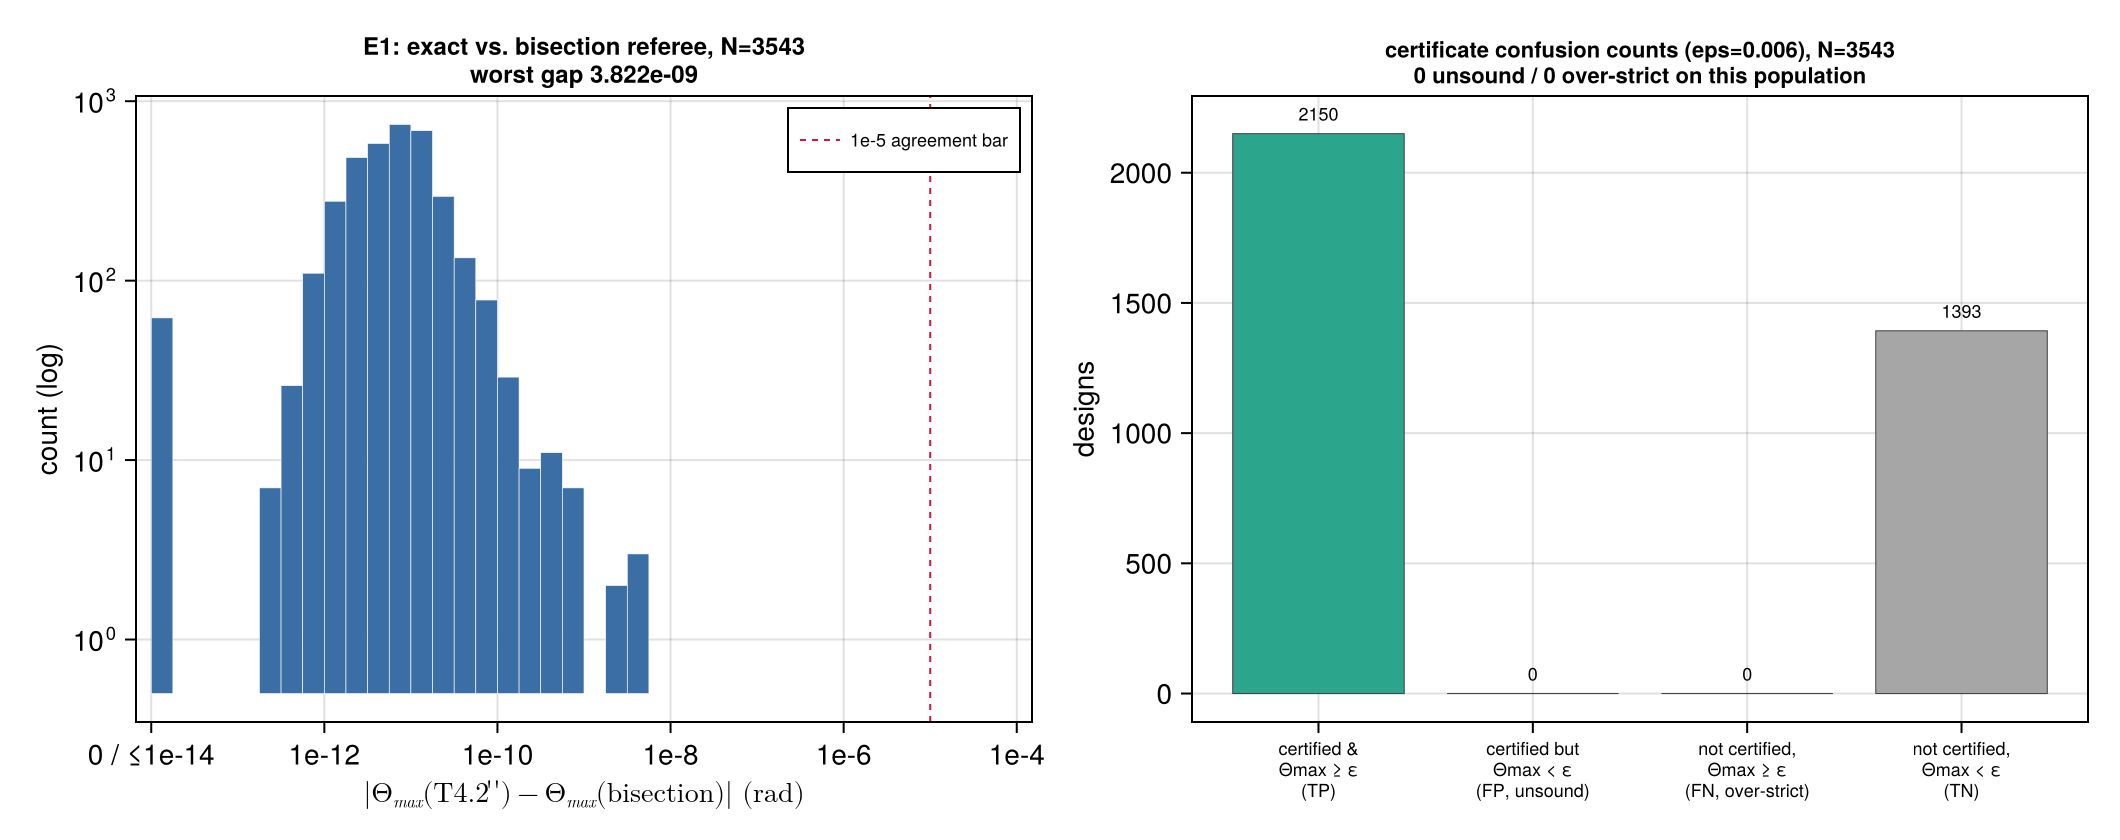
\includegraphics[width=0.84\textwidth]{../../results/final/figures/fig_e1_agreement.png}
\caption{E1 validation, $N=3{,}113$. Left: histogram (log-$y$) of
$|\Tmax(\text{closed form}) - \Tmax(\text{bisection referee})|$; every gap is at
floating-point scale. Right: the certificate's confusion counts against $\Tmax\ge\varepsilon$
at $\varepsilon=0.006$: TP $2{,}150$, FP $0$, FN $0$, TN $963$. Source
\file{results/final/e1/e1.csv}, figure \file{results/final/figures/fig\_e1\_agreement.png}.}
\label{fig:e1}
\end{figure}

\clearpage
%==============================================================================
\section{Design-space diagnostics: what fails, and why}
\label{sec:diagnostics}
%==============================================================================

With an exact range and a sound certificate in hand, we could ask a question the framework
leaves open: on a \emph{population} of planar graphs, how often is the projected embedding
$X_0$ of Eq.~\eqref{eq:eq6} actually deployable? This section reports that campaign. Every
experiment was pre-registered with a numeric bar before it was run, and the verdicts below
include several of our own hypotheses being killed.

\paragraph{The population, stated once.} 200 random graphs from
\file{kill\_common::make\_graph(id,100,800,1400)} --- Voronoi 67, Delaunay 67, quad-dominant
66 --- with $|F|\in[101,793]$, median $332.5$, each under both orientation rules, giving 400
designs. Populations are deterministic functions of the graph id, so every experiment sees
the same graphs and the numbers are directly comparable across experiments.

\paragraph{The scale caveat, also stated once.} Every reference case in the papers' own
figures has $|F|\in[4,97]$. This population is 3--8$\times$ larger by face count than
anything either paper demonstrates, and the difficulty of finding a jointly feasible
embedding scales with $|\Esplit|$, which scales with $|F|$. The generative process is
unbiased --- Voronoi/Delaunay/quad-dominant triangulations of uniform random points is a
standard way to produce ``arbitrary planar graphs'' --- but the \emph{scale} is outside what
the papers demonstrate. Both halves of that sentence are true and both are repeated wherever
the numbers appear.

\subsection{K1a: is the projection valid on random graphs?}

\textbf{[N]} 200 graphs, $10^4$ Gaussian null-space samples each plus a trust-region ladder,
wall $39.7$ s.

\begin{center}
\small
\begin{tabular}{@{}lr@{}}
\toprule
quantity & value \\
\midrule
$n_{\mathrm{inv}}(X^{\mathrm{ini}})>0$ (asserted 0) & \textbf{0} \\
$n_{\mathrm{inv}}(X_0)>0$ & 142 / 200 \\
mean inverted fraction of $X_0$ & 0.0410 (max 0.1655) \\
$p_{\mathrm{valid}}=0$ (no sample with $n_{\mathrm{inv}}=0$) & 135 / 200 \\
$X^{\mathrm{ini}}$ injective (control) & \textbf{200 / 200} \\
\textbf{$X_0$ injective (no face overlap)} & \textbf{0 / 200} \\
\textbf{some sample injective} & \textbf{0 / 200} \\
\textbf{some sample with $\Tmax>0$} & \textbf{0 / 200} \\
\bottomrule
\end{tabular}
\end{center}

\noindent Under the inverted-face measure the projection is invalid on 142/200; under the
\emph{real} criterion --- no face--face overlap in the flat state --- it is invalid on
\textbf{200/200}, and not one of the two million samples drawn is a valid embedding. 58 graphs
have every face positively oriented and \emph{still} self-intersect, which is the earlier
remark that $\POS$ certifies nothing, measured at scale.

\paragraph{What this does and does not say.} It says that on this population the usable region
is not reachable by isotropic sampling of the null space around $X_0$. It does \emph{not} say
$U(\varepsilon)$ is empty --- the authored tilings supply 187 valid deployable configurations,
which is exactly the population the validation of Section~\ref{sec:e1} runs on, and
Section~\ref{sec:rangeembed} finds deployable points in the same random-graph shape spaces by
a different route. The honest statement is that validity is a \emph{strong} constraint that
random graphs miss under this projection.

\subsection{The \texorpdfstring{$0^+$}{0+} calculus: the two exact first-order quantities}
\label{sec:zeroplus}

Every failing design is failing the same way, and the exact scan names the same culprit: at
$\theta=0^+$ two copies of a split cut translate \emph{into} each other rather than apart.
The following two quantities make that statement exact and, crucially, \emph{quadratic in the
design coordinates}, so it can be optimised rather than sampled.

\paragraph{The split-edge sign $q_e$ [A].} By Lemma~\ref{lem:t1b} the two copies of a split
edge $e=\{a,b\}$ between faces $f,g$ ($\sigma_f=\sigma_g$) are the same vector at every
$\theta$ and differ by a pure translation:
\[
y_{(v,g)}(\theta)-y_{(v,f)}(\theta) \;=\; \sin(\theta/2)\,dS_e,
\qquad dS_e := S_{(v,g)}-S_{(v,f)}
\]
(the same vector for $v=a$ and $v=b$, with $dC_e=0$ identically). So the relative motion at
$0^+$ is one fixed direction and the only question is which \emph{side} of $e$ it points to.
Take the half-edge of $e$ inside $f$ in the stored CCW order, and let
$d_e := x_{\mathrm{to}}-x_{\mathrm{from}}$; then $f$ is to the left of $d_e$ and $g$ to the
right, and the copies separate iff $g$'s copy moves right:
\begin{equation}
\boxed{\;q_e \;:=\; \det(dS_e,\,d_e)\;}
\qquad
q_e>0 \iff \text{the cut \textbf{opens}},
\qquad
q_e\le0 \iff \text{copies move into each other and }\Tmax=0 .
\label{eq:qe}
\end{equation}
Swapping the roles of $f$ and $g$ reverses \emph{both} $d_e$ and $dS_e$, and
$\det(-u,-v)=\det(u,v)$, so $q_e$ needs no per-edge sign choice.

\paragraph{The corner margin $\mu_v$ [A].} The split sign controls only split-edge copies. A
design with every $q_e>0$ and every $A_f>0$ can still have $\Tmax=0$, with the exact scan
reporting the binding contact as \emph{vertex-edge}: a corner of one face moving into the
interior of another at $0^+$. Same calculus, one step more general. At $\theta=0$ every copy
of a source vertex $v$ sits at $x_v$, so for two copies $p,a$ of $v$ (with $a$ in face $f$)
\[
y_p(\theta)-y_a(\theta) \;=\; \sin(\theta/2)\,dS, \qquad dS:=S_p-S_a
\]
\emph{exactly}, because $C_p=C_a=x_v$. With $e_1 = x_{v_{\mathrm{next}}}-x_v$ and
$e_2 = x_{v_{\mathrm{prev}}}-x_v$ the two edges of $f$ at $v$, and
\[
g_1=\det(e_1,dS), \qquad g_2=\det(dS,e_2), \qquad \mathrm{cross}=\det(e_1,e_2),
\]
the copy $p$ enters $f$ at $0^+$ iff $dS$ lies strictly inside the corner cone, which is
$\{g_1>0 \wedge g_2>0\}$ at a convex corner and its complement at a reflex one. So the
separation margin, positive exactly when $p$ stays out of $f$, is
\begin{equation}
\boxed{\;
\mu \;=\;
\begin{cases}
\max(-g_1,-g_2) & \text{convex corner } (\mathrm{cross}>0)\quad\text{--- a \textbf{disjunction},}\\
\min(-g_1,-g_2) & \text{reflex corner } (\mathrm{cross}<0)\quad\text{--- a \textbf{conjunction}.}
\end{cases}\;}
\label{eq:mu}
\end{equation}

\paragraph{Why both are exact and quadratic [A].} \file{deploy()} is linear and homogeneous
in $X$, so $dS_e(X_0+\Phi t) = dS_e(X_0)+\sum_j t_j\,dS_e(\Phi_j)$ while $d_e$, $e_1$, $e_2$
are affine in $t$. Hence $q_e$ and $\mu$ are \textbf{quadratic polynomials in $t$}, as is
every face signed area. Nothing here is sampled. The one caveat is that $\mu$ is only
piecewise smooth: the $\max/\min$ is a disjunction whose branch is chosen by
$\mathrm{cross}(t)$. Every solver in this work re-reads the branch at every evaluation and
decides feasibility by the \emph{exact} margin, never by a smoothed objective.

\paragraph{Relation to Eq.~\eqref{eq:eq9}.} With the coefficients of the next subsection,
$r=h'(0)$ is exactly Eq.~(9)'s first-order separation term, and $q_e$ is a positive multiple
of $r$. So Eq.~(9) already ``knows'' about $q_e$. What it does not do is drive $q_e$ strictly
positive on \emph{every} split edge simultaneously while keeping the flat state embedded ---
which is what the repair below asks for, and what the algorithm of
Section~\ref{sec:rangeembed} finally achieves.

\subsection{What Eq.~(9) certifies, exactly}
\label{sec:eq9}

\begin{proposition}[T5.3, the split-edge separation harmonic]
Let $e=\{a,b\}$ be a split edge between $f,g$, $d:=x_b-x_a$, $\Delta u := u_g-u_f$. The signed
separation is the orientation harmonic of $(a',b';a'')$, and by Lemma~\ref{lem:t1b}
\[
h(\theta) = \det\bigl(R_f d,\; 2sJ\Delta u\bigr)
= \sin\theta\,\det(d,J\Delta u) - \sigma_f(1-\cos\theta)\det(d,\Delta u),
\]
so in the notation of Theorem~\ref{thm:t3}
\begin{equation}
\boxed{\;p = -\sigma_f\det(d,\Delta u), \qquad q = +\sigma_f\det(d,\Delta u) = -p,
\qquad r = \det(d,J\Delta u) = \langle d,\Delta u\rangle .\;}
\label{eq:T52}
\end{equation}
Hence $p+q=0$ \emph{identically} --- the flat state is always a root, as it must be --- and
$(1+\tau^2)h(\tau) = 2\tau(r+p\tau)$. \textbf{[A]}
\end{proposition}
\noindent\textbf{[N]} On 72 split edges over 16 graphs the closed forms \eqref{eq:T52} agree
with the generic coefficients \eqref{eq:T32}, and $p+q=0$, to a worst relative deviation of
$4.37\times10^{-15}$. In the K1c run the same check reads $p+q=0$ to
\emph{exactly} $0.000\times10^{0}$ (structural) with $|{\rm closed}-{\rm generic}|/\mathrm{scale}$
at worst $8.898\times10^{-8}$, carried entirely by nearly collapsed split edges (median over
all edges $2.0\times10^{-15}$).

\begin{corollary}[the exact false-negative condition of Eq.~(9)]
Eq.~\eqref{eq:eq9} penalises the first-order separation $h'(0)=r$ and nothing else, so it
certifies $r>0$. From $(1+\tau^2)h=2\tau(r+p\tau)$ the \emph{only other} root is
$\tau^*=-r/p$, i.e.\ $\theta^*=2\arctan(-r/p)$. Given $r>0$, $\tau^*>0$ iff $p<0$. Therefore
\[
\begin{aligned}
\text{Eq.~(9) false negative at }e \iff\;\;
& r=\langle d,\Delta u\rangle>0 \;\wedge\; p=-\sigma_f\det(d,\Delta u)<0 \\
&\wedge\; \theta^*<\Tmax \;\wedge\; \text{\eqref{eq:E2} holds at }\theta^*
\;\wedge\; \text{the faces cross at }\theta^* .
\end{aligned}
\]
Eq.~(9) is blind to $p$ \textbf{by construction}: $p$ is a second-order coefficient and the
energy is a first-order test at $\theta=0$ --- the one configuration T2.3 shows to be a branch
point.
\end{corollary}

\paragraph{A drop-in replacement.} Penalise $\max(0,-p/r)$ (equivalently $\tau^*$) instead of
$\mathrm{sign}(r)$: smooth, the same $O(|\Esplit|)$ cost, and by \eqref{eq:T52} a ratio of two
quadratic forms in $X$.

\paragraph{[N] The measured rate, and a specification that was self-contradictory.} Our own
pre-registered rule for this experiment asked for the fraction of designs with a re-closure
$\theta^*<\Tmax$. \emph{That rule is unsatisfiable}, and discovering it is the finding:
the crossing clause says the interiors overlap just after $\theta^*$, while $\Tmax$ is by
definition the first angle at which any two interiors overlap, so ``$\theta^*<\Tmax$'' and
``$\theta^*$ is a genuine crossing'' are contradictory. Measured on 171 deployable embedded
designs with split cuts:

\begin{center}
\small
\begin{tabular}{@{}lrrrrr@{}}
\toprule
$Y_9$ source & certified & rule as written & clauses, same range & $\theta^*<\min\beta$ & $\theta^*$ \emph{is} binding \\
\midrule
authors' native \file{prevent}, published defaults & 169 & 110 (65.09\%) & \textbf{0} & \textbf{16 (9.47\%)} & 12 (7.10\%) \\
our \file{optimize\_collision\_sweep} ($\gamma$ ladder) & 115 & 32 (27.83\%) & \textbf{0} & 40 (34.78\%) & 9 (7.83\%) \\
\bottomrule
\end{tabular}
\end{center}

\noindent Worst $|\theta^*-\text{per-pair bisection}|$ over qualifying re-closures:
$1.035\times10^{-11}$. The $65.09\%$ headline the uncorrected experiment would have produced
is made entirely of roots that are \emph{not} collisions --- grazes, or collinearities where
the duplicates never meet as segments --- and must not be quoted; 110 of 169 of the authors'
designs would have been reported as false negatives on the strength of nothing. The two
well-posed references are $\theta^*<\min_e\beta_e$ (did Eq.~(9) leave a re-closure inside the
range the pattern would otherwise reach --- $\mathbf{9.47\%}$ on their code) and
$\theta^*=\Tmax$ (is the re-closure what actually stops deployment --- $7.10\%$).

\textbf{A side finding about our own reimplementation.} Our
\file{optimize\_collision\_sweep} collapses \textbf{109 split edges to zero length} across
this population; the authors' native \file{prevent} collapses \textbf{0}. That is why only
115 of 171 of our outputs are valid flat embeddings against 169 of 171 of theirs, and it is an
independent reason --- beyond the withdrawal recorded in Section~\ref{sec:framework} --- never
to quote our Eq.~(9) reimplementation as a baseline.

\subsection{K5: is the \emph{orientation} the problem?}

Eq.~(1) picks $\sigma$ to maximise hinge cuts and knows nothing about whether the closure
system then has a solution near $X^{\mathrm{ini}}$. K5 asks whether choosing $\sigma$ against
the \emph{deployability defect} instead fixes that.

\textbf{[D]} $D(\sigma) = \sum_{\text{holes}}\bigl\|\sum_{e\in C\cap\Ehinge}
(x_{\mathrm{dst}}-x_{\mathrm{src}})\bigr\|^2$ evaluated at $X^{\mathrm{ini}}$ --- exactly
Eq.~\eqref{eq:eq2}'s residual, so $D=0$ iff $X^{\mathrm{ini}}$ is already uniformly
deployable. $\sigma_{\mathrm{def}}$ is a greedy local search over face flips minimising $D$:
single-face and adjacent-pair flips, strictly improving moves only, any flip rejected that
makes $c(\Gamma)>1$ or detaches a face; started from $\sigma_{\mathrm{mc}}$ plus 3 random
$\sigma$, best kept, at most $20|F|$ attempts per start, deterministic seed $7000+\mathrm{id}$.

\begin{center}
\small
\begin{tabular}{@{}lrr@{}}
\toprule
quantity & $\sigma_{\mathrm{mc}}$ (Eq.~1) & $\sigma_{\mathrm{def}}$ \\
\midrule
\textbf{valid $X_0$ by the certificate, $\varepsilon=0.3$} & \textbf{0 / 200} & \textbf{0 / 200} \\
\quad of which $\POS$ alone & 58 & \textbf{186} \\
\quad $\NOOV(0.15)$ alone & \textbf{0} & \textbf{0} \\
\quad $\NOROOT(0.3)$ alone & \textbf{0} & \textbf{0} \\
\textbf{certified $\Tmax>0$} & \textbf{0 / 200} & \textbf{0 / 200} \\
median $D(\sigma)$ & $2.245\times10^{3}$ & $\mathbf{1.840\times10^{1}}$ \\
median inverted faces of $X_0$ & 9.5 & \textbf{0} \\
median $\|X_0-X^{\mathrm{ini}}\|_\infty$ / median edge & 1.587 & \textbf{0.334} \\
median $|\Esplit|$ = median $\dim\mathrm{null}$ & 126.5 & 321.5 \\
graphs with $D=0$ exactly ($X^{\mathrm{ini}}$ already deployable) & 0 & \textbf{16} \\
overlap-free $X_0$ at $\theta=0$ (the \emph{withdrawn} predicate) & 0 / 200 & 114 / 200 \\
\bottomrule
\end{tabular}
\end{center}

\paragraph{The result is the gap between two rows.} $\sigma_{\mathrm{def}}$ \textbf{fixes the
flat sheet, decisively}: the defect falls $122\times$ in the median, the projection moves the
mesh $4.7\times$ less far, median inverted faces go $9.5\to0$, $\POS$ goes $58\to186$, and on
16 graphs $X^{\mathrm{ini}}$ is \emph{already} deployable so Eq.~\eqref{eq:eq6} has nothing to
do. Eq.~(1) really is choosing a bad $\sigma$. And it \textbf{does not touch the deployment}:
$\NOOV(0.15)$ is false on all 400 designs and $\Tmax=0$ on all 400. That is not a
single-probe artefact --- a log-spaced ladder from $10^{-12}$ to $1.0$ finds an interior
overlap at the first or second rung on every graph that overlaps at all, and a direct scan
confirms overlap at $10^{-2}$, $0.1$ and $0.5$ where the shrink tolerance is not in question.

\paragraph{Why, mechanically.} $\sigma_{\mathrm{def}}$ buys its low defect by more than
\emph{doubling} the split cuts, median $126.5\to321.5$: a split edge imposes no closure
constraint, so cutting more edges fully apart makes Eq.~\eqref{eq:eq2} easy to satisfy. The
hinge graph is then sparse, the structure is barely a mechanism, and it collapses into itself
immediately. The correlation of $D$ with $|\Esplit|$ bears this out and is strongly
non-monotone across the two families: $-0.6446$ under $\sigma_{\mathrm{mc}}$, $-0.0346$ under
$\sigma_{\mathrm{def}}$.

\paragraph{The lesson.} A defect-only objective is wrong for the same reason max-cut is:
\emph{neither knows about collisions}. $\sigma$ is a real and badly-chosen design variable ---
that much is worth saying --- but no purely combinatorial objective on $\sigma$ produces a
deployable random graph. The objective has to carry a deployment term, and the certificate is
now cheap enough to be one.

\subsection{K6: is the \texorpdfstring{$0^+$}{0+} jam repairable inside the shape space?}

The null space is large (median $\dim\mathrm{null}$ 126 under $\sigma_{\mathrm{mc}}$, 321
under $\sigma_{\mathrm{def}}$), so: is there a point in it at which every cut opens outward?
The repair minimises, over $t$,
\begin{equation}
F(t) = \sum_{\Esplit}\mathrm{softplus}(-q_e/s) + \sum_{F}\mathrm{softplus}(-A_f/s)
\;\bigl[+\,w_c\sum\mathrm{softplus}(-\mu/s)\bigr]
\;+\; w_p\frac{\|X(t)-X_0\|^2}{Ns} \;+\; \lambda\|t\|^2 ,
\label{eq:k6obj}
\end{equation}
$s=(\text{median edge})^2$, by our L-BFGS from $t=0$ and 3 Gaussian starts of scale
$0.1\,\mathrm{med}$, $\max\_\mathrm{iter}=1200$, seed $6000+7\,\mathrm{id}$. Two variants on
the same designs and seeds: \emph{primary} = split + vertex-edge with proximity
($w_c=0.05$, $w_p=10^3$), \emph{secondary} = split-only ($w_c=w_p=0$). Feasibility is always
decided by the exact constraint values.

\begin{center}
\footnotesize
\begin{tabular}{@{}lrr@{}}
\toprule
quantity & $\sigma_{\mathrm{mc}}$ & $\sigma_{\mathrm{def}}$ \\
\midrule
\textbf{inward split edges at $t=0$} (q1 / median / q3 / max) & 32 / \textbf{65.5} / 122 / 265 & 58 / \textbf{103.5} / 194 / 340 \\
median inward \emph{fraction} of split edges & \textbf{0.500} & \textbf{0.342} \\
designs with \textbf{zero} inward split edges at $t=0$ & \textbf{0 / 200} & \textbf{0 / 200} \\
inward corner incidences at $t=0$ (q1 / median / q3 / max) & 121 / \textbf{215.5} / 412 / 670 & 150 / \textbf{252.5} / 469 / 798 \\
median $\min q$ at $t=0$ & $-77.81$ & $-130.43$ \\
$0^+$-feasible, primary variant & 0 / 200 & 2 / 200 \\
$0^+$-feasible, secondary (split-only) & \textbf{60 / 200} & \textbf{67 / 200} \\
\textbf{certified $\Tmax>0$, all four variants} & \textbf{0 / 200} & \textbf{0 / 200} \\
binding contact at the primary failures & split-inward 200 & split-inward 188, vertex-edge 11, inverted 1 \\
\bottomrule
\end{tabular}
\end{center}

\paragraph{Verdict: FAIL, 0\% against a 20\% bar, on both $\sigma$ and all four variants.}
And the failure is informative. The repair problem is \emph{solvable} on a quarter of the
designs --- $\min q>0$ and $\min\mu>0$ on 127 of 400 under the split-only objective --- and
solving it buys \textbf{zero} deployment range, because a fresh contact is waiting behind the
one that was repaired. Fixing $q$ moves the binding event from \texttt{split-inward} to
\texttt{vertex-edge} and then to \texttt{inverted}. \emph{The obstruction is not one bad sign
but the whole first-order cone being empty.}

\paragraph{The \file{first\_root} bug, recorded in full.} An intermediate pass reported exact
$\Tmax>0$ on 15/200 $\sigma_{\mathrm{mc}}$ designs, all Delaunay, which looked like a partial
rescue. It was not. \file{validity\_certificate} set \file{cert.first\_root} to the
\emph{first} admissible deflated root the (face-pair, vertex, edge) loop happened to meet,
not the \emph{smallest} over all candidates; callers use it as the supremum of $\varepsilon$
for which $\NOROOT(\varepsilon)$ holds, so any candidate scanned after the true first contact
could inflate the reported range. The independent bisection caught it: on those same 15
designs it gives $\Tmax>0$ on only 13, and the three disagreements are \file{delaunay\_7}
(exact $2.4658$, bisection $0$), \file{delaunay\_82} ($2.1144$ vs $0$) and
\file{delaunay\_127} ($3.0229$ vs $5.96\times10^{-4}$). The fix is the three-line guard now at
\file{Kirigami/src/method/contact.jl:339} --- keep a root only if it is smaller than the
incumbent. The corrected pass gives $\Tmax>0$ on \textbf{0/400}, and a confirmatory rerun
reproduces every aggregate exactly. \emph{The certified count was 0 both before and after};
the bug never introduced a certificate, only an inflated exact $\Tmax$.

\paragraph{And a bug on the other side, F34.} The refereeing bisection is \emph{not} ground
truth either. On \file{voronoi\_93} it reported a collision of faces $(94,184)$ from
$\theta=10^{-7}$ that a $1200\times1200$ grid and 17{,}280 radial probes show does not exist.
Cause: \file{polygons\_overlap} shrank each copy of the shared pin \emph{differently}, so
pin-incident edge pairs acquired orientation determinants of size $10^{-11}\dots10^{-17}$
whose signs decided a strict crossing test --- flipping with the shrink and with $\theta$, and
failing when a sector is reflex. The predicate was rewritten: no shrinking, edges split at all
intersections, piece midpoints classified by a 3-state point-in-polygon, and a long-double
orientation predicate with tolerance relative to edge length and scale, clamped to
$[10^{-14},10^{-9}]$. The referee is now tolerance-independent, agreeing at $10^{-12}$,
$10^{-9}$ and $10^{-6}$ alike. \textbf{The bias was one-sided (downward), so no verdict
moved}; what changed is that K6 reads $2/400$ exact (still uncertified) rather than $0/400$,
K5's $\sigma_{\mathrm{def}}$ embedding rate reads $125/200$ rather than $114/200$, and K9's 36
positives referee $36/36$ rather than $32/36$. \file{derivation\_tests} R6-c1 pins the
resolution: $0$ common interior points of $1{,}442{,}401$ probes.

\subsection{T-1: the mechanism is reflex corners created by the projection}
\label{sec:t1exp}

The theorist persona proposed a per-vertex balance theorem: Eq.~\eqref{eq:eq2} at a
\emph{pure} vertex (one touched by no split edge) should force the $0^+$ separation velocities
to positively span the plane, so no copy can enter a neighbour. Split cuts break the balance.
The kill test: over K6's 400 designs, count interior vertices touched by no split edge whose
$0^+$ margin is non-positive. PASS $=0$.

\textbf{[N]} \file{results/kill/t1/t1\_summary.txt}, 7 s off the K6 cache:

\begin{center}
\small
\begin{tabular}{@{}lr@{}}
\toprule
quantity & value \\
\midrule
interior vertices with $\ge2$ copies & 165{,}788 \\
\quad pure (no incident split edge) & 14{,}886, on 250/400 designs \\
\quad touched ($\ge1$ incident split edge) & 150{,}902 \\
\textbf{balance holds exactly at pure vertices} & $\max|\delta_v| = 1.999\times10^{-14}$ \\
$N_{\mathrm{bad}}$ (pure, $\mu_v\le0$) & \textbf{1{,}968}, on 142/400 designs \\
\quad binding incidence at a \textbf{convex} corner & \textbf{2} \\
\quad binding incidence at a \textbf{reflex} corner & \textbf{1{,}966} \\
pure vertices with \emph{every} incidence at a convex corner & 12{,}919, of which bad \textbf{1} \\
\textbf{faces non-convex at $X_0$} & \textbf{22{,}103 / 156{,}220} \\
\textbf{faces non-convex at the input embedding} & \textbf{0} \\
collapse rate: pure vs touched & $0.1322$ vs $0.4408$ \\
$\mathrm{corr}(|\delta_v|,\mu_v)$ on touched & Spearman $+0.0616$, Pearson $-0.1016$ \\
\bottomrule
\end{tabular}
\end{center}

\paragraph{Verdict: FAIL --- and the residue is the most useful thing in the diagnostic half.}
Balance \emph{does} hold, exactly, at every pure vertex, and the designs collapse anyway.
Balance is not the predictor; the correlation with the margin is essentially zero. What
\emph{is} the predictor is convexity: $1{,}966$ of the $1{,}968$ failures are at a
\textbf{reflex} corner, and a pure vertex all of whose incidences are convex fails on
\textbf{1 of 12{,}919}.

\paragraph{And the reflex corners are introduced by the projection.} The input embeddings
--- Voronoi cells, Delaunay triangles, convex random quads --- have \textbf{zero} non-convex
face corners. The Eq.~\eqref{eq:eq6} projection produces \textbf{22{,}103 of 156{,}220}. Read
against \eqref{eq:mu} this is exactly the right mechanism: at a convex corner the margin is a
\emph{disjunction}, satisfied as soon as the relative velocity leaves either half-plane; at a
reflex corner it is a \emph{conjunction} and needs both. The unconstrained least-norm
projection has no term that prevents this, so it walks the mesh into the one corner geometry
where the $0^+$ condition is hardest to satisfy.

\emph{A correction to our own record.} An earlier log entry claimed T-1 was contradicted by
K6 ``because Eq.~(2) holds''. That reason was wrong: balance does hold per vertex. The
conclusion fails for a different reason, and the different reason is what the constructive
half of the work is built on.

\subsection{B4: is it the fixed boundary that empties the space?}

Two readings of the emptiness result cannot be told apart by K6 alone: K6 measures $0/400$ on
fixed-boundary patches, while the same Voronoi generator on \emph{tori}
(Section~\ref{sec:periodic}) gives $11/12$ $0^+$-feasible and $4/12$ certified. The
populations differ in exactly one thing --- the patch carries Eq.~\eqref{eq:eq4}'s fixed
boundary rows $B$, the torus does not. B4 tests three variants on K6's population verbatim:
\texttt{fixed} ($[L;B]X=[0;T]$, the control), \texttt{free} ($B$ dropped entirely, replaced by
pinning one vertex --- the only gauge $L$ cannot see is the global translation, since every
$L$ row sums to zero; rotation and scaling are left in because $q_e$ is rotation-invariant and
positively homogeneous), and \texttt{split\_free} ($B$ restricted to boundary vertices
touching no split edge). PASS bar: exact $\Tmax>0$ on $\ge10\%$ of the 400 \texttt{free}
designs.

\noindent\textbf{[N] Provenance (Julia port, 2026-09-20).} The \texttt{free} rows that reach
$\Tmax>0$ (\file{voronoi\_93}: $0.2484$~rad, \file{voronoi\_96}: $0.241884$~rad) and their
feasibility flags are knife-edge outcomes of a non-converged 1\,199-iteration L-BFGS run: with
bit-identical $X_0$, $\Phi$ the C++ and Julia iterates agree to $10^{-15}$ for about 20 iterations and
then diverge by rounding (\file{derivations/scratch/b4\_path/README.md}). They are archived values,
not reproducible numbers.

\begin{center}
\small
\begin{tabular}{@{}llrrrrr@{}}
\toprule
variant & $\sigma$ & median $\dim\mathrm{null}$ & median $\min q$ at $t{=}0$ & $0^+$-feasible (split-only) & \textbf{exact $\Tmax>0$} & certified \\
\midrule
\texttt{fixed} & mc & 126 & $-78.20$ & 60 & \textbf{0} & 0 \\
\texttt{split\_free} & mc & 131 & $-66.98$ & 83 & \textbf{0} & 0 \\
\texttt{free} & mc & 156 & $-51.55$ & \textbf{176} & \textbf{0} & 0 \\
\texttt{fixed} & def & 321 & $-130.64$ & 67 & \textbf{0} & 0 \\
\texttt{split\_free} & def & 329 & $-130.64$ & 182 & \textbf{0} & 0 \\
\texttt{free} & def & 338 & $-130.64$ & \textbf{200} & \textbf{2} & 2 \\
\bottomrule
\end{tabular}
\end{center}

\paragraph{Verdict: FAIL --- $2/400 = 0.50\%$ against a 10\% bar, and $1/400$ refereed.}
Three things the run nevertheless establishes.

\begin{enumerate}\itemsep3pt
\item \textbf{The dimension count is exactly right.}
$\dim\mathrm{null}(\texttt{free})-\dim\mathrm{null}(\texttt{fixed}) = |V_\partial|-1$ on
\textbf{400/400} rows (mean gain $32.8$; the $-1$ is the pin). The mechanism B4 proposes is
present and measurable; it is its \emph{consequence} that fails.
\item \textbf{The boundary really does constrain the $0^+$ cone, and that buys almost no
range.} The split-only relaxation goes $60/200\to176/200$ under $\sigma_{\mathrm{mc}}$ and
$67/200\to\mathbf{200/200}$ under $\sigma_{\mathrm{def}}$ when $B$ is dropped, monotonically
through \texttt{split\_free}. None of it survives contact with the corner margin: the binding
contact simply migrates, \texttt{split-inward} $\to184$, \texttt{vertex-edge} $\to13$,
\texttt{inverted} $\to1$ --- the same migration K6 reported. \emph{The first-order cone is not
emptied by the boundary rows; it is emptied by the number of simultaneous sign conditions},
and $|V_\partial|\approx33$ extra dimensions against 126--321 split-sign constraints does not
change that.
\item \textbf{One genuine positive, and one that does not survive the referee.}
\file{voronoi\_96} ($\sigma_{\mathrm{def}}$, \texttt{free}, $|F|=497$, 866 split edges,
$\dim\mathrm{null}=947$, $\min q = 0.1418$) has exact $\Tmax = \varepsilon_{\max} =
\text{bisection} = 0.24188$ --- agreed by all three independent labels, and the first random
planar graph in the project with a positive refereed deployment range. \file{voronoi\_93}
reads $0.24840$ by the scan and certificate and $0$ by the bisection; that disagreement was
the F34 referee artefact, and the scan was later confirmed right. Both positives sit
$10.3$ and $12.9$ median edge lengths from $X_0$: where the free boundary helps at all, it
helps by leaving the neighbourhood of the projection entirely.
\end{enumerate}

\noindent \textbf{Consequence for the headline.} ``The published boundary condition empties
the space'' is \textbf{not licensed}. The space is essentially empty either way, and the
torus advantage of Section~\ref{sec:periodic} is \emph{not} explained by the absence of $B$.

\subsection{K8a: is there a non-uniform flex that escapes?}

Everything so far tests the \emph{uniform} branch. K8a asks the structural question: does
\emph{any} first-order flex --- uniform or not --- separate every cut and every corner
simultaneously?

\noindent\textbf{[N] Provenance (Julia port, 2026-09-20).} Every combinatorial and geometric column of
K8a reproduces exactly. The archived LP-layer values (margins, dual bounds, the ``dual-certified''
tallies) predate the C++ solver fix \texttt{d38b0a4} and are superseded by the rerun; the
$\sigma$-chart on non-deployable $X^{\mathrm{ini}}$ and the margins on the truncated-square family
depend on a degenerate-row artefact in \file{normalise\_rows} and are not reproducible in either
implementation (\file{results/kill/k8a\_julia/PROVENANCE.md}).

\paragraph{The rows [A].} A flex assigns every face $(\omega_f,w_f)$ with
$V_f(y)=\omega_fJy+w_f$, and the pins impose $V_f(p_i)=V_g(p_i)$, which is exactly the
rigidity matrix. Because at $\theta=0$ every copy of a source vertex sits at $x_v$ and $X$ is
held fixed, every $0^+$ separation condition of Section~\ref{sec:zeroplus} becomes a
\textbf{strict linear inequality in the flex}:
\begin{align}
\text{split edge } e:\quad & \mathrm{row}_e = \det\bigl(V_{f_1}(x_v)-V_{f_0}(x_v),\; d_e\bigr) \;=\; q_e/2, \label{eq:rowsplit}\\
\text{corner incidence:}\quad & \mathrm{row}_{G_1} = -g_1 = \det(dV,e_1), \qquad
\mathrm{row}_{G_2} = -g_2 = -\det(dV,e_2), \qquad \mu = \mu_{0^+}/2 . \label{eq:rowcorner}
\end{align}
\textbf{[N]} Both identities are asserted \emph{exactly} (to $10^{-9}$ relative) against
\file{zero\_plus\_q} and \file{zero\_plus\_corner\_margin} at the $\sigma$ ray, in a unit test,
on three tilings. The flex basis is $\ker A$ (dense SVD) plus the integrated translations plus
one free translation pair per component of $\Gamma$; a unit test checks
$\dim\ker R = \dim\ker A + 2c(\Gamma)$ against an independent dense QR rank, checks
orthonormality, and checks the uniform ray lies in the span. Over all 277 configurations,
$\max\|RN\|/\max|R| = 7.8\times10^{-14}$.

\paragraph{The branch charts, and the honest asymmetry.} At a reflex corner the margin is a
$\min$, so both rows are required and the constraint is convex. At a convex corner it is a
$\max$, so the feasible set is a \emph{union} of two half-spaces and $P(X)$ is a union of
$2^{n_{\mathrm{convex}}}$ polyhedra. Every one of the $244{,}931$ corner incidences on this
population at $X^{\mathrm{ini}}$ is at a convex corner, so no enumeration is possible. Four
passes are run: pass 0 is the conjunctive relaxation (a \emph{subset} of $P(X)$, needing no
branch choice); pass 1 is the branch the uniform ray itself selects; passes 2--3 repair the
branch from the best witness so far. Fixed points were reached at pass 2 or 3 on every graph.
\textbf{Feasibility of any pass proves $P(X)\ne\varnothing$. Infeasibility of the passes tried
proves nothing} --- what supports the negative reading is the dual bound, not the failure to
find a witness.

\paragraph{The LP, and the two-sided bracket.} With rows normalised to unit norm, the quantity
solved for is the matrix-game value
\begin{equation}
\mathrm{val} \;=\; \max_{\|z\|_2\le1}\ \min_i\ a_i\!\cdot\! z
\;=\; \min_{\lambda\in\Delta}\ \bigl\|A^{\!\top}\lambda\bigr\|_2 .
\label{eq:conelp}
\end{equation}
Both sides are $\ge0$ (take $z=0$), and $\mathrm{val}>0$ iff the strict system is feasible.
\emph{Every iterate of either loop is feasible for its side}, so the reported margin is a
rigorous lower bound and the dual bound a rigorous upper bound: the solver never has to be
trusted, and a small dual bound is an approximate Farkas certificate. The solver is local
code, no LP library.

\paragraph{[N] The result.}
\begin{center}
\small
\begin{tabular}{@{}lrr@{}}
\toprule
 & at $X^{\mathrm{ini}}$ & at $X_0$ \\
\midrule
\textbf{LP margin $>0$} & \textbf{0 / 100} & \textbf{0 / 100} \\
$\mathrm{dual}_{\max}<10^{-6}$ (every chart tried certified) & 84 / 100 & 68 / 100 \\
$\mathrm{dual}_{\max}$ median & $9.9\times10^{-8}$ & $1.0\times10^{-7}$ \\
$\sigma$ is a flex of the framework & 0 / 100 & 100 / 100 \\
$\sigma\in P(X)$ & 0 / 100 & 0 / 100 \\
$\dim\ker A$, median & 17 & 65 \\
rows, median & \multicolumn{2}{c}{4{,}911 (142 split, 2{,}338 corner incidences)} \\
\bottomrule
\end{tabular}
\end{center}

\noindent \textbf{Verdict: FAIL, $0/100$ against a bar of $\ge20/100$ --- and the failure is
structural.} On 84 of 100 graphs there is a non-negative combination of the split-edge and
corner rows summing to within $10^{-6}$ of zero: an approximate Farkas certificate that
\emph{no flex at all}, uniform or not, separates every cut and every corner at first order.
The soundness control passes 4/4: on the four split-bearing authored tilings $\sigma$ is
reported inside $P(X)$ and the LP independently finds a strictly positive margin
($5.40\times10^{-1}$, $7.35\times10^{-1}$, $3.53\times10^{-2}$, $3.12\times10^{-1}$); on the
extended control of 73 configurations, $\sigma\in P(X)$ on 71 and margin $>0$ on 72.
Euler-step sanity: on every configuration with a positive margin the witness flex is
integrated one explicit Euler step and tested for overlap --- \textbf{72 of 72 collision-free},
64 of them already at half a median edge of vertex travel.

\paragraph{The one genuine rescue.} \file{snub\_square\_R20\_s1}, a shape-space sample of the
snub-square tiling, has $\sigma$ \emph{outside} $P(X)$ ($\min q_e=-6.05\times10^{-2}$, so the
uniform deployment collides at $0^+$ and $\Tmax=0$) and the LP nevertheless certifies a
strictly positive \emph{non-uniform} margin of $4.31\times10^{-2}$, with a collision-free
Euler step at the largest tested amplitude. The mechanism is real and does fire; it simply
never fires on any of the 100 random graphs.

\paragraph{F38: the solver was wrong and the certificates were not.} This is worth recording
in full because it is the sharpest self-catch in the project. \file{cone\_lp} computed the two
ends of its bracket with two unrelated algorithms. The dual end (Frank--Wolfe on
$\min_\lambda\|A^{\!\top}\lambda\|$) was sound. The primal end came from a \emph{separate}
log-sum-exp smoothing loop --- about 1{,}000 projected-gradient steps of size
$\mu/\sigma_{\max}^2\approx10^{-5}$, started at $z=0$, in a space of dimension up to 300
against 5{,}000 rows --- and was the \emph{only} source of the returned witness. But the
Frank--Wolfe iterate $w=A^{\!\top}\lambda$ \emph{is} the optimum: at the minimum-norm point of
$\mathrm{conv}\{a_i\}$ one has $a_i\!\cdot\!w\ge\|w\|^2$ for every $i$, so $z=w/\|w\|$ attains
$\min_i a_i\!\cdot\!z\ge\|w\|$ and the bracket closes. The fix is away-step Frank--Wolfe on
the min-norm point with the primal witness read off the same iterate, plus
\file{sigma\_chart\_margin} (the uniform ray on its own chart, computed with no solver in the
loop --- a rigorous lower bound the solver must beat) and \file{farkas\_residual}, which
recomputes $\|A^{\!\top}\lambda\|$ row by row and checks $\lambda\ge0$, $\sum\lambda=1$.

\begin{center}
\small
\begin{tabular}{@{}lrr@{}}
\toprule
on K9's 30 embeddings, regenerated bit-identically & old solver & corrected \\
\midrule
$\sigma\in P(X)$ by direct \file{zero\_plus} measurement & 23 & 23 \\
\quad \dots LP margin $>0$ & \textbf{0 / 23} & \textbf{23 / 23} \\
\quad \dots margin $\ge$ the solver-free $\sigma$-chart bound & --- & 23 / 23 \\
$\sigma$ \emph{outside} $P(X)$, margin $>0$ anyway & 0 / 7 & \textbf{6 / 7} \\
feasible overall & \textbf{0 / 30} & \textbf{29 / 30} \\
\bottomrule
\end{tabular}
\end{center}

\noindent Margin / $\sigma$-chart bound: median $\mathbf{8.73}$, range $2.06$--$56.9$. So the
earlier ``expansive-cone LP: 30 run, 0 feasible'' line is a \textbf{solver artefact and must
not be quoted}. The dual certificates, by contrast, were real: over all 277 configurations
the worst $\min_i\lambda_i$ is exactly $0$ and the worst $|\sum\lambda-1|$ is
$2.5\times10^{-13}$; independently verified at $10^5$ dual steps, $\|A^{\!\top}\lambda\|<10^{-6}$
on \textbf{96/100} ($X^{\mathrm{ini}}$) and \textbf{99/100} ($X_0$), and $<10^{-9}$ on
$65/100$ and $57/100$. Per family at $X^{\mathrm{ini}}$, verified $<10^{-9}$: Voronoi
$34/34$, quad-random $31/33$, Delaunay $0/33$ (29/33 at $10^{-6}$) --- the Delaunay residue is
Frank--Wolfe convergence, not a different phenomenon. \textbf{The $0/100$ margin count and the
FAIL verdict are unchanged.}

\paragraph{Caveats, stated.} (i) Infeasibility is \emph{certified to $10^{-6}$}, not proved:
the dual bound is a numerical Farkas residual, not an exact rational certificate, and it is
per branch chart. (ii) The branch enumeration is not exhaustive and cannot be --- $2^{2338}$
charts per graph, of which four are visited. A positive result would have been a proof; the
negative result is evidence. (iii) The $\dim\ker A$ medians here (Voronoi 3, quad-random 17,
Delaunay 72) are \emph{not} the mobility figure of 305 quoted elsewhere: that is $\dim\ker A$
on the 2-core of a different population at a different size distribution. The two must not be
quoted side by side. (iv) The margin is scale-dependent through the row normalisation; only
its \emph{sign} is invariant.

\subsection{A3: the jitter ladder, and how the certificate bug was found}

The sharpest objection to the emptiness result is that it compares 0/200 random graphs against
8/8 authored tilings, and a reader cannot separate ``the design space is empty'' from ``our
generator and our orientation heuristic fail on our random graphs'', because random patches
differ from authored tilings in every respect at once. The separating experiment is an
interpolation with the \emph{combinatorics held fixed}: jitter an authored tiling's interior
vertex positions continuously and watch deployability die.

\textbf{[N]} The 8 authored reference tilings, with
$X[v]\leftarrow X[v]+a\cdot(\text{median edge})\cdot\mathcal{N}(0,I)$ on interior vertices
only, $a$ on \textbf{20 log-spaced steps in $[0.005,1.0]$}, \textbf{20 seeds} each, plus an
$a=0$ baseline: 3{,}208 designs $\times$ 2 $\sigma$ rules $=$ 6{,}416 rows, 12 shards, wall
$2.2$ s. Boundary vertices are not jittered because the pipeline solves with a fixed boundary.

\paragraph{Finding 1: half the authored population is outside the problem.} Four of the eight
reference cases --- \file{rotating\_squares}, \file{triangles\_alternating},
\file{kagome\_3636}, \file{periodic\_squares\_4x4} --- are \textbf{split-free} under their own
$\sigma$. For these $\dim\mathrm{null}=0$, so the fixed-boundary system has a \emph{unique}
solution, and the authored positions already satisfy it. The Eq.~\eqref{eq:eq6} projection
therefore sends \emph{any} jittered interior geometry back to the authored tiling exactly:
measured $\|X_0-X_{\mathrm{base}}\|_\infty = 0.0000$ at every amplitude up to $a=1.0$, while
$\|X_0-X^{\mathrm{ini}}\|_\infty$ reaches $2.8$ median edges. Those four curves are flat at
$1.0$ not because they tolerate jitter but because \textbf{they never left the start point}.
A unit test pins this. \emph{Any claim of the form ``authored tilings pass 8/8'' is really
``4 trivially, 4 substantively''}, and that qualifier is now attached everywhere.

\paragraph{Finding 2: on the four split-bearing tilings the transition is real and sharp.}

\begin{center}
\small
\begin{tabular}{@{}lrrrr@{}}
\toprule
tiling ($\sigma_{\mathrm{mc}}$) & $a^*$ ($\Tmax>0$) & $a$ at frac $\ge0.9$ & $a$ at frac $\le0.1$ & width \\
\midrule
\file{snub\_square\_33434} & 0.163 & 0.107 & 0.248 & 0.36 dec \\
\file{hexagons\_auto} & 0.277 & 0.142 & 0.573 & 0.61 dec \\
\file{truncated\_square\_488} & 0.320 & 0.248 & 0.573 & 0.36 dec \\
\file{tiling\_3\_4\_3\_12} & 0.522 & 0.248 & 0.757 & 0.48 dec \\
\bottomrule
\end{tabular}
\end{center}

\noindent Deployability survives perturbations of order \emph{one sixth} of an edge length and
dies around one third to one half. Under $\sigma_{\mathrm{def}}$ the thresholds are uniformly
smaller ($0.071$ / $0.188$ / $0.096$ / already dead at $0.005$), consistent with K5 and K6:
the defect-minimising orientation buys nothing here and doubles to quintuples $|\Esplit|$.
Over all split-bearing rows, $\Tmax>0$ on $1225/1604$ ($76.4\%$) under $\sigma_{\mathrm{mc}}$
and $634/1604$ ($39.5\%$) under $\sigma_{\mathrm{def}}$.

\paragraph{Finding 3, which decided the verdict and found F32.} At the \emph{smallest}
amplitude $a=0.005$, every split-bearing tiling has $\POS$ 20/20, $\NOOV$ 20/20 and exact
$\Tmax$ between $1.0$ and $2.4$ rad on 20/20 seeds --- and the certificate passes on
$0/20$, $0/20$, $5/20$, $10/20$. \textbf{$\NOROOT$ is the only clause that fails.} An
infinitesimal perturbation of an exactly symmetric tiling splits a degenerate contact and
pushes a \emph{graze} root into $(0,0.006)$ while the first real overlap stays at $\approx2$
rad. Over the split-bearing ladder, \textbf{1{,}622 of the 1{,}859 rows with $\Tmax>0$ are not
certified: an 87.3\% false-negative rate.} That measurement is what triggered the diagnosis
and the F32 fix of Section~\ref{sec:certificate}; after the fix the same rows re-measure at
\textbf{0.0\%}, and $a^*(\text{certified}) = a^*(\Tmax>0)$ on every tiling. The ``the
certificate is knife-edge'' reading is \textbf{withdrawn} --- it was a bug, not a property of
the geometry.

\paragraph{Predictors: the bar is met only by a restatement of the mechanism.}

\begin{center}
\footnotesize
\begin{tabular}{@{}lrrr@{}}
\toprule
predictor & AUC($\Tmax>0$), all rows & AUC, split-bearing & AUC(certified), split-bearing \\
\midrule
$\rho_{\mathrm{geom}}$ (the proposed ratio) & 0.918 & \textbf{0.778} & 0.532 \\
$\rho_{\mathrm{hop}}$ & 0.892 & 0.706 & 0.611 \\
$\rho_{\max}$ & 0.952 & 0.870 & 0.580 \\
$p_{\mathrm{split}}=|\Esplit|/|F|$ & 0.874 & 0.657 & 0.713 \\
\textbf{badq\_ini} (fraction of split edges with $q_e\le0$ at $X^{\mathrm{ini}}$) & 0.987 & \textbf{0.976} & 0.704 \\
aniso & 0.745 & 0.816 & 0.590 \\
$D(\sigma)$ & 0.585 & 0.504 & 0.628 \\
amp (positive control) & 0.743 & 0.831 & 0.577 \\
margin\_$X_0$ ($X_0$ control) & 1.000 & 1.000 & 0.621 \\
badq\_$X_0$ ($X_0$ control) & 1.000 & 1.000 & 0.727 \\
\bottomrule
\end{tabular}
\end{center}

\noindent The AUC routine was cross-checked against an independent brute-force
Mann--Whitney count on \file{badq\_ini} ($0.012789$ vs $0.0128$). The bar was AUC $\ge0.9$;
only \file{badq\_ini} clears it, and ``some split cut already opens the wrong way at
$X^{\mathrm{ini}}$'' \emph{is} the K5/K6 failure mode, not an independent geometric
characteristic. The proposed ratio $\rho$ reaches only $0.778$.

\paragraph{Verdict: MIXED, FAIL as literally written.} It \emph{does} answer the objection in
part: emptiness is a function of measured geometry, reached continuously from patterns whose
combinatorics were never randomised, with a transition amplitude that is neither 0 nor 1. It
\emph{does not} deliver a generator-independent predictor.

\begin{figure}[t]
\centering
\includegraphics[width=0.84\textwidth]{../../results/kill/jitter/transition.png}
\caption{The jitter ladder. Deployable fraction, certified fraction and median $\Tmax$ against
jitter amplitude $a$ in median edge lengths, per tiling, both $\sigma$ rules. Grey curves are
the four \emph{split-free} tilings, whose Eq.~(6) projection undoes any interior jitter
exactly, so they carry no signal. On the four split-bearing tilings the transition is monotone
and $0.36$--$0.61$ decades wide, with $a^*\in[0.16,0.52]$ under $\sigma_{\mathrm{mc}}$.
Source \file{results/kill/jitter/\{jitter.csv, ladder.csv\}}.}
\label{fig:jitter}
\end{figure}

\clearpage
%==============================================================================
\section{The range-maximising constrained embedding}
\label{sec:rangeembed}
%==============================================================================

This is the constructive deliverable. It keeps the framework's cut rules, its hole
preimages, its linear system \eqref{eq:eq4} and its shape space \eqref{eq:eq5} exactly as
published, and changes only \emph{which point of the shape space is selected}. The
development went through three experiments --- K9, K9b, K9c --- and the two failures are as
informative as the success, so all three are reported.

\subsection{K9: the convexity and split-outward barriers}

\paragraph{The hypothesis, straight out of T-1.} Section~\ref{sec:t1exp} measured that the
reflex corners which jam the mechanism are \emph{created} by the unconstrained projection,
not by the graph. So put them back inside the shape space. Inside $X(t)=X_0+\Phi t$:
\begin{equation}
\min_t\ \|X(t)-X^{\mathrm{ini}}\|_F^2
\quad\text{s.t.}\quad
\mathrm{cross}_i(t)\ \ge\ \delta \;\;\text{for every corner }i\text{ of every face},
\quad\bigl[\,q_e(t)\ \ge\ \delta'\;\text{for every split cut}\,\bigr],
\label{eq:k9}
\end{equation}
with $\mathrm{cross} = \det(x_v-x_{v_{\mathrm{prev}}},\,x_{v_{\mathrm{next}}}-x_v)$, positive
exactly at a strictly convex corner of a CCW face.

\begin{remark}[the convexity constraint subsumes the area constraint]
Every corner strictly convex implies every face convex \emph{and} positively oriented, so
\eqref{eq:k9} subsumes the face-area constraint of the K6 repair \eqref{eq:k6obj}. Note also
that $\mathrm{cross}$ is the \emph{same} quantity whose sign selects the branch in
\eqref{eq:mu}: with $e_1=x_{v_{\mathrm{next}}}-x_v$, $e_2=x_{v_{\mathrm{prev}}}-x_v$ we have
$\det(e_1,e_2)=\mathrm{cross}$. So inside the convexity barrier the reflex branch of $\mu$
cannot occur.
\end{remark}

\begin{remark}[the objective is $\|t\|^2$ in disguise]
$X_0$ is the orthogonal projection of $X^{\mathrm{ini}}$ onto the affine solution set, so
$X^{\mathrm{ini}}-X_0\perp\mathrm{range}(\Phi)$ and, with $\Phi$ orthonormal from the SVD,
$\|X(t)-X^{\mathrm{ini}}\|_F^2 = \|X_0-X^{\mathrm{ini}}\|_F^2 + \|t\|^2$. The code
nevertheless evaluates the true distance so that nothing depends on $\Phi$ being exactly
orthonormal.
\end{remark}

\paragraph{How it is solved, and the honesty rule.} Both constraint families are quadratic in
$t$ and the feasible set is \emph{not convex}, so this is a heuristic and is reported as one.
Phase A (feasibility) minimises $\sum_i\mathrm{softplus}((\tau-\mathrm{cross}_i)/s)$ plus the
split terms plus $\lambda\|t\|^2$, with a continuation over the target
$\tau\in\{0.01,0.1,1\}\times\delta$, warm-started, from $t=0$ and Gaussian restarts. Phase B
(proximity) minimises the distance behind a log barrier $B(u)=-\log u$ linearly extended below
$u_0$ (so the backtracking line search never sees an infinity), with the weight decreased
geometrically, keeping \emph{only strictly feasible} iterates.

\begin{quote}
\textbf{The rule that governs every solver in this report.} \textsc{feasible} always means the
\emph{exact} constraint values at the returned point, never the value of a penalty or a
barrier. An infeasible or zero-range answer is a statement about \emph{this solver}, never a
proof that the constrained slice is empty. The headers say so, so that no caller can report
it otherwise.
\end{quote}

\paragraph{[N] Result: the first non-zero on random graphs, and a FAIL.} Settings
$\delta=\delta'=10^{-3}\mathrm{med}^2$, 3 Gaussian starts of scale $0.1\,\mathrm{med}$ plus
$t=0$, 600 L-BFGS iterations per stage, 6 barrier stages, $\varepsilon=0.3$; three arms per
design on K6's exact 400 designs.

\begin{center}
\footnotesize
\begin{tabular}{@{}lrrr@{}}
\toprule
quantity & $X_0$ (control) & (a) convexity only & (b) convexity $+$ split \\
\midrule
convex-feasible designs & 79 / 400 & \textbf{115 / 400} & 30 / 400 \\
\textbf{exact $\Tmax>0$} & \textbf{0} & \textbf{0} & \textbf{36 / 400 (9.0\%)} \\
refereed (fixed predicate) & 0 & 0 & \textbf{36} \\
certified ($\varepsilon_{\max}>0$) & 0 & 0 & \textbf{36} \\
all $0^+$ corner margins $\mu>0$ at the returned $X$ & 0 / 79 & 0 / 115 & \textbf{23 / 30} \\
median $\min\mu/\mathrm{med}^2$ over feasible & $-8.79$ & $-9.89$ & $\mathbf{+4.96\times10^{-2}}$ \\
$\|X-X^{\mathrm{ini}}\|$ per vertex, median (median edges) & 0 & 0.271 & 0.376 \\
binding contact at $\Tmax=0$ & split-inward 400 & split-inward 400 & split-inward 260, inverted 72, vertex-edge 32 \\
\bottomrule
\end{tabular}
\end{center}

\noindent Verdict: \textbf{FAIL}, $9.0\%$ against a pre-registered $10\%$ bar --- missed by 4
designs --- while every comparable baseline on the same 400 designs is exactly zero.
$\varepsilon_{\max}$ median $0.253$, max $1.997$ rad, with $33$ of $36$ at
$\ge0.1$ rad; per orientation $\sigma_{\mathrm{mc}}$ $24/200$ and $\sigma_{\mathrm{def}}$
$12/200$.

\paragraph{Two lessons that survive the FAIL.}
\begin{enumerate}\itemsep2pt
\item \textbf{Convexity alone is necessary, not sufficient.} Arm (a) raises convex feasibility
from 79 to 115 designs and buys \emph{exactly zero} deployment range --- the binding contact
stays \texttt{split-inward} on all 400. The two constraints together are what moves the count
off zero, which is the same lesson K6 reached from the other side (split-only feasible on
126/400, certified 0). Non-convex corners at $X_0$: $35{,}323/656{,}736 = 5.38\%$.
\item \textbf{Feasibility is not necessary for deployment.} Only $23$ of the $36$ positives
are feasible at the full margin $\delta'$; the other 13 miss the margin the solver was aiming
at and deploy anyway. So \file{kiri\_design} reports \texttt{feasible} and $\Tmax$ as separate
facts and ranks designs by $\Tmax$, never by feasibility (judgement call 13).
\end{enumerate}

\subsection{K9b: more search makes it worse, and that is the diagnosis}

K9b holds the population, the shape space and the certificate fixed and pushes only the
solver: 8 Gaussian starts $+\,t=0$ plus two warm starts, 10 barrier stages (K9: 6), a sweep of
$\delta=\delta'$ over $\{10^{-4},10^{-3},3\!\cdot\!10^{-3},10^{-2}\}\mathrm{med}^2$, and a
stage 2 running the softmin-of-first-contact objective gated on exact improvement.

\begin{center}
\small
\begin{tabular}{@{}lrrr@{}}
\toprule
quantity & K9 (b) & \textbf{K9b sweep} & best over both \\
\midrule
exact $\Tmax>0$ & 36 / 400 (9.0\%) & \textbf{28 / 400 (7.0\%)} & 37 / 400 (9.25\%) \\
certified, of which $\varepsilon_{\max}\ge0.1$ rad & 36, 33 & 28, 16 & 37, 34 \\
$\varepsilon_{\max}$ median / max (rad) & 0.253 / 1.997 & 0.147 / 1.828 & 0.253 / 1.997 \\
graphs with $\ge1$ deployable $\sigma$ (of 200) & 33 & 26 & 34 \\
\bottomrule
\end{tabular}
\end{center}

\noindent Roughly $4\times$ the search budget moved the count \emph{down}. Referee agreement
is exact: worst $|\text{exact}-\text{bisection}|$ $2.8\times10^{-7}$ over all 400, soundness
$400/400$. Of the levers, only the $\delta$ sweep paid: among K9b's 28 positives the winning
margin is $10^{-2}\mathrm{med}^2$ on 15, $10^{-3}$ on 12, $10^{-4}$ on 1 --- the constraint
should be posed with a \emph{generous} margin. Stage 2 supplied the accepted point on 2 of 28,
and it was gated on $\Tmax>0$, so it never ran on the feasible-but-jammed designs where it
would have mattered: a design error in that driver, stated as such.

\paragraph{The nine lost designs are the whole point.} K9b keeps 27 of K9's 36 positives, adds
1, and \textbf{loses 9}. All nine are Delaunay, and on all nine K9b's returned point is
\emph{exactly feasible} --- every corner cross and every split sign clears the margin --- and
still has $\Tmax=0$, binding \texttt{vertex-edge}. Two solvers found \emph{different points
inside the same feasible set}, one deployable and one not.

\begin{quote}
\textbf{Margin feasibility does not determine deployability.} What caps the yield near 9\% is
therefore not the search budget and not the feasible set, but \textbf{the objective that
selects the point inside it} --- and that objective is proximity, $\|X-X^{\mathrm{ini}}\|$,
which knows nothing about deployment.
\end{quote}

\subsection{K9c: the range as the objective}

K9c keeps the population, the shape space, the barriers and the certificate fixed and replaces
\emph{only} the objective.

\subsubsection{Stage A: maximise the exact \texorpdfstring{$0^+$}{0+} margin}

\paragraph{The scalar.} In units of $s=\mathrm{med}^2$,
\begin{equation}
\boxed{\;m(X) \;=\; \frac{1}{s}\,\min\Bigl(\min_{e\in\Esplit} q_e(X),\;\;\min_j \mu_j(X)\Bigr)\;}
\label{eq:margin}
\end{equation}
--- the joint minimum of the two first-order separation families of
Section~\ref{sec:zeroplus}. The design deploys at $0^+$ exactly when both families are
strictly positive.

\paragraph{Flattening, and the branch modes.} $m$ is a minimum of quantities quadratic in $t$,
except that $\mu$ carries the $\max/\min$ disjunction. The margin list is flattened into plain
smooth entries $c_i(t)$:
\begin{itemize}\itemsep1pt
\item one entry $q_e$ per split edge;
\item at a \emph{convex} corner, \textbf{one} entry $-g_j$ with $j=\arg\max(-g_1,-g_2)$ read at
the current point --- a lower bound on $\mu=\max(-g_1,-g_2)$, and \emph{equal} to it at the
point where the mode was read;
\item at a \emph{reflex} corner, \textbf{two} entries $-g_1$ and $-g_2$, whose min is exactly
$\mu$ there.
\end{itemize}

\paragraph{The surrogate, and the lemma that makes it safe.}
\begin{lemma}[softmin lower bound]
\label{lem:softmin}
For $\kappa>0$,
\[
M_\kappa(t) \;=\; -\kappa\,\log\sum_i \exp\!\bigl(-c_i(t)/(s\kappa)\bigr)
\;\;\le\;\; \min_i c_i(t)/s ,
\]
with equality in the limit $\kappa\to0$. Combined with the mode choice above,
$M_\kappa(t)\le m(X(t))$ for \emph{every} $t$ and every choice of modes.
\end{lemma}
\noindent So maximising $M_\kappa$ maximises a \emph{certified lower bound} on the $0^+$
margin, and the reported $m$ is always the exact minimum over the exact margins, never the
surrogate. Two unit tests check exactly those two claims
(\file{Kirigami/test/test\_range\_embed.jl}), and two more finite-difference the analytic
gradient of the whole stage-A objective --- softmin plus both log barriers, split term and
corner term --- against a central difference on two tilings and two barrier weights.

\paragraph{The analytic gradient.} With softmin weights
$w_i = \exp(-c_i/(s\kappa))/\sum_{i'}\exp(-c_{i'}/(s\kappa))$,
\[
\frac{\partial M_\kappa}{\partial t} \;=\; \frac{1}{s}\sum_i w_i \frac{\partial c_i}{\partial t},
\qquad
\frac{\partial}{\partial t}\Bigl[w\!\sum_i B\bigl((\mathrm{cross}_i-\delta)/s\bigr)\Bigr]
= \frac{w}{s}\sum_i B'\!\bigl((\mathrm{cross}_i-\delta)/s\bigr)\frac{\partial\,\mathrm{cross}_i}{\partial t},
\]
and each $c_i$, $\mathrm{cross}_i$, $q_e$ is quadratic in $t$, so every
$\partial c_i/\partial t$ is an explicit \emph{affine} function of $t$ --- one matrix--vector
product each, no finite differences and no adjoint solve.

\subsubsection{Stage B: push the exact \texorpdfstring{$\Tmax$}{Theta max} in a trust region}

From a point with $m>0$, stage B maximises the exact range with the softmin-of-first-contact
objective of \file{range\_opt.jl}, whose gradients are the implicit-function-theorem
derivatives of the root map:
\begin{equation}
\frac{\partial\theta_\pi}{\partial t_i}
\;=\; -\,\frac{\partial_{t_i}p + \cos\theta_\pi\,\partial_{t_i}q + \sin\theta_\pi\,\partial_{t_i}r}
{-q\sin\theta_\pi + r\cos\theta_\pi} ,
\label{eq:T62}
\end{equation}
the denominator being $h'_\pi(\theta_\pi)$, non-zero exactly when the root is simple. Because
$p,q,r$ are quadratic in $t$, the numerator's derivatives are affine in $t$.
\textbf{[N]} Verified against central differences to a relative error of
$3.9\times10^{-7}$.

Stage B runs under a \textbf{shrinking trust region} --- caps of $0.25$, $0.10$, $0.04$ median
edges on $\|X-X_{\mathrm{prev}}\|_\infty$ --- and accepts a step only when \emph{all four} of
these exact conditions hold: exact convexity, exact split signs, a margin floor
$m\ge\tfrac12 m_0$, and an actual improvement in the exact $\Tmax$.

\begin{quote}
\textbf{Stated as a weakness, not hidden.} The margin constraint in stage B is enforced by
exact rejection plus the trust region, \emph{not} by a barrier inside \file{range\_opt}'s
objective. That is weaker than a barrier, and it is why the trust region is needed at all.
\end{quote}

\paragraph{And a caveat on the gradients.} $\theta_\pi(t)$ is \emph{not} differentiable where
the root is double ($\mathrm{disc}=0$) or where the active pair changes; the softmin smooths
the second, not the first. A double root is exactly where a contact appears or disappears ---
precisely where a range-maximising optimiser wants to sit. That the non-smooth set is
negligible along the optimiser's path is a \textsc{conjecture}, not proved; a
subgradient/bundle fallback is the honest remedy if line searches start failing. The active
set is likewise a heuristic with \emph{no} size guarantee (H-LOC is refuted,
Section~\ref{sec:contact}); its \emph{soundness} comes from the exact refresh, and it must
never be called a certified active set.

\subsubsection{Full pseudocode}

\begin{algorithm}[t]
\caption{\texttt{design\_range\_max} --- the deliverable (K9c). \file{method/range\_embed.jl}, \file{method/design.jl}}
\label{alg:k9c}
\begin{algorithmic}[1]
\Require mesh $M$, orientation $\sigma$, input embedding $X^{\mathrm{ini}}$, options, seed
\Ensure the best design found, its exact characterisation, and its \emph{provenance}
\State build the cut structure; $[L;B]\gets$ \Call{AssembleSystem}{$M,\sigma$}; $(X_0,\Phi)\gets$ dense SVD solve \Comment{Eqs.~\eqref{eq:eq4}--\eqref{eq:eq6}}
\State $\mathrm{med}\gets$ median edge length; $s\gets\mathrm{med}^2$
\Statex \textbf{-- proximity arms (controls, and warm starts) --}
\State $t_{k9}\gets$ \Call{ConvexEmbed}{$\delta=\delta'=10^{-3}s$, 3 starts $+\,t{=}0$, 6 barrier stages, 600 iters, seed}
\State $t_{k9b}\gets$ \Call{ConvexEmbed}{$\delta=\delta'=10^{-2}s$, 8 starts, 10 stages, warm start $t_{k9}$, seed$+101$}
\Statex \textbf{-- stage A: maximise the exact $0^+$ margin, from three starts --}
\ForAll{$t_{\mathrm{start}} \in \{\,t_{k9},\ t_{k9b},\ 0\,\}$}
  \State $t\gets t_{\mathrm{start}}$; $w\gets w_0=10^{-2}$
  \For{stage $=1..S$} \Comment{$S=6$ continuation stages}
    \State modes $\gets$ \Call{RangeEmbedModes}{$X(t)$} \Comment{argmax branch per convex corner; both rows if reflex}
    \State $t\gets$ \Call{LBFGS}{$F_w$, $t$, $I$ iters} where
      $F_w(t) = -M_\kappa(t) + w\bigl[\sum_i B(\tfrac{\mathrm{cross}_i-\delta}{s}) + \sum_e B(\tfrac{q_e-\delta'}{s})\bigr]$
      \Comment{$I=120$}
    \If{$X(t)$ is \emph{exactly} feasible} keep $t$ if its \emph{exact} $m$ beats the incumbent \EndIf
    \State $w\gets 0.5\,w$
  \EndFor
  \Statex \textbf{-- stage B: convert margin into angular range --}
  \If{$m(X(t))>0$}
    \State $m_0\gets m(X(t))$; $\Theta\gets$ \Call{ExactThetaMax}{$X(t)$}
    \ForAll{caps $\in\{0.25,0.10,0.04\}\cdot\mathrm{med}$}
      \For{round $=1..8$}
        \State $t'\gets$ \Call{RangeOptStep}{$t$, softmin of first-contact roots, gradients \eqref{eq:T62}, 10 iters, $\|X(t')-X(t)\|_\infty\le$ cap}
        \State accept $t\gets t'$ \textbf{iff} exact convexity \textbf{and} exact split signs \textbf{and} $m(X(t'))\ge\tfrac12 m_0$ \textbf{and} $\Tmax(X(t'))>\Theta$
      \EndFor
    \EndFor
  \EndIf
  \State record the candidate with its provenance tag (\texttt{k9c/x0}, \texttt{k9c/x0+B}, \texttt{k9c/k9+B}, \dots)
\EndFor
\State \Return the candidate with the largest \emph{exact} $\Tmax$ (ties broken by $\varepsilon_{\max}$), together with \Call{Characterize}{$\cdot$}: exact $\Tmax$, the contact list, and $\POS\wedge\NOOV(\varepsilon/2)\wedge\NOROOT(\varepsilon)$ with the largest certifiable $\varepsilon$
\end{algorithmic}
\end{algorithm}

\paragraph{Defaults, exactly as the run used them.} $\delta=\delta'=10^{-3}\mathrm{med}^2$,
$\delta_{\mathrm{wide}}=10^{-2}\mathrm{med}^2$, softmin temperature
$\kappa=5\times10^{-3}$ (in $\mathrm{med}^2$), \textbf{6 continuation stages $\times$ 120
L-BFGS iterations} for stage A, 600 iterations for the two proximity arms, stage B on,
$\varepsilon=0.3$ rad, barrier weight $w_0=10^{-2}$ halved per stage. The three arms are
seeded $\mathrm{seed}$, $\mathrm{seed}+101$, $\mathrm{seed}+211$, with
$\mathrm{seed} = 9300+7\,\mathrm{id}+\mathrm{which}$.

\begin{quote}
\textbf{The stage settings are part of the reproduction recipe, not a tuning detail.} The
library's own defaults are $8\times200$; the run used $6\times120$. On
\file{delaunay\_130} $\sigma_{\mathrm{mc}}$ the $t=0$ start reaches $m=0.278991$ and the K9
start $0.277041$ --- a $0.7\%$ difference --- and the first opens fully under stage B
($\Tmax=\pi$) while the second reaches $2.6899$. A replay using library defaults instead of
the run's settings therefore lands on a different design. That is exactly what happened in an
earlier reproduction attempt, and the diagnosis of ``floating-point non-determinism'' it
produced was \textbf{wrong}.
\end{quote}

\subsubsection{Determinism (U10)}

\file{design\_range\_max}, \file{design\_constrained}, \file{design\_baseline} and
\file{characterize} are \textbf{pure functions} of $(\text{mesh},\sigma,X^{\mathrm{ini}},
\text{options},\text{seed})$. Nothing in \file{src/} reads the clock, spawns a thread,
iterates an unordered container or touches global state, and BLAS is pinned to one thread
(\file{BLAS.set\_num\_threads(1)}) so every reduction runs in one fixed order. Repeated calls are
bit-identical and \file{test/test\_design.jl} checks that. Two consequences worth stating:

\begin{enumerate}\itemsep2pt
\item The null-space basis $\Phi$ is the trailing block of $V$ from a dense SVD. It is
determined only up to an orthogonal transformation \emph{inside} the null space, and L-BFGS in
$t$-space is \emph{not} invariant under one. A design is reproducible against a different
Julia/BLAS version or assembly order only if $\Phi$ is \textbf{carried along, not recomputed}.
(Verified: cached and freshly recomputed bases agree bit-for-bit on this toolchain.)
\item \file{apps/kill\_k9c.jl} is the one place that was genuinely non-deterministic: it
skips stage-A starts once a per-design \emph{wall-clock} budget is exceeded, so its answer
depends on machine load. \file{--deterministic} disables that gate; \file{design\_range\_max}
never had it.
\end{enumerate}

\noindent \textbf{[N] Bulk replay, not just locked rows.} Replaying the first 134
$\sigma_{\mathrm{mc}}$ rows of \file{k9c.csv} through \file{design\_range\_max} reproduced the
archived \file{best\_src} provenance on \textbf{134 of 134} and the archived
\file{theta\_exact} on \textbf{134 of 134} to the CSV's six printed digits.
\file{test/test\_design.jl} locks four rows to $10^{-9}$: \file{delaunay\_130}
$\sigma_{\mathrm{mc}}$ (\texttt{k9c/x0+B}, $\Tmax=\varepsilon_{\max}=\pi$, i.e.\ the hero),
\file{delaunay\_148} $\sigma_{\mathrm{mc}}$ (\texttt{k9}, $1.996778$ --- the proximity arm
wins outright), \file{voronoi\_30} (\texttt{k9c/x0}, $0.0118065$, infeasible-but-deploying)
and \file{voronoi\_42} (\texttt{k9}, $0.239961$).

\subsubsection{Complexity and timings}

Per stage-A iteration the cost is $O(|\Esplit| + |\text{corner incidences}|)$ evaluations of
quadratics, each a matrix--vector product against a $2k$-dimensional $t$. Stage B additionally
enumerates candidate roots over the surviving face pairs, which is $O(n^2)$ in the worst case
and empirically $12.69$ pairs per face after the broad phase. The certificate and the exact
scan are the same enumeration. The dominant one-off cost is the dense SVD of the
$(H+B)\times N$ system, $O(N^3)$ --- worst measured solve $3.4$ s at $\approx3$k faces.

\textbf{[N] Timings.} One full \file{kiri\_design} solve on the hero graph
($|F|=101$, $\dim\mathrm{null}=16$): $0.5$ s for all six arms including the certificate.
K9c over 400 designs ran as 12 disjoint shards on a machine shared with eleven other
concurrent experiments (load average 110--145). E1's exact scan plus referee plus certificate
costs $352.1$ s summed over 3{,}113 designs, i.e.\ about $0.11$ s per design.

\subsection{Results}

\begin{center}
\footnotesize
\begin{tabular}{@{}lrrrr@{}}
\toprule
quantity & \texttt{k9} (prox.) & \texttt{k9b} (prox., $\delta{=}10^{-2}$) & \textbf{\texttt{k9c} (range-max)} & best of 3 \\
\midrule
convexity $+$ split feasible & 30 (7.5\%) & 24 (6.0\%) & \textbf{256 (64.0\%)} & 211 \\
\quad of which $0^+$ margin $m>0$ & 23 & 12 & \textbf{244} & 209 \\
\textbf{exact $\Tmax>0$} & 36 (9.0\%) & 27 (6.8\%) & \textbf{307 (76.8\%)} & \textbf{307} \\
refereed at shrink $10^{-12}$ / $10^{-9}$ & --- & --- & --- & \textbf{307 / 307} \\
certified ($\varepsilon_{\max}>0$) & 36 & 27 & \textbf{306} & 306 \\
\quad of which $\varepsilon_{\max}\ge0.1$ rad & 33 & 14 & \textbf{207} & \textbf{214} \\
$\varepsilon_{\max}$ median / q90 / max (rad) & 0.253 / 0.540 / 2.00 & 0.115 / 0.470 / 1.83 & \textbf{0.254 / 1.23 / 3.14} & 0.278 / 1.23 / $\pi$ \\
$0^+$ margin $m$ over feasible, median ($\mathrm{med}^2$) & 0.050 & 0.004 & \textbf{0.440} & 0.419 \\
\bottomrule
\end{tabular}
\end{center}

\paragraph{The baseline column, and why the jump is the objective.} On this exact population
every baseline is \textbf{0/400}: Eq.~\eqref{eq:eq6} alone (K1a), $\sigma_{\mathrm{mc}}$ and
$\sigma_{\mathrm{def}}$ (K5), all four K6 repairs, convexity alone (K9 arm a), the
boundary-relaxed system (B4), the expansive-cone LP (K8a), and the authors' own pipeline
(Section~\ref{sec:baselines}). Crucially, the two \emph{proximity} arms measured here on the
same 400 designs land at $9.0\%$ and $6.8\%$, reproducing K9's published $9.0\%$ and K9b's
$7.0\%$. That is the control which says the jump is the \textbf{objective}, and not a change
of population, solver infrastructure or referee.

\begin{center}
\small
\begin{tabular}{@{}lrrrrrr@{}}
\toprule
arm & $N$ & deployable ($\Tmax>0$) & certified & $\varepsilon_{\max}\ge0.1$ rad & median $\varepsilon_{\max}$ & max $\varepsilon_{\max}$ \\
\midrule
Eq.~(6) $+$ repairs (K6) & 400 & 0 & 0 & 0 & --- & --- \\
K9 proximity & 400 & 36 & 36 & 33 & 0.253 & 1.997 \\
K9b & 400 & 27 & 27 & 14 & 0.115 & 1.828 \\
\textbf{K9c range-max} & 400 & \textbf{307} & \textbf{306} & 207 & 0.254 & \textbf{3.142} \\
best-of-3 per design & 400 & 307 & 306 & 214 & 0.278 & 3.142 \\
\bottomrule
\end{tabular}
\end{center}

\paragraph{Per orientation and per family.} $\sigma_{\mathrm{mc}}$ $155/200$ ($77.5\%$) with
86 at $\varepsilon_{\max}\ge0.1$ rad; $\sigma_{\mathrm{def}}$ $152/200$ ($76.0\%$) with
\textbf{128} --- the orientation asymmetry K9 and K9b measured has essentially closed, but
$\sigma_{\mathrm{def}}$'s positives open wider. Per family: Voronoi $\mathbf{122/134}$,
Delaunay $\mathbf{108/134}$, quad-random $\mathbf{77/132}$. Taking the better $\sigma$ per
graph, \textbf{185 of the 200 graphs} carry a deployable design and \textbf{152} carry one
with $\varepsilon_{\max}\ge0.1$ rad.

\paragraph{Provenance of the winning point (400 designs).} Arm \texttt{k9} wins on 106
(most of these are designs where all three arms return $\Tmax=0$ and the tie-break keeps the
first arm), arm \texttt{k9b} on 2, a K9c point on \textbf{292}
(\texttt{k9c/x0} 135, \texttt{k9c/x0+B} 143, \texttt{k9c/k9+B} 7, \texttt{k9c/k9b+B} 7).
Within K9c the $t=0$ start supplies the winner on \textbf{278} and the two warm starts on 14:
\emph{the range objective does not need K9's feasible point to start from}, and reaches better
points from the raw Eq.~\eqref{eq:eq6} projection. Stage B supplies the winning point on
\textbf{157 of the 307 positives}; stage A alone gets 244 of 400 designs into the $m>0$ region
against 23 for the proximity arm. \textbf{Neither stage is sufficient alone.}

\paragraph{The price.} $\|X-X^{\mathrm{ini}}\|$ per vertex is median \textbf{0.734} median
edges, against K9's $0.38$ and K9b's $0.21$. Range is bought with distance from the input
embedding; that is what the objective is trading.

\paragraph{Yield is not scale-free, and the trend is plotted rather than averaged away.}
Binning the population by $|F|$ with Wilson 95\% intervals, Delaunay falls from about $1.0$ to
$0.8$ across the bins and quad-random from $0.75$ to $0.43$ (Figure~\ref{fig:yield}). The
method is not scale-free and that must be reported with the headline count. Why the yield
falls --- split-cut density, aspect ratio, or the solver's basin --- is \textbf{unknown}, and
it is the first question a careful reader will ask.

\paragraph{Feasibility $\ne$ deployability, revisited.} In the completed 400-design merge there
are \textbf{no margin-feasible-but-jammed designs left}: every design that reaches the
convexity and split-inward margin under the range objective also deploys
(Figure~\ref{fig:feasdep}). The nine exactly-feasible, $\Tmax=0$ designs that motivated K9c
were a property of the \emph{proximity} arms, not of the constrained set --- and all nine are
recovered by the K9c arm alone, $9/9$, which is the direct test of K9b's diagnosis. The
constraint pair remains a necessary filter and is \emph{not} claimed as the mechanism.

\paragraph{What still binds on the 93 designs that fail.} \texttt{split-inward} on
\textbf{57}, \texttt{inverted} on \textbf{27}, \texttt{vertex-edge} on \textbf{9}. The
\texttt{inverted} count is new --- K9 and K9b never returned an inverted face because their
barrier point was always feasible. Here, when no start reaches feasibility, the driver records
the \emph{least-infeasible} point honestly (\file{best\_feas}$=0$) rather than discarding it.

\paragraph{A referee disagreement, which runs the other way.} On \file{delaunay\_34}
$\sigma_{\mathrm{def}}$ the exact scan reports $\Tmax=0.387$ and the bisection reports
$1.058$. The bisection walks a grid of $\pi/4000\approx7.9\times10^{-4}$ rad and can step over
a collision interval narrower than that; the exact scan cannot, because it tests the overlap
status \emph{at the closed-form contact angles themselves}. The exact scan is therefore the
smaller and the conservative number here, the certificate is below both, and nothing in the
count depends on which is preferred.

\begin{figure}[t]
\centering
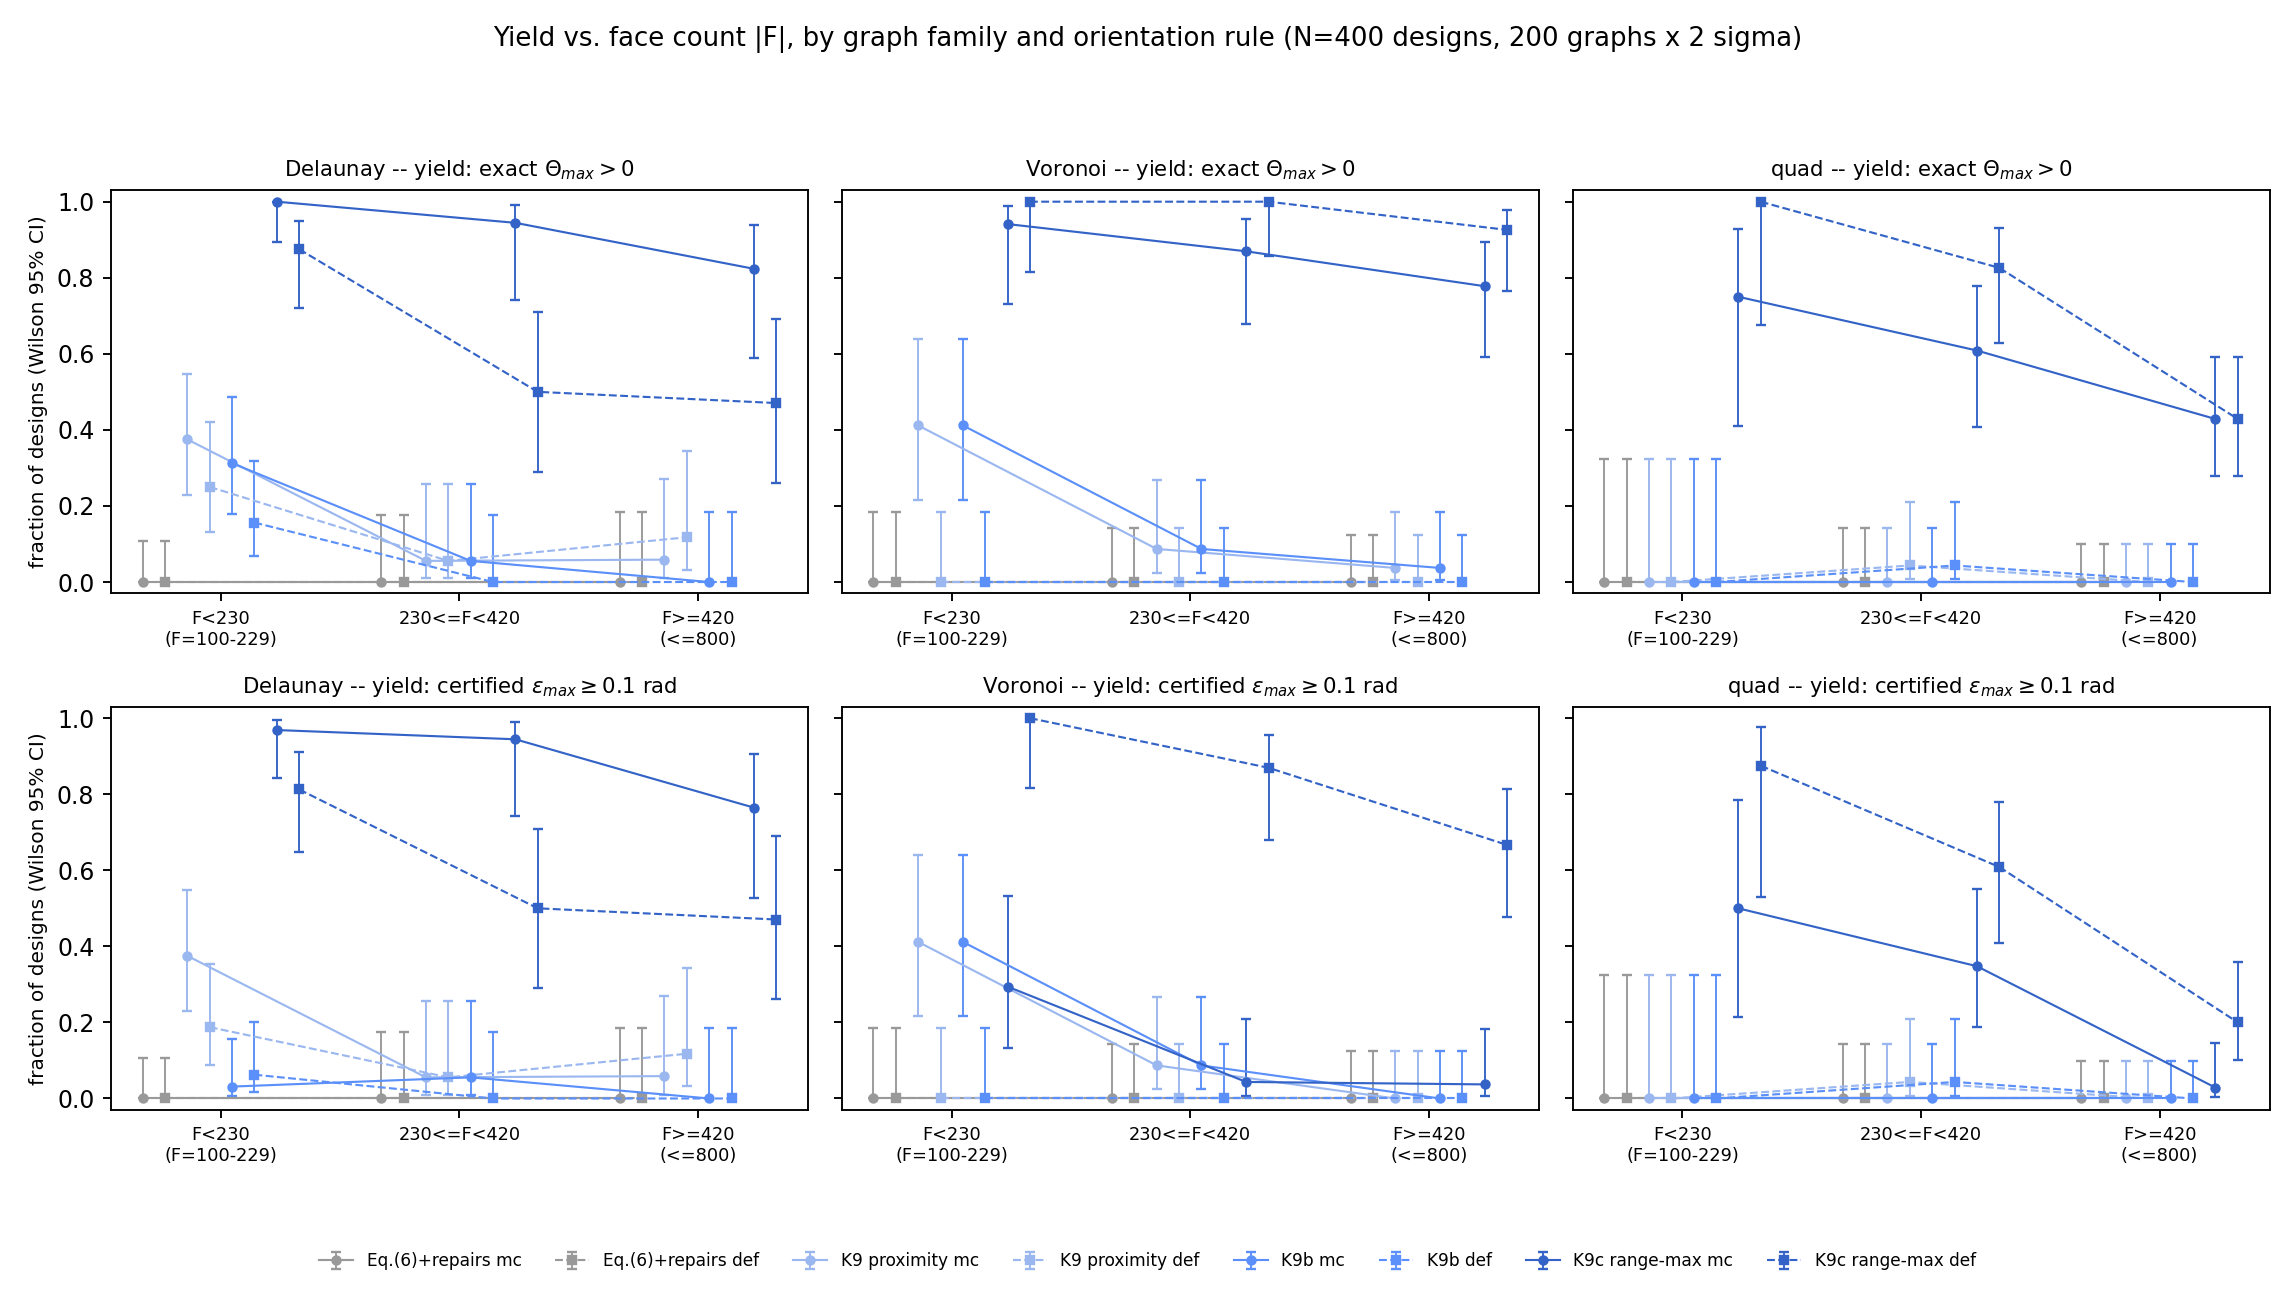
\includegraphics[width=0.86\textwidth]{../../results/final/figures/fig_yield.png}
\caption{Yield against face count $|F|$ in three bins, per family (Delaunay / Voronoi /
quad-random) and per $\sigma$ rule, for four arms (baseline Eq.~(6)$+$repairs, K9 proximity,
K9b, K9c range-maximising), with Wilson 95\% intervals. Top row: exact $\Tmax>0$. Bottom row:
certified $\varepsilon_{\max}\ge0.1$ rad. The baseline is identically zero everywhere.
Source \file{results/kill/k9c/shard\_*.csv} merged, $N=400$; baseline confirmed
independently from \file{results/kill/k6/k6\_final.csv}.}
\label{fig:yield}
\end{figure}

\begin{figure}[t]
\centering
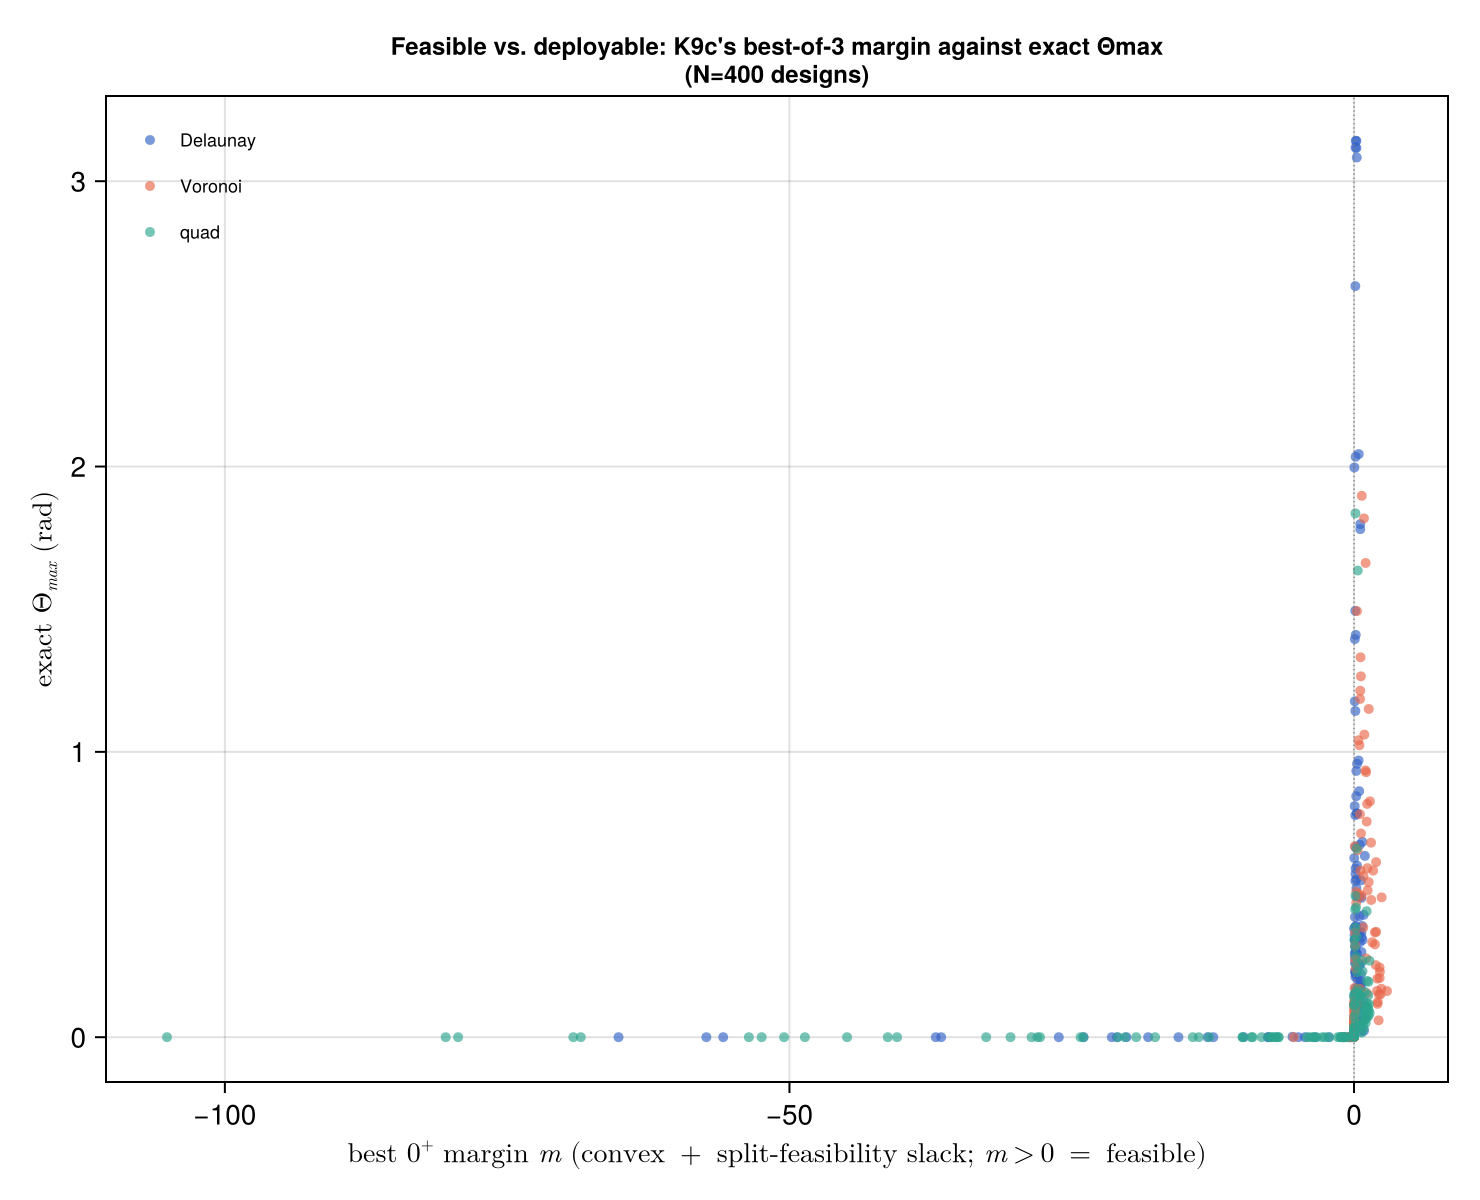
\includegraphics[width=0.66\textwidth]{../../results/final/figures/fig_feasible_vs_deployable.png}
\caption{Best $0^+$ margin (convexity $+$ split feasibility slack) against exact $\Tmax$ for
every one of the 400 designs, coloured by family, with margin-feasible-but-$\Tmax=0$ designs
ringed. Under the range objective no such design remains; the nine that motivated K9c were a
property of the proximity arms.}
\label{fig:feasdep}
\end{figure}

\begin{figure}[t]
\centering
\includegraphics[width=0.80\textwidth]{../../results/kill/k9c/k9c_gallery.png}
\caption{Gallery of K9c designs, each shown closed and at $\Tmax/2$, sorted by certified
$\varepsilon_{\max}$ ($|F|$ from 101 to 378, $\varepsilon_{\max}$ from $0.68$ to $\pi$). The
full, non-curated gallery of \emph{every} deployable design is
\file{results/final/figures/fig\_gallery\_full.png}; it is rendered deliberately without
selection. Slivers --- short edges and sharp angles --- are visible and are an acknowledged
geometric-quality caveat, the same one the 2026 paper's Limitation~1 names.}
\label{fig:gallery}
\end{figure}

\begin{figure}[t]
\centering
\includegraphics[width=0.32\textwidth]{../../export/hero2/hero2_130_sigma_mc_closed.png}\hfill
\includegraphics[width=0.32\textwidth]{../../export/hero2/hero2_130_sigma_mc_open_half.png}\hfill
\includegraphics[width=0.32\textwidth]{../../export/hero2/hero2_130_sigma_mc_open_0.9tm.png}
\caption{The hero design (\file{delaunay} id 130, $\sigma_{\mathrm{mc}}$), rendered from the
laser-cut SVG at $\theta=0$, $\Tmax/2$ and $0.9\,\Tmax$. Exact
$\Tmax=\varepsilon_{\max}=\pi$: it opens fully. Reproduced in $0.5$ s by
\file{kiri\_design export/hero2/hero2\_input.json --sigma json --seed 10210}, where
$10210=9300+7\cdot130$; the returned embedding agrees with the archived
\file{hero2\_graph.json} to $7\times10^{-15}$ per coordinate.}
\label{fig:hero}
\end{figure}

\begin{figure}[t]
\centering
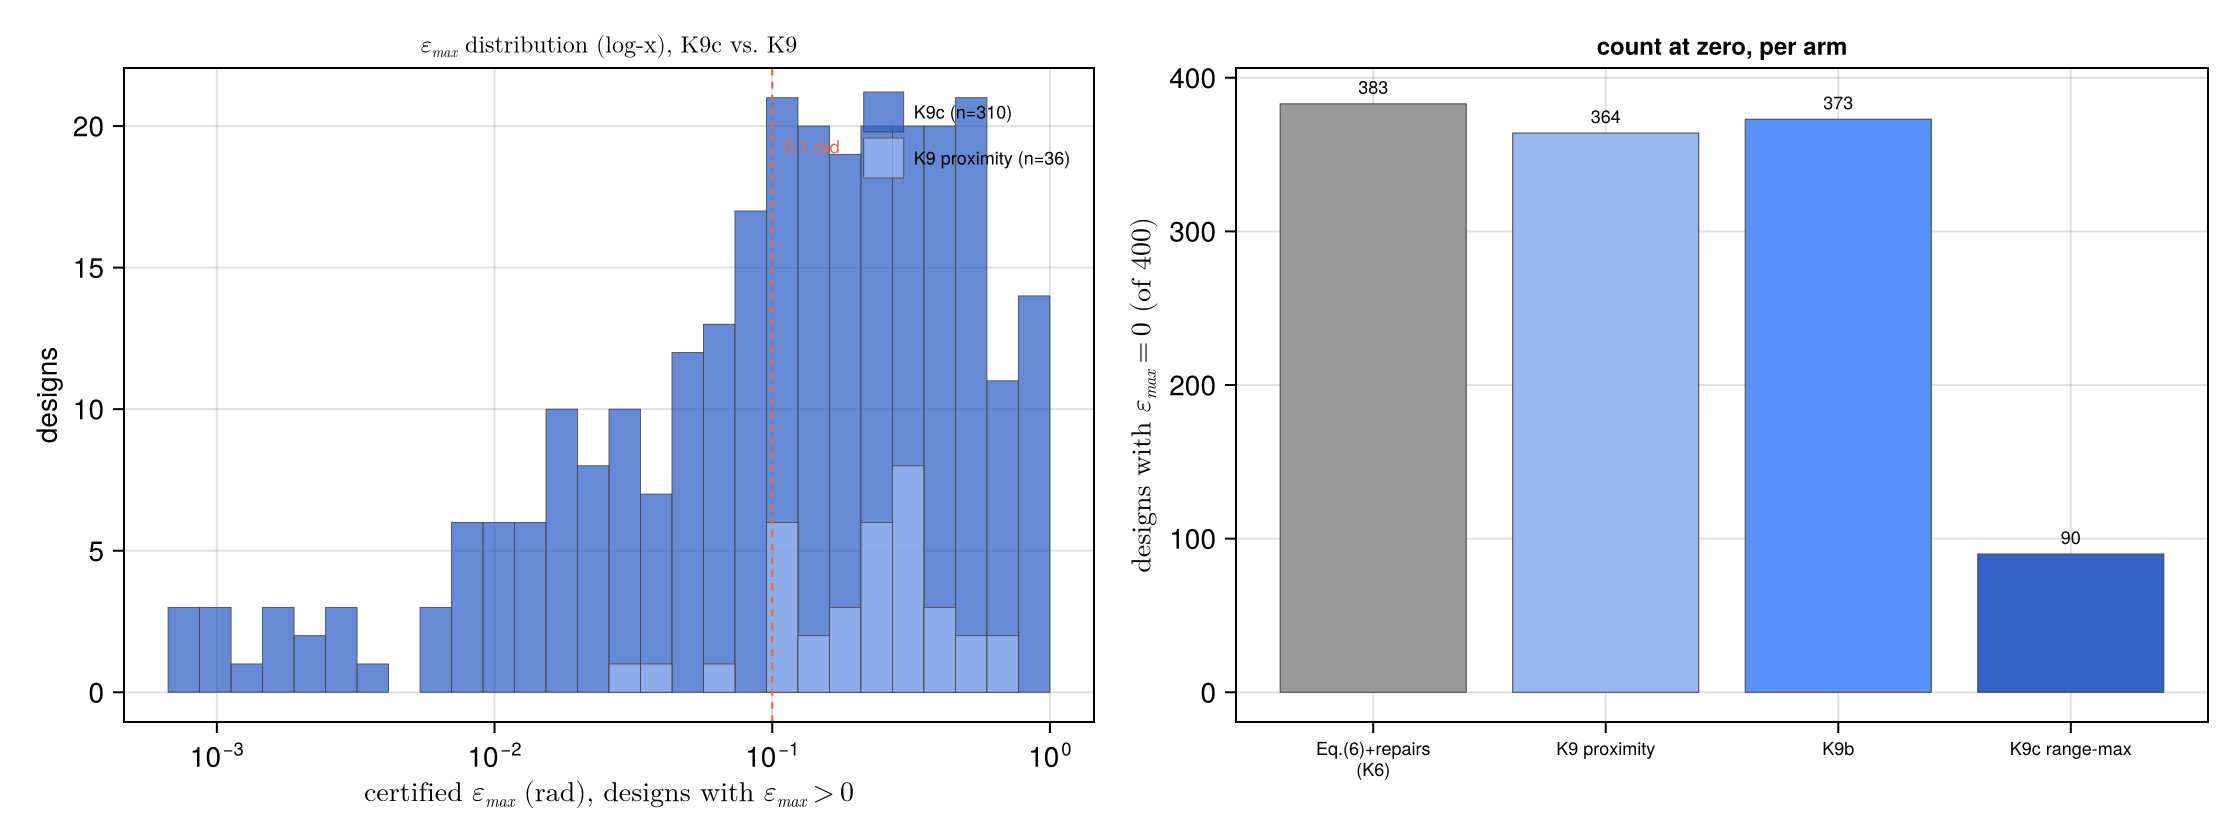
\includegraphics[width=0.70\textwidth]{../../results/final/figures/fig_eps_hist.png}
\caption{Distribution of the certified $\varepsilon_{\max}$ (log-$x$) for K9c against the K9
proximity arm, plus the count of zero-$\varepsilon_{\max}$ designs per arm.}
\label{fig:epshist}
\end{figure}

\clearpage
%==============================================================================
\section{Periodic patterns: the affine deployment Jacobian}
\label{sec:periodic}
%==============================================================================

The 2026 paper's §5.1 treats periodic patterns through the deployment Jacobian of the
fundamental parallelogram, and states one property ``empirically \dots for all $\theta$''.
This section derives that property, gives the achievable set exactly, adds a closed form the
paper does not state, and reports the constructive experiment that \emph{fails} for the same
$0^+$ reason as everything in Section~\ref{sec:diagnostics}.

\subsection{Why a genuine quotient, not a finite patch}

Judgement call 11 imposes the periodic identifications as linear constraints on a finite patch
whose boundary edges are \emph{not} topologically identified. Every hole preimage straddling
the seam of that patch then touches the mesh boundary, so by judgement call 2 it contributes
no row of $L$ --- and those are exactly the wrap-around deployability conditions. Those
conditions are what makes the face potential $u$ of Section~\ref{sec:kinematics} exist on the
infinite tiling, which is what makes the deployed structure periodic at all. So
\file{method/periodic\_jacobian.jl} builds the genuine quotient: one face per translation
class, edges keyed by (class pair, lattice offset), and hole rows carrying the integer offset
sum on the right-hand side. The lattice itself is detected by matching face centroids of equal
signature (side count plus sorted edge lengths) and taking the two shortest independent
self-translations. \textbf{[N]} The finite-patch $\dim\mathrm{null}$ is systematically larger:
\file{voronoi\_torus\_3\_n45} gives 45 on the quotient and 63 on the patch.

\subsection{C1: the Jacobian is affine, and the achievable set is an affine subspace}

\begin{theorem}[C1]
\label{thm:c1}
Let $u$ be the face potential. Translating the picture by a period $t$ gives
\[
u_{f+t} \;=\; u_f + w_t + \tfrac12\sigma_f t ,
\]
with $w_t$ \emph{constant over faces}, because the increment
$(\sigma_g-\sigma_f)t/2=\sigma_g t$ absorbs the shift of $x_{\mathrm{src}}$. Substituting into
\eqref{eq:T15}, the $\sigma_f t$ terms cancel and
\[
y_{(v+t,\,f+t)}(\theta) - y_{(v,f)}(\theta) \;=\; \cos(\theta/2)\,t + 2\sin(\theta/2)\,J w_t .
\]
Hence with $P_0=[t_h\ t_v]$ and $Q=2J[w_h\ w_v]$,
\begin{equation}
P_\theta = \cos(\theta/2)P_0 + \sin(\theta/2)Q,
\qquad
\boxed{\;J(\theta) = P_\theta P_0^{-1} = \cos(\theta/2)\,I + \sin(\theta/2)\,K,\quad K=QP_0^{-1},\;}
\label{eq:c1}
\end{equation}
with $K$ \textbf{constant in $\theta$} and \textbf{affine in the shape coordinate} ($P_0$ is
fixed data on the shape space). \textbf{[A]}
\end{theorem}

\noindent Consequently the achievable set $\mathcal{K}=\{K(X):X\in\mathbb{X}\}$ is an
\emph{affine subspace} of the $2\times2$ matrices, and inverse design of the whole
$\theta$-history reduces to \textbf{one linear solve}.

\textbf{[N] Verified, basis against independent forward kinematics} (33 patterns: seven
periodic families at $2\!\times\!2$, $3\!\times\!2$, $3\!\times\!3$ cells, plus 12 periodic
Voronoi tori of 20--200 faces per cell, $\sigma$ from Eq.~(1) solved as max-cut \emph{on the
quotient dual}):

\begin{center}
\small
\begin{tabular}{@{}lrr@{}}
\toprule
quantity & bar & worst over 33 patterns \\
\midrule
$\|P_\theta^{\mathrm{fit}}-P_\theta^{\mathrm{FK}}\|/\|P_\theta^{\mathrm{FK}}\|$, 50 angles & $10^{-9}$ & $\mathbf{1.37\times10^{-13}}$ \\
$\|K_{\mathrm{fit}}-K_{\mathrm{basis}}\|_\infty$ & $10^{-9}$ & $1.04\times10^{-13}$ \\
second difference of $t\mapsto K$ (affinity), 31 triples/pattern & $10^{-9}$ & $4.88\times10^{-14}$ \\
$\|P_0-T\|_\infty$ (measured period vs the lattice) & --- & $6.22\times10^{-14}$ \\
\bottomrule
\end{tabular}
\end{center}

\paragraph{The dimension formula is not the one we guessed.} The pre-registered spec expected
$\dim\mathcal{K}=\min(4,2\dim\mathrm{null})$. Measured:
\begin{itemize}\itemsep2pt
\item \textbf{$\dim\mathcal{K}=2\,\mathrm{rank}(D)$ on 33/33}, where $D$ is the $k\times2$
matrix of period-potential increments $w_t$. This is the formula, and it is exact.
\item $\min(4,2\dim\mathrm{null})$ \textbf{fails on 1/33}: \file{squares\_3x3} has
$\dim\mathrm{null}=4$ (6 split cuts) yet $\dim\mathcal{K}=0$, because its $K$ is frozen at a
\emph{rotation} ($\mathrm{tr}\,K=0$, $\det K=1$) over the entire 4-dimensional shape space ---
$J(\theta)$ is a rigid rotation by $\theta/2$ at every design and the cell never opens.
\end{itemize}
\textbf{Shape-space dimension does not bound designability; the rank of the period-potential
map does.} On 25 of the 33 patterns $\dim\mathcal{K}=4$, i.e.\ the map $t\mapsto K$ is
\emph{surjective} onto all $2\times2$ matrices. ($\dim\mathcal{K}=2\,\mathrm{rank}(D)$ is
currently \textbf{[N]}-only, verified on 33/33 but not derived; proving it is listed as open.)

\subsection{C2: conformal deployment is exact at every angle}

\begin{corollary}[C2 --- this settles 2026 §5.1's ``empirically'']
\label{cor:c2}
$J(\theta)$ is a similarity for \emph{every} $\theta$ if and only if $K$ is one. \emph{Proof.}
The similarities are the linear span of $\{I,J\}$, and by \eqref{eq:c1} $J(\theta)$ is an
affine path through $I$ in the direction $K$; an affine path through a point of a linear
subspace stays in the subspace iff its direction lies in it. \hfill$\square$
\end{corollary}

\noindent The paper's Eq.~(13) imposes the two linear conditions
$\partial_\theta(J_{11}-J_{22})|_0=0$ and $\partial_\theta(J_{12}+J_{21})|_0=0$ and then
observes that ``once the derivative of the conformal distortion vanishes at $\theta=0$, the
deployment remains conformal for all opening angles''. Corollary~\ref{cor:c2} is a one-line
proof of that sentence, given C1, and turns an admitted empirical gap into a theorem.

\textbf{[N]} On all \textbf{25} patterns with $\dim\mathcal{K}\ge1$ the two linear
conformality equations ($K_{11}=K_{22}$, $K_{12}=-K_{21}$) are consistent to residual
$\le\mathbf{9.67\times10^{-17}}$, and at the solution the conformal distortion of $J(\theta)$
over \textbf{200 angles spanning $[0,\pi]$} is $\le\mathbf{2.31\times10^{-14}}$ (best:
\file{hexagons\_2x2}, $1.76\times10^{-16}$).

\subsection{C4: the closed form for the second fully-closed angle}

\begin{proposition}[C4]
The void area per cell is $A(\theta)=\det(P_0)\,(\det J(\theta)-1)$. Substituting
\eqref{eq:c1} and the half-angle identities gives the first harmonic
$A(\theta)=q(\cos\theta-1)+r\sin\theta$ with
\[
q = -\tfrac12\det(P_0)\,(\det K-1),\qquad
r = \tfrac12\det(P_0)\,\mathrm{tr}\,K,
\]
so, since $\det P_0$ cancels,
\begin{equation}
\boxed{\;\theta_c \;=\; 2\,\mathrm{atan2}\bigl(\mathrm{tr}\,K,\; 1-\det K\bigr).\;}
\label{eq:thetac}
\end{equation}
Note $p+q=0$ automatically, so $\theta=0$ is always a root; the second root is the content.
\textbf{[A]}
\end{proposition}

\textbf{[N]} Worst $|\theta_c-\theta_{\mathrm{measured}}|$ (bisection on the forward-kinematics
hole area): $\mathbf{5.53\times10^{-14}}$ on 32 periodic patterns and
$\mathbf{4.44\times10^{-16}}$ on 7 bounded patches, against a bar of $10^{-6}$. The one
excluded periodic row is \file{squares\_3x3}, which has $q=r=0$ so $A\equiv0$ and there is no
second closed state --- consistent with $K$ being a rotation. On the bounded patches the
closed state is overlap-free ($\theta_c\le\Tmax$) on \textbf{4/7}: \file{rotating\_squares}
($\pi$), \file{kagome\_3636} ($\pi$), \file{hexagons\_auto} ($2\pi/3$),
\file{truncated\_square\_488} ($3\pi/4$); it is unreachable on
\file{triangles\_alternating} ($\theta_c=4\pi/3>\pi$), \file{snub\_square\_33434}
($3.768$ vs $\Tmax=1.646$) and \file{tiling\_3\_4\_3\_12} ($2.818$ vs $2.381$).
\emph{Predicting the angle is exact; reaching it is a separate and often negative question.}

\subsection{C3: target-driven design fails, for the same \texorpdfstring{$0^+$}{0+} reason}

Since $\mathcal{K}$ is an affine subspace, a target $K^*$ can be hit by least squares and the
leftover freedom spent maximising certified $\Tmax$. Bar: $\ge80\%$ of patterns with
$\dim\mathcal{K}\ge1$ hit the target to $<10^{-8}$ \emph{with a certified, $\Tmax>0$ design}.

\begin{center}
\small
\begin{tabular}{@{}lrrrr@{}}
\toprule
target & patterns & max hit error & $0^+$ feasible & \textbf{certified $\Tmax>0$} \\
\midrule
random $K^*\in\mathcal{K}$ & 25 & $\mathbf{8.88\times10^{-16}}$ & 21/25 & \textbf{12/25 (48\%)} \\
anisotropic $K^*=\mathrm{diag}(1,-0.5)$ & 25 & $8.88\times10^{-16}$ (24) / $1.0$ (1) & \textbf{0/25} & \textbf{0/25} \\
\bottomrule
\end{tabular}
\end{center}

\noindent \textbf{Verdict: FAIL, 48\% against 80\%. Reachability is never the problem.} On 24
of 25 patterns even the anisotropic target is hit to $8.9\times10^{-16}$, because
$\dim\mathcal{K}=4$ makes $\mathcal{K}$ the whole matrix space. The single genuinely
unreachable case is \file{squares\_3x2}, the only pattern with $\mathrm{rank}(D)=1$, whose hit
error is exactly $1.0$. Every other failure is the \emph{same $0^+$ obstruction}: the design
realising $K^*$ places at least one split cut so that its two duplicates translate into each
other, $\min_e q_e<0$, and $\Tmax=0$ before any certificate is consulted. On
\file{snub\_square} and \file{t3\_4\_3\_12} the anisotropic design overshoots by
$\min q\approx-42$ to $-46$, two orders past the boundary; on hexagons, 4.8.8 and Voronoi the
overshoot is $O(1)$ and sometimes only $-0.22$, so those are where a margin-aware search might
still recover a design.

\paragraph{Why this is the strongest evidence in the whole campaign.} K7 reproduces the $0^+$
obstruction on a population sharing \textbf{nothing} with the construction of
Section~\ref{sec:diagnostics}: periodic instead of fixed-boundary, tori instead of random
Delaunay patches, tilings as well as random Voronoi. A negative result reproduced across
independent generators is worth more than another positive on the same one.

\paragraph{Where a design \emph{is} certified, the closed form is right.} Over the 12 certified
designs the largest discrepancy between the predicted Poisson-ratio curve $\nu(\theta)$ from
$K$ and forward kinematics, at 20 angles and 2 directions, is $\mathbf{9.13\times10^{-11}}$,
and both the certified $\varepsilon$ and the exact $\Tmax$ reach $2.32$ rad
(\file{t3\_4\_3\_12\_3x2}).

\paragraph{Two anomalies, both chased down.} (i) The area-harmonic fit error over a full
$\theta\in(0,2\pi)$ sweep is $10^{-15}$ on the 21 tilings but reaches $2.3\times10^{-2}$ on
the Voronoi tori. It is \emph{not} a failure of the harmonic: the deviation is localised
exactly to the interval where $\det P_\theta<0$ --- the deployed cell has inverted --- and is
an artefact of the measurement using $|\det P_\theta|$ where the harmonic is the \emph{signed}
$\det P_0(\det J-1)$. Off that interval the agreement is $10^{-15}$ at every sampled angle.
(ii) The per-corner period consistency statistic is $\le1.1\times10^{-13}$ on 32/33 patterns
and \textbf{27.5} on \file{snub\_square\_3x3}, whose cut structure has 9 connected components,
each threading all 9 cell copies; \file{deploy()} gauges each component independently, so the
period read from different components differs by a gauge offset growing with $\theta$.
\textbf{\file{snub\_square\_3x3}'s $K$ is gauge-dependent and must not be quoted}; removing it
changes none of the worst-case figures above, because it is never the maximum in any of them.

\begin{figure}[t]
\centering
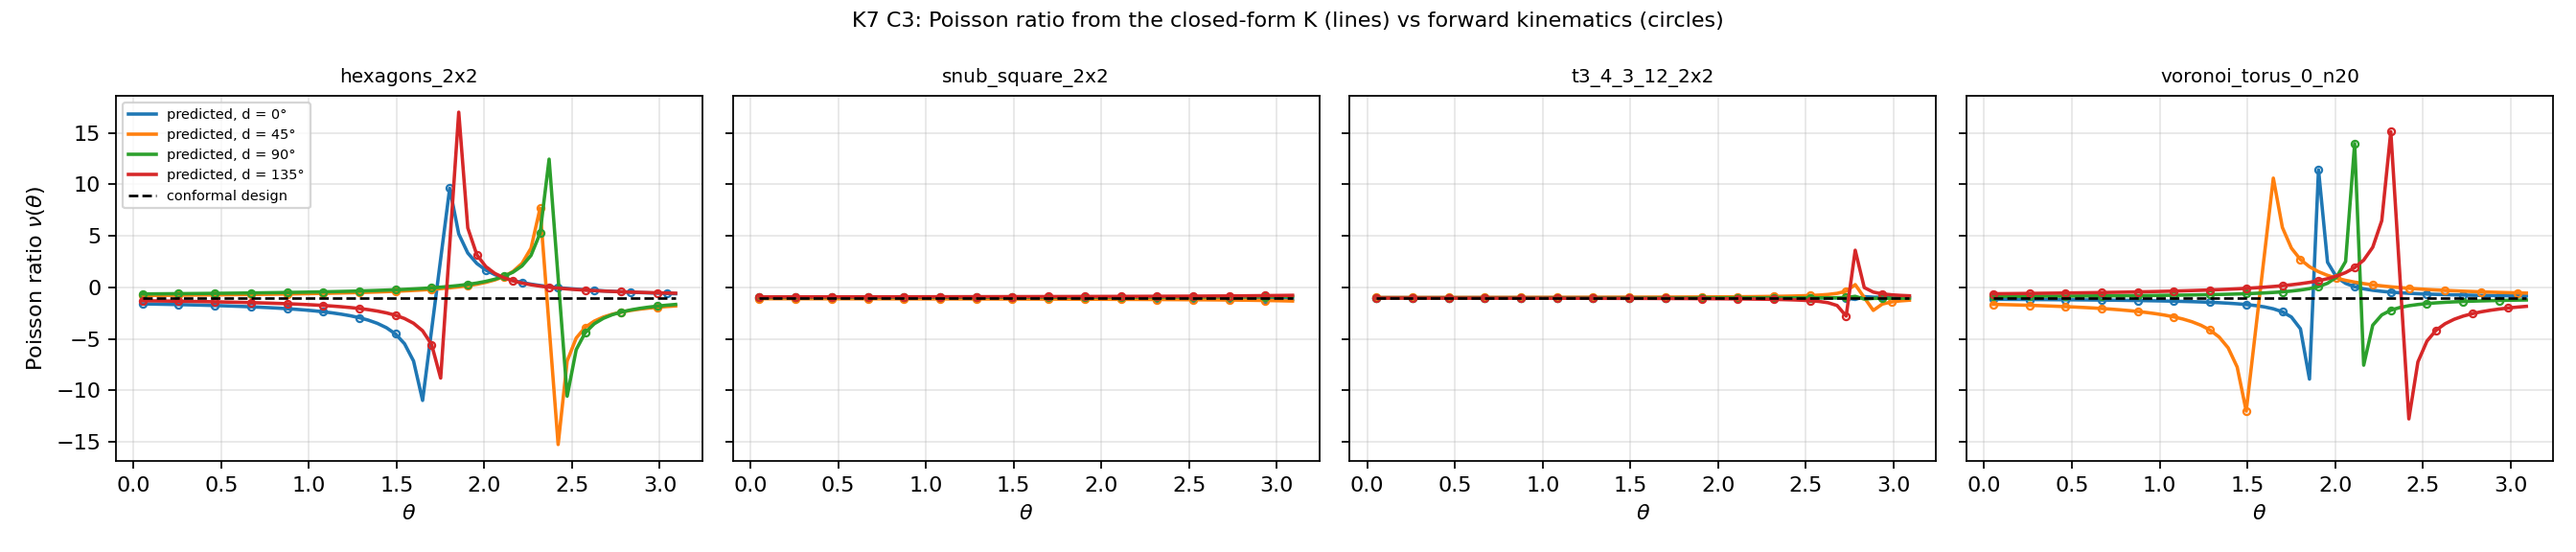
\includegraphics[width=0.48\textwidth]{../../results/kill/k7/k7_nu_curves.png}\hfill
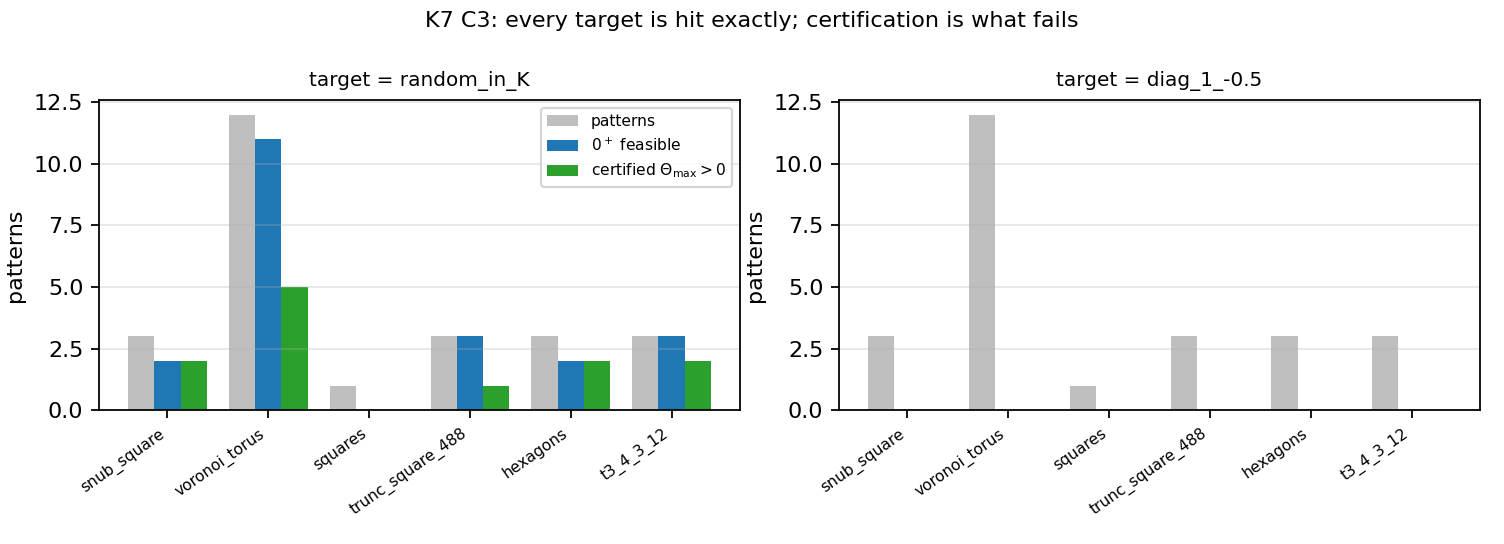
\includegraphics[width=0.48\textwidth]{../../results/kill/k7/k7_c3_certified.png}
\caption{Left (C3): predicted Poisson-ratio curves $\nu(\theta)$ from $K$ (lines) against
forward kinematics (circles) on four patterns, with the conformal design as the flat dashed
curve. Right (C3): per family, the number of patterns, the $0^+$-feasible count and the
certified count --- reachability is total, the $0^+$ collision is the obstruction.}
\label{fig:k7}
\end{figure}

\subsection{F35: the hole-area harmonic, and the budget that fails as an algorithm}

\begin{proposition}[per-hole area is a first harmonic]
For a hole preimage $C$, $A_C(\theta) = a_C\sin\theta - b_C(1-\cos\theta)$ with
$a_C=\tfrac12\sum_{\partial C}\langle x_a-x_b,u_f\rangle$ and
$b_C=\tfrac12\sum\sigma_f\det(\cdot)$; the max-area angle is $\tfrac12\theta_c(C)$ with
$\theta_c(C)=2\,\mathrm{atan2}(a_C,b_C)$. \textbf{[A]}, a direct corollary of
Theorem~\ref{thm:t3} applied to the shoelace area.
\end{proposition}
\noindent\textbf{[N]} $8.7\times10^{-14}$ over 471 holes on 10 patterns; the total void area
equals a border functional to $3.41\times10^{-15}$ at 6 angles, and the edge-wise budget
satisfies $W+R=2B(X)$ to $2.74\times10^{-16}$ on 10 patches. Notches are not a correction but
a real effect: $\sum_C a_C$ is 34--45\% \emph{below} the hole-only sum on every pattern, i.e.\
notches close as holes open.

\paragraph{The periodic identity needed a repair, and the repair changes what it says.} Both
copies of an edge contribute $\langle x_a-x_b,\,u_{f_1}-u_{f_0}\rangle$. For a split edge
$\sigma_{f_0}=\sigma_{f_1}$ and the term is lattice-translation invariant; for a hinge edge
$\sigma_{f_0}=-\sigma_{f_1}$ and
$u_{f_1+t}-u_{f_0+t}=u_{f_1}-u_{f_0}+\sigma_{f_1}t$, so the term depends on \emph{which lift}
the preimage walk uses. Summing one arbitrary representative per quotient \emph{edge} misses a
defect measured at $0.38$--$1.88\times\det P_0$ on the 33 patterns. Summing one representative
\emph{preimage} per translation class, each at its own lift, gives
\begin{equation}
W + R \;=\; \det P_0\cdot\mathrm{tr}\,K
\label{eq:budget}
\end{equation}
to $10^{-15}$ on 30 of 33 patterns and 46 of 50 target-design rows (the exceptions are
\file{squares\_3x2}, whose super patch carries no full representative set, and
\file{snub\_square\_3x3}, the gauge-dependent one). Consequently
$\mathrm{tr}\,K-\tau^* = R/\det P_0$ \emph{exactly}: the budget gap \textbf{is} the total split
budget rescaled, $\tau^*$ is a function of the design rather than of the pattern, and
$\mathrm{tr}\,K\ge\tau^*$ is \emph{not} a linear constraint on the achievable set.

\paragraph{And the algorithm built on it fails, by its own pre-registered hard-fail clause.}
As a \emph{predictor} the quantity is excellent: AUC$(\mathrm{tr}\,K-\tau^*)$ is
\textbf{0.980} for $\min q>0$ and \textbf{0.950} for certified, against a bar of 0.80, with
\emph{zero} rows having $\min q>0$ at $\mathrm{tr}\,K<\tau^*$. But the hard-fail clause fires:
$\mathrm{spread}(W)/\mathrm{spread}(\det P_0\,\mathrm{tr}\,K)$ over $\mathcal{K}$ has median
\textbf{0.727} and max \textbf{1.401} --- \emph{$W$ moves as much as the budget}, so $\tau^*$
is a penalty, not a threshold. The constrained re-solve confirms it: certified
$12\to13$ ($\delta=0$), $12\to14$ ($\delta=0.1$), $12\to2$ ($\delta=0.5$), all inside the
50-row binomial error bar of $\pm4.6$, while $\min q>0$ rises $21\to37$ and the target is
abandoned (isotropic correction $10$--$589$ in Frobenius norm). The identity survives as a
verified theorem; the design principle does not, and \textbf{the identity must not be cited in
support of a design algorithm the same document kills}.

\clearpage
%==============================================================================
\section{Baselines, and the fairness of every comparison}
\label{sec:baselines}
%==============================================================================

Every ``0/400'' in this report needs to say precisely \emph{whose} pipeline produced the
zero. This section makes that explicit, reports the one comparison in which the authors' code
outperforms ours, and states the caveats that a careful reader will and should raise.

\subsection{K2b: our range optimiser does not beat their native \texttt{prevent}}

Baseline: \file{tuttekiri\_cli prevent --sweep}, starting from \emph{their} Eq.~\eqref{eq:eq6}
projection and running \emph{their} \file{opt::prevent\_intersections}, with the full 84-point
parameter grid on the four reference cases and a 36-point sub-ladder elsewhere (which contains
the published default $(0.1,10,0.1)$ and every corner of the full grid). Their own
$\theta_{\max}$ is never used (it fuses hinge duplicates before testing). Referee: our
bisection on the true polygon overlap, 4{,}000-point grid, applied identically to every ladder
point; a ladder point counts only if it is a valid flat embedding.

\begin{center}
\small
\begin{tabular}{@{}lrl@{}}
\toprule
quantity & value & rule \\
\midrule
designs & 38 (30 live, 8 vacuous) & \\
\textbf{median relative gain over the native baseline} & \textbf{0.0000} & $\ge0.25$ \ding{55} \\
designs with certified validity and range $>0$ & 30 / 38 & $\ge20$ \ding{51} \\
ours better / native better / tie & \textbf{7 / 15 / 16} & \\
gain quartiles over the 30 live designs & $-0.305,\,-0.018,\,0.000,\,0.000,\,+0.106$ & \\
snub square & native $3.1416$, ours $3.1416$, $\min\beta=3.3839$ & gap closed $0.0\%$ \ding{55} \\
\bottomrule
\end{tabular}
\end{center}

\noindent \textbf{Verdict: FAIL, on both clauses, and not narrowly.} Three honest readings:
\begin{itemize}\itemsep2pt
\item \textbf{The authors' code is strong.} On \file{snub\_square\_33434} their ladder reaches
$\Tmax=\pi$ --- the top of the search range --- certified by our own bisection. There is no
headroom left to win. An earlier internal figure of ``86.1\% gap closure'' was measured
against \emph{our} $X_0$ ($1.6461\to\pi$), not against their code; against their code the gap
is already closed and our number is a tie. That figure is withdrawn.
\item \textbf{Our optimiser mostly does not move.} On 16 of 30 live designs it returns exactly
the refereed range it started from. Where we lose we lose badly (\file{hexagons\_R20\_s5/s6}:
native $3.0148$ and $2.9530$, ours stuck at $2.0944=2\pi/3$, the graze-limited hexagon value
--- our optimiser sits at the local barrier while their penalty walks the design out of the
hexagon geometry entirely). Where we win we win little: best $+10.6\%$.
\item \textbf{The random graphs make the experiment vacuous, which is itself the finding.} On
eight random graphs, \textbf{0 of 37} native ladder points is a valid flat embedding. Baseline,
our Eq.~(9) and our optimiser all return $\Tmax=0$ and the relative gain is $0/0$. This is the
emptiness result reappearing with the authors' own code.
\end{itemize}
\noindent Consequence: any range-\emph{margin} claim is dead and was dropped. What survives is
the diagnostic half, and later the constructive half of Section~\ref{sec:rangeembed}, whose
comparison is against a baseline of zero rather than against a margin.

\subsection{Native200: their full pipeline, run unconditionally}

Every earlier comparison against the authors' code was capped --- K2b on 30 live designs,
K6's side-run on the 8 of 400 designs that reached a valid flat state. Neither is their
\emph{full} pipeline (their own colouring, their Eq.~(6), their Eq.~(9), their collision test)
run \emph{unconditionally}, with no pre-filter, on the same 200-graph population. This is that
run, and it exists precisely because a reviewer would otherwise say ``you never actually ran
our optimiser on your graphs''.

\noindent\textbf{Native baseline, not rerun.} Every number from the authors' pipeline (this section,
the K2b ladders, the \texttt{native} cells of the regime study) comes from their unchanged binary
(\file{baseline/native/}, \file{tuttekiri\_cli}) and is reused as archived; the Julia port reruns
our side only.

Three variants per graph --- \emph{native} (their own colouring), \emph{sigma\_mc}, and
\emph{sigma\_def} --- each wrapped in a 600 s alarm, so a cell is \texttt{completed},
\texttt{timed\_out} or \texttt{crashed}. The returned embedding is re-evaluated with
\emph{our} instruments: the exact scan, the bisection referee, and the $\varepsilon=0.3$
certificate; their own collision output is recorded only as a diagnostic column.

\begin{center}
\small
\begin{tabular}{@{}lrrrr@{}}
\toprule
 & \texttt{native} & \texttt{sigma\_mc} & \texttt{sigma\_def} & total \\
\midrule
completed & 57 & 64 & 51 & \textbf{172} \\
timed out & 130 & 123 & 109 & \textbf{362} \\
crashed & 2 & 6 & 31 & \textbf{39} \\
dispatched & 189 & 193 & 191 & 573 \\
\bottomrule
\end{tabular}
\qquad
\begin{tabular}{@{}lrrr@{}}
\toprule
family & completed & timed out & crashed \\
\midrule
delaunay & 118 & 66 & 8 \\
voronoi & 41 & 147 & 5 \\
quad\_random & 13 & 149 & 26 \\
\bottomrule
\end{tabular}
\end{center}

\noindent \textbf{[N] Result on the 172 completed cells.} Their own collision test reports
$\Theta>0$ on \textbf{5}; our exact scan on the \emph{same} dumped embedding gives $\Tmax>0$
on \textbf{0 / 172}; the certificate holds on \textbf{0 / 172}. All five apparent positives
fail $\POS$, and the exact scan finds an immediate $0^+$ contact that their
\file{merge\_close\_verts} fuses away before their test ever sees it --- the same F24/K1c
mechanism, now measured unconditionally rather than on a hand-picked set.

\begin{center}
\small
\begin{tabular}{@{}rlllrrrrr@{}}
\toprule
id & kind & variant & & $|F|$ & $\dim\mathrm{null}$ & native $\Theta$ & our exact & our bisect \\
\midrule
160 & delaunay & native & & 292 & 59 & 0.0880 & 0.0000 & 0.0000 \\
36 & voronoi & sigma\_def & & 131 & 235 & 0.6726 & 0.0000 & 0.0000 \\
102 & voronoi & sigma\_def & & 336 & 600 & 0.3508 & 0.0000 & 0.0000 \\
168 & voronoi & sigma\_def & & 138 & 238 & 1.0248 & 0.0000 & 0.0000 \\
156 & voronoi & sigma\_def & & 308 & 566 & 0.5704 & 0.0000 & 0.0000 \\
\bottomrule
\end{tabular}
\end{center}

\paragraph{The caveat, stated as strongly as a critic would.} This run is \textbf{partial}: it
was stopped by the user at 573 of 600 cells, and it is $0\%$ \emph{of what finished}. Timeouts
dominate (63\%) and are concentrated where $|F|$ is largest --- median $|F|$ is 202 for
completed cells against 490.5 for timed-out ones and \textbf{332.5} for the population, versus
$\le97$ for the 2026 paper's own worked examples. \file{quad\_random} is worst hit: 149/188
timed out and 26/188 crashed. The crash cause was reproduced afterwards (\file{STATE.md} F42):
an empty-vertex-list access in \file{convert::to\_eig\_mat}, reached from
\file{Hmesh::merge\_close\_verts} once a deployed configuration has collapsed to zero faces,
not the unchecked \file{prev()->twin()} in \file{get\_holes()} that the original F24 note
assumed --- that null dereference is real but latent, and the same patch
(\file{results/kill/native200/crashfix.patch}) fixes both. So the honest reading has two halves, and both belong
in any quotation of this number: their pipeline does not escape the $0^+$ jam on the designs
where it finishes, \emph{and} its practical operating range on this hardware is smaller graphs
than this population supplies --- which is itself informative about scaling, independently of
the obstruction. Finishing the last 27 runs would change nothing qualitatively; rerunning the
362 timeouts with a longer budget is the one remaining item.

\subsection{Population caveats, collected}

\begin{enumerate}\itemsep3pt
\item \textbf{The papers never claim random graphs.} The 2026 generality claim is
\emph{combinatorial}: ``our analysis applies to arbitrary planar graphs, including those that
are non-periodic, non-2-colorable, or with inner holes'', demonstrated with one hand-picked
example per exclusion. No figure, table or sentence reports a success rate over a
\emph{population} of any kind. The random-graph experiment is entirely ours, and the framework
cannot be shown to overclaim on a question it never poses. Every ``0/400'' in this report is a
statement about what \emph{we} measured on \emph{our} population.
\item \textbf{Scale.} $|F|\in[101,793]$, median $332.5$, against $|F|\in[4,97]$ for every
reference case in the papers' figures. The generative process is unbiased; the scale is
outside what is demonstrated. Both are true.
\item \textbf{Half the authored controls are trivial.} Four of the eight reference tilings are
split-free, so their shape space is a single point and they pass by construction
(Section~\ref{sec:diagnostics}). ``Authored tilings pass 8/8'' means ``4 trivially, 4
substantively''.
\item \textbf{Which certificate produced which number.} Early experiments (K1a, K2b, K1c, and
K5's comparison row) used a $\theta=0$ overlap predicate that has since been
\textbf{withdrawn} as degenerate. Those numbers are quoted \emph{as they were measured} and are
not restated under the corrected certificate; where the two disagree, the disagreement is the
finding and both are printed.
\item \textbf{Rank estimates above $\approx700$ columns are unreliable.} On 15 of 508 graphs
\file{SparseQR} gives a rank wrong by exactly $\pm1$ where the singular gap is
$5.9\times10^{-5}$ to $1.7\times10^{-3}$ --- three to eight orders above the threshold, so it
is not a borderline call. Seven of seven violators small enough for a dense QR have the
identity restored \emph{exactly}. \textbf{No rank above 700 faces is quoted} without a dense
recheck, and every mobility number inherits this caveat.
\item \textbf{Mobility is not a dangling-face artefact.} After 2-core reduction, Delaunay
mobility is still median \textbf{305} (range 36--1675) and the pre-registered clause
$m_{\mathrm{core}}\le5$ holds on \textbf{0 of 167} patches. The 2-core identity
$\dim\ker A = |F\setminus\mathrm{core}_2| + \dim\ker A|_{\mathrm{core}_2}$ holds on 493/508 as
measured, with every exception off by exactly $\pm1$ and 7/7 dense rechecks exact.
\item \textbf{A Gate-2 artefact that must be labelled.}
\file{results/core\_validation/reference\_cases.md} reports snub-square $\Tmax=1.646$ from the
\emph{old} collision code plus bisection; T4's exact value is $1.671$. Different code eras,
not different seeds. The T4/K2a numbers are authoritative.
\end{enumerate}

\clearpage
%==============================================================================
\section{Software}
\label{sec:software}
%==============================================================================

Everything is Julia ($\geq 1.10$), one package \file{Kirigami}. Python appears only for matplotlib plotting of CSV/JSON
dumped by the Julia apps. Dependencies are the standard library (\file{LinearAlgebra}, \file{SparseArrays},
\file{Random}, \file{Statistics}, \file{Printf}) plus \file{StaticArrays} ($\mathbb{R}^2$ vectors), \file{JSON} (I/O) and
\file{DelaunayTriangulation} (random-point generators); the L-BFGS with backtracking line search is ours, so there is
no external optimiser anywhere in the pipeline. Dense factorisations are \file{LinearAlgebra} (\file{qr(A, ColumnNorm())},
\file{svd}), sparse ones \file{SparseArrays}/SuiteSparse; \file{std::mt19937} is ported bit-exactly (\file{core/mt19937.jl}).

The authors' baseline is not part of the package: \file{baseline/native/} is their unchanged C++
(libigl, Optiz, Eigen~3.4), and every ``native'' number in this report (Native200, K2b, the regime
study's native cells) is reused as archived rather than rerun.

\subsection{Build and test}

\begin{verbatim}
julia --project=Kirigami -e 'using Pkg; Pkg.instantiate()'   # one-off
julia --project=Kirigami -e 'using Pkg; Pkg.test()'          # ⟨JULIA:tests⟩, 0 failures; includes derivation_tests.jl (⟨JULIA:derivation\_tests⟩)
\end{verbatim}

\noindent Both counts were re-run for this report and are the numbers reported, not copied
from an earlier log. \file{derivation\_tests} is a \emph{standalone} suite written by the
independent Checker against the derivation, not by the implementer against the code; it is the
cross-check for every theorem in Sections~\ref{sec:kinematics}--\ref{sec:certificate}.

\subsection{Repository map}

\begin{center}
\small
\begin{tabular}{@{}p{0.30\textwidth}p{0.62\textwidth}@{}}
\toprule
area & path \\
\midrule
core pipeline (2026 reimplementation) & \file{Kirigami/src/core/}: \file{mesh} \file{cut} \file{holes} \file{orientation} \file{tutte\_auxetic} \file{kinematics} \file{collision} \file{optimize} \file{rank\_checks} \file{generators} \file{import\_soup} \file{mt19937} \\
method layer & \file{Kirigami/src/method/}: \file{deploy\_basis} \file{contact} \file{design} \file{range\_opt} \file{zero\_plus} \file{convex\_embed} \file{range\_embed} \file{mobility} \file{expansive\_cone} \file{periodic\_jacobian} \file{budget} \\
fabrication export & \file{Kirigami/src/export/}: \file{layout} \file{solid} \file{svg} \file{stl} \file{threemf} \file{xml} \file{zip} \file{material} \\
tests & \file{Kirigami/test/}: \file{test\_mesh\_cut} \file{test\_holes} \file{test\_system} \file{test\_kinematics} \file{test\_collision} \file{test\_method} \file{test\_design} \file{test\_range\_embed} \file{test\_rank\_checks} \file{test\_reference\_cases} \file{test\_export} \file{test\_import\_soup} \file{test\_mt19937} \file{derivation\_tests} \\
CLIs & \file{Kirigami/apps/}: \file{kiri\_gen} \file{kiri\_analyze} \file{kiri\_deploy} \file{kiri\_design} \file{kiri\_export} \file{kiri\_sweep} \file{kiri\_reference} \\
experiment drivers & \file{Kirigami/apps/kill\_*}: \file{k1a} \file{k1b} \file{k1c} \file{k2a} \file{k2b} \file{k2c} \file{k3a} \file{k5} \file{k6} \file{k7} \file{k8a} \file{k9} \file{k9b} \file{k9c} \file{b3} \file{b4} \file{t1} \file{jitter} \file{e1} \file{native200} \file{f23} \\
frozen corpora & \file{data/corpus/}: the graph populations every driver reads (produced once, never regenerated) \\
desktop explorer & \file{Kirigami/gui/}: \file{app.jl} (GLMakie) \\
derivations & \file{derivations/core.md}, \file{derivations/check.md} \\
results & \file{results/kill/}, \file{results/final/}, \file{results/core\_validation/} \\
authors' code and parity & \file{baseline/native/}, \file{baseline/parity.md} \\
\bottomrule
\end{tabular}
\end{center}

\subsection{The JSON contract}

One interchange format for every tool, so payloads can be moved between the CLI, the tests and
the desktop explorer and compared byte for byte:

\begin{verbatim}
{ "vertices":    [[x, y], ...],           // 2D positions, one per vertex
  "faces":       [[i0, i1, ...], ...],    // simple polygons, CCW in the given geometry
  "orientation": [1, -1, ...],            // optional sigma per face: +1 = CW, -1 = CCW
  "periodic": { "th": [tx,ty], "tv": [tx,ty],
                "pairs_h": [[p,p'],...], "pairs_v": [[q,q'],...] } }
\end{verbatim}

\noindent Faces stored clockwise are silently reversed on load, because the
$\sigma$-to-direction rule is defined relative to the geometric CCW order. An edge shared by
more than two faces is rejected with an error. Deployment dumps use a second format carrying
\texttt{theta}, \texttt{max\_mismatch}, the $\Mprime$ vertices and faces, and one cycle per
hole.

\subsection{The method API}

\file{method/design.jl} is the single entry point, so that ``certified'' means one thing
across the library, the CLI and this report.

\begin{center}
\small
\begin{tabular}{@{}p{0.34\textwidth}p{0.58\textwidth}@{}}
\toprule
call & what it does \\
\midrule
\file{characterize(mesh,$\sigma$,X)} & exact $\Tmax$ by Theorem~\ref{thm:t422}, the complete contact list, and $\POS\wedge\NOOV(\varepsilon/2)\wedge\NOROOT(\varepsilon)$ with the largest certifiable $\varepsilon$ \\
\file{design\_range\_max(...)} & \textbf{the deliverable}, Algorithm~\ref{alg:k9c}: stage A then stage B from three starts, best of the arms, with \texttt{provenance} \\
\file{design\_constrained(...)} & the older K9 proximity embedding \eqref{eq:k9} \\
\file{design\_baseline(...)} & the Eq.~\eqref{eq:eq6} projection alone ($t=0$), characterised by exactly the same code \\
\file{orientation\_maxcut / \_defect} & the Eq.~(1) $\sigma_{\mathrm{mc}}$ and K5's $\sigma_{\mathrm{def}}$ \\
\bottomrule
\end{tabular}
\end{center}

\noindent \texttt{Characterization} carries \texttt{theta\_max}, \texttt{zero\_range},
\texttt{contacts}, \texttt{first\_contact}, \texttt{eps\_max}, the full certificate, and ---
when $\Tmax=0$ --- \texttt{binding}, the classification of what stops it
(\texttt{split-inward}, \texttt{inverted}, \texttt{vertex-edge}, \texttt{hinge-wedge}).
\texttt{CharacterizeOptions::referee} additionally runs the independent bisection as a
\textbf{cross-check}; it is not ground truth (Section~\ref{sec:diagnostics}, F34).

\paragraph{Baselines are characterised by the same code as the method.} \file{design\_baseline}
exists so that the ``0'' in every baseline row is produced by \emph{exactly} the routine that
produces the method's positives. That is the single most important property of this API for
the credibility of the comparison.

\subsection{Command-line usage}

\begin{verbatim}
# generate a graph, orient it, and analyse the whole pipeline
kiri_gen delaunay 400 --out g.json --seed 1 --orient auto
kiri_analyze g.json --orient json --boundary fixed --out results/tmp --collision

# the deliverable on one graph, both orientation rules, with the referee
kiri_design g.json --sigma both --out design.json --referee

# reproduce the hero exactly (10210 = 9300 + 7*130)
kiri_design export/hero2/hero2_input.json --sigma json --seed 10210 --out design.json
\end{verbatim}

\noindent Every run prints the winning arm and the whole candidate list, so provenance is
visible without opening the JSON:

\begin{verbatim}
sigma_json range_max : Theta_max = 3.141593 rad, eps_max = 3.141593 rad, certified = yes,
                       feasible = yes (min cross 8.996e-02, min q 1.240e-01 med^2),
                       inverted faces 0, winning arm = k9c/x0+B (stage B improved it)
    arm k9:       Theta_max = 0.332464, m = 4.959e-02, feasible = yes
    arm k9b:      Theta_max = 0.009498, m = 1.034e-02, feasible = yes
    arm k9c/k9:   Theta_max = 0.277041, m = 1.944e-01, feasible = yes
    arm k9c/k9b:  Theta_max = 0.136687, m = 1.920e-01, feasible = yes
    arm k9c/x0:   Theta_max = 0.278991, m = 1.915e-01, feasible = yes   <- stage A winner
    arm k9c/x0+B: Theta_max = 3.141593, m = 1.240e-01, feasible = yes
\end{verbatim}

\noindent \file{--sigma} selects \texttt{json} / \texttt{mc} / \texttt{def} / \texttt{both};
\file{--proximity} selects the older K9 solve and \file{--baseline} additionally reports the
Eq.~(6) projection. Shared knobs \file{--eps}, \file{--delta}, \file{--split-delta},
\file{--iters}, \file{--seed}, \file{--referee} apply to whichever method runs; K9c-only knobs
are \file{--delta-wide}, \file{--stages}, \file{--stage-iters}, \file{--no-stage-b},
\file{--no-arm-k9}, \file{--no-arm-k9b}. \file{--out-graph} writes the best design as a plain
graph JSON, which \file{kiri\_analyze}, \file{kiri\_deploy} and \file{kiri\_export} read
directly.

\subsection{Fabrication export}

\file{src/export/} turns an oriented graph into an SVG in millimetres and a 3D solid as binary
STL and 3MF. Everything fabrication-related lives in one \texttt{MaterialProfile} (thickness,
kerf, hinge type, neck width, pad radius, gap, minimum feature size, pin clearance); the
writers never hard-code a dimension. \texttt{face\_inset() = gap/2 + kerf/2} is the amount
every face is pulled back from each \emph{cut} side, so two faces of a cut edge end up
\texttt{gap} apart once the beam has burned away \texttt{kerf}; border sides are not inset,
because the sheet perimeter \emph{is} the mesh boundary.

Two hinge types. The \textbf{living hinge} is a bridge straddling the edge: each incident face
keeps a rectangular tab against $e$ and the union of the two tabs is one bridge of length
\texttt{neck\_width}, \emph{set back} from the hinge vertex by \texttt{face\_inset()}. The
setback is not cosmetic --- without it, two independent hinges sharing a vertex would meet at
that single point, which is neither cuttable nor 2-manifold (measured: 12 such pinch edges on
the (3,4,3,12) patch, 25 on the snub square). The \textbf{pin-pad} replaces the tab with a
circular lobe centred on the hinge vertex with a through-hole; the two faces of a hinge
overlap exactly over the lobe and are stacked in $z$. That stacking is well defined precisely
because hinge edges are the dual edges with opposite $\sigma$, i.e.\ \emph{$\sigma$ is a proper
2-colouring of the hinge adjacency} --- the same lemma that makes a common opening angle
possible.

\textbf{[N] Verified} by \file{kiri\_export\_tests} (12 cases, 1{,}018 assertions): profiles
and their design rules; SVG well-formedness, one cut path per face, viewBox, mm units and the
bounding box equal to the input embedding times \file{--scale}; a neck at every hinge site on
both faces at exactly $[\text{setback},\text{setback}+\text{neck}]$ and never on a split or
border side; no hinge vertex on any outline (the anti-pinch property); ear clipping of a square
with a round hole against the exact area; STL closed, consistently oriented, positive volume,
$84+50n$ bytes, and closed again after a round trip through disk; the zip round trip including
a corrupted-payload rejection and the standard CRC-32 check value \texttt{0xCBF43926}; and the
3MF parts, object count and triangle count. All sample SVGs pass \file{xmllint --noout} and
all 3MF files pass \file{unzip -t}.

\textbf{Not verified:} no slicer is installed on this machine, so \textbf{no 3MF has been
opened in one}, and nothing has been physically fabricated. A binary STL is a flat triangle
soup with no notion of bodies, so re-reading the \emph{pin-pad} STL as one mesh reports
2{,}304 non-manifold edges --- the plates overlap over their pads by construction. Use the 3MF
for pin-pad output. The living-hinge STLs are single manifold solids and re-read as closed and
consistently oriented straight from disk.

\subsection{The desktop explorer}

\file{Kirigami/gui/app.jl} is a GLMakie desktop application that calls \file{src/core} $+$
\file{src/method} $+$ \file{src/export} in-process (no bindings, no marshalling layer; the same
Julia functions the CLIs and tests call). Every payload it loads or saves is the JSON contract
above, so the same files can be fed to \file{kiri\_gen} / \file{kiri\_design} /
\file{kiri\_analyze} from a terminal and compared byte for byte. No numerics live in the GUI:
it only holds state and draws.

The surface is the same as the CLIs': generate, orient, design, characterise,
parse pattern, null space (which caches $X_0$ and $\Phi$), characterise at $X_0+\Phi t$ from the
cache, export SVG. The point of the design is unchanged: \textbf{the window animates the true
kinematic path}. It holds the $(C,S)$ basis and evaluates $Y(\theta)=\cos(\theta/2)C+\sin(\theta/2)S$
as the opening-angle slider moves, so dragging the angle re-solves nothing and is exact rather
than interpolated.
\section{Reviews, and what remains open}
\label{sec:open}
%==============================================================================

\subsection{Three hostile reviews of our own work}

We commissioned three adversarial reviews with explicit instructions to offer no praise. Their
verdicts are summarised here because they are the most useful map of the work's weaknesses.

\paragraph{Review 1, a rigidity-theory referee on the theory bundle.} Its classification:
T1 (trig-linear deployment) and T2 (no-locking) are \textsc{trivial-consequence-of-known} ---
T1 is the 2D specialisation of the Tay--Whiteley body-and-hinge motion assignment plus the
observation that a plane isometry linearises trigonometrically in the half angle, and the
half-angle magnitude is anticipated (with two extra hypotheses) by Acu\~na et al.\ (2022) for
counter-rotation on bipartite polygon networks; T2 is the standard ``first-order flex along a
known finite motion'' argument. T3's harmonic \emph{form} is \textsc{known} (Weierstrass), and
the closest prior \emph{use} is Grima et al.\ (2012), who give a closed-form locking angle for
the hinge-adjacent two-triangle case and concede the general case is out of reach. T6 is the
implicit function theorem. T7's factorisation is standard discrete potential theory.
\textbf{What it ranked as carrying the work:} T4's exactness and completeness with graze
handling (``the theorem a referee will actually test by hand''); T3's systematic-degeneracy
catalogue; K7-C3's failure read as a positive result, because it reproduces the $0^+$
obstruction on a population sharing none of the other's construction; T7's off-by-one
correction; and T5 with its withdrawal history intact. \textbf{We acted on it}: T1, T2, T6,
K7-C1/C4 and F35 are presented as lemmas and remarks in this report, not as numbered theorems.

\paragraph{Review 2, a co-author of the 2026 paper defending it.} Its two strongest points are
both correct and both are now built into how the numbers are stated. First, \emph{the paper
never claims random planar graphs} --- ``arbitrary'' in §5 is combinatorial, demonstrated with
one hand-picked example per exclusion, never over a population. Second, \emph{the ``0/400''
baseline was not their pipeline}: across roughly 1{,}600 (design, $\sigma$) slots the authors'
native \file{prevent} had been invoked on \textbf{8} designs, because on every other slot the
pattern was already invalid before \file{prevent} had anything to repair. It prescribed
exactly one experiment --- run their full pipeline unconditionally on all 200 graphs under
both $\sigma$ --- and that is Native200 (Section~\ref{sec:baselines}). Its overclaiming audit
also produced two corrections we adopted verbatim: ``all four strategies are 0/400'' must read
``all four of \emph{our own} repair strategies'', and ``the shape space contains no point''
must read ``no \emph{sampled or projected} point; whether the space contains one is not
decided by sampling'' --- which is exactly right, and Section~\ref{sec:rangeembed} then found
such points.

\paragraph{Review 3, a computational-design referee on the constructive result.} Written when
the constructive number was K9's 9\%, its rejection sentence was: ``two barrier constraints
inside an existing null-space projection, a 9\% yield with median opening under $15^\circ$, on
an incomplete baseline comparison, falling short of its own pre-registered 10\% bar and
offering no characterization of why the constraint pair succeeds where it does''. Four of its
demands have since been met: the objective was replaced (9\%~$\to$~76.8\%), the full
non-curated gallery is rendered, the yield-versus-$|F|$ curve with Wilson intervals is plotted
per family and per $\sigma$, and the feasible-versus-deployable scatter got its own figure. One has not:
there is still \textbf{no characterisation of when the constrained set is non-empty}. The
remaining demand, physical fabrication, is out of scope by decision rather than outstanding ---
this work is theory and computation only.

\subsection{Objections a reader should raise, and the honest answer}

\begin{enumerate}\itemsep3pt
\item \emph{``Most of the theory is textbook.''} Correct for T1, T2, T6, K7-C1/C4 and F35, and
they are presented as lemmas for that reason. What survives as new: T4's
exactness/completeness with graze handling, T3's degeneracy catalogue, T5's explicit inner
region, T7's off-by-one, and K7-C2.
\item \emph{``You are attacking a claim the papers do not make.''} True, and it is said
wherever the numbers appear.
\item \emph{``Median opening $0.254$ rad is not deployment.''} About $15^\circ$. The
$\varepsilon_{\max}\ge0.1$ rad count (207 of 307, 214 best-of-arms) is reported alongside the
median for exactly this reason, and the maximum is $\pi$ --- a fully open design.
\item \emph{``The solver is a non-convex heuristic with no completeness guarantee.''} Correct.
The certificate is sound; the search is not. Nothing here characterises when the constrained
set is non-empty.
\item \emph{``Your dual certificates cover a handful of branch charts.''} Correct: four
visited charts of $2^{2338}$. They are sound where they apply and do not cover $P(X)$.
\item \emph{``K7 characterises a set you cannot reach.''} Correct, and the C3 caveat is
attached to every invocation of C1/C2/C4.
\item \emph{``Your certificate needs an empirically-discovered deflation rule.''} The
degeneracy catalogue is currently a derivation note plus 73{,}446 measured occurrences of
2{,}145{,}387. It needs to be a lemma with a proof. Open.
\item \emph{``Slivers.''} Present in the gallery and acknowledged; short edges and sharp angles
are what the 2026 paper's Limitation~1 also names. The log barrier controls face \emph{area},
not aspect ratio; adding an edge-length barrier is a change of objective, not of theory.
\item \emph{``Six checker rounds means the derivation was not reconcilable.''} Our own
pre-registered threshold --- a derivation not reconciled after two checker rounds --- was
formally crossed at round 5. No round disputed any theorem's truth value; each residue was a
side condition or wording item the Checker itself prescribed. We judge that convergence rather
than irreconcilability, and record the fact so a reader can disagree with the judgement.
\item \emph{``A concurrent preprint may already do this.''} Cleared. The full text of
arXiv:2608.30032 (Jiang and Choi~\cite{Jiang2026}, v1 of 30 Aug 2026, 25\,pp.) was retrieved and
screened claim by claim against C1--C10 (\file{notes/screen\_jiang\_choi.md}). It contains no
collision or self-intersection content, no deployment-range quantity, no null space and no
certificate, and it treats $N\times N$ rotating-squares quad patterns rather than arbitrary
planar graphs. The one overlap is its Eq.~(2), the cross-product corner-convexity inequality,
which is the primitive already conceded to Choi, Dudte and Mahadevan~\cite{Choi2019}; C9 stays
\textsc{partial} on that primitive alone.
\end{enumerate}

\subsection{Conjectures, stated as conjectures}

\begin{enumerate}\itemsep2pt
\item \textbf{T4.3-generic}: that for $X$ in a dense open subset the binding contact is
vertex-into-edge-interior with a simple root. \emph{Provably false on symmetric patterns} with
congruent split-edge duplicates, so it can only ever be a statement about generic $X$, and the
identical vanishing of the degeneracy polynomials on $\mathbb{X}$ is not ruled out.
\item \textbf{T4.3-wedge}: a closed-form wedge test replacing the overlap probe at
vertex-vertex contacts.
\item \textbf{not-basic}: that $U(\varepsilon)$ admits no conjunctive description. Stated as a
negative we did not prove.
\item \textbf{T6-smooth}: that the non-differentiable set of the softmin objective (double
roots, active-pair switches) is negligible along the optimiser's path.
\item \textbf{T5.2b-complete}: that $U(\varepsilon)$ admits a quantifier-free description whose
atom count is bounded independently of $t$.
\item \textbf{A deployment-frame locality statement} --- bounding
$\|\gamma_f(\theta)-\gamma_g(\theta)\|$ relative to $\|\bar x_f-\bar x_g\|$ rather than
bounding drift from $\bar x_f$ --- which would restore an $O(n)$ packing count without the
refuted flat-frame hypothesis. Not attempted; listed so it is not confused with H-LOC, which
is dead.
\item \textbf{Proposition~\ref{prop:f11} (F11)} is \emph{used, not proved} in T1 Step 6 and
throughout T7. It is proved by planar duality elsewhere in the project and measured 100/100
and 398/398 under fully random $\sigma$, but not proved in the derivation itself.
\end{enumerate}

\subsection{What is genuinely open}

\begin{enumerate}\itemsep3pt
\item \textbf{Characterise which graphs admit a deployable point.} This is the research
question the work leaves behind and the one that would turn a diagnostic result into a theory.
We can now \emph{certify} a design and \emph{find} one on 77\% of a population; we cannot say
in advance which graphs will yield and which will not.
\item \textbf{Explain the yield trend.} Yield falls with $|F|$ and differs by family (Voronoi
122/134 against quad-random 77/132). Whether that is split-cut density, aspect ratio or the
solver's basin is unknown.
\item \textbf{Certificate completeness.} $R(\varepsilon)\subseteq U(\varepsilon)$ is strict,
with an explicit counterexample. How much of $U(\varepsilon)$ is missed, even on our own
corpus, is unmeasured. Either quantify it or concede it is unknown.
\item \textbf{Slivers.} Geometric quality of the returned designs is uncontrolled beyond face
area.
\item \textbf{Prove the degeneracy catalogue} as a lemma ($h(0)=0\wedge h'(0)=0$ iff \dots)
instead of citing a measurement.
\item \textbf{Prove or restrict $\dim\mathcal{K}=2\,\mathrm{rank}(D)$}, currently verified on
33/33 but not derived.
\item \textbf{Prove the $\ge$ direction of $\Tmax\le\min(\min_e\beta_e,\pi)$}, or keep printing
it with its \textbf{[N]} tag and its sample size of 8.
\item \textbf{Physical fabrication is out of scope by decision}, not an open item. This work
is theory and computation only: nothing is to be cut, printed or photographed, and no claim
made here rests on a physical artifact. The \file{export/} SVG/3MF/STL output stays as
verified file-format generation, not as a fabrication result.
\item \textbf{Replace the second-hand Tay--Whiteley citation} with the primary source, and
obtain the Konakovi\'c-Lukovi\'c et al.\ (2018) full text before printing any ``no source
supplies this'' claim.
\end{enumerate}

\subsection{Related work, as screened}

Citations are drawn only from the field tables and screening logs, and each verdict
(\textsc{known} / \textsc{partial} / \textsc{not found}) was recorded before the corresponding
claim was written. Segall et al.~\cite{Segall2025,Segall2026} are the base; the 2026 paper's
Limitation~1 states the problem addressed here, and the released 2025 pipeline has \emph{no
collision predicate at all} --- its $\theta_{\max}$ is the hinge-local kinematic bound
$\min(2\pi-\alpha_i-\alpha_j)$, so any certified-range result on its 16 patterns is new
relative to that release. Tay--Whiteley body-and-hinge motion assignments are what
Sections~\ref{sec:kinematics} specialises to two dimensions. Acu\~na et
al.~\cite{Acuna2022} give a sufficient three-step recipe for counter-rotating $\nu=-1$
networks under collinearity and a fixed 2-colouring. Grima et al.~\cite{Grima2012} give a
closed-form locking angle for the hinge-adjacent two-triangle case and concede the general case
is out of reach --- the closest prior use of the harmonic contact algebra. Dang et al.\ (PRE
104:055006, 2021) prove rigid deployability for quadrilateral tessellations iff all cut voids
are parallelograms, which is why ``Eq.~(2) sufficient but not necessary'' can only hold for
non-quad graphs. Choi, Dudte and Mahadevan~\cite{Choi2019} already use the cross-product
convexity primitive as a non-overlap constraint, without a null space or a split-inward
condition. Rote, Santos and Streinu~\cite{Rote2003} give an exact polyhedral cone of
first-order expansive velocities for pointed pseudo-triangulations --- the closest prior
certificate for a cognate problem, and the citation carried in
\file{expansive\_cone.jl}; the C-IRIS line supplies the general pattern of
Positivstellensatz emptiness certificates for collision sets. Konakovi\'c-Lukovi\'c et
al.~\cite{Konakovic2018} equate the expansion bound with a conformal scale-factor bound and
locate cone singularities where it fails, which subsumes the curvature-budget family we
dropped. Czajkowski et al.\ (Nat.\ Commun.\ 13, 2022) treat \emph{spatial} conformality of a
continuum and were read in full and ruled out as prior art for C2. IsoGami (SIGGRAPH 2026)
computes mobility numerically with IPC contact on isohedral periodic tilings only, with no
theorem, closed form, rank formula or arbitrary graphs. Jiang and Choi~\cite{Jiang2026} is a
concurrent 2026 preprint whose full text could not be retrieved.

\bibliographystyle{plain}
\bibliography{refs}

\clearpage
\appendix
%==============================================================================
\section{Every experiment, with its pre-registered bar}
%==============================================================================

Each row records the hypothesis, the bar \emph{as it was written before the run}, what was
measured, and the verdict. Several of our own hypotheses are killed here.

\begin{center}
\scriptsize
\begin{longtable}{@{}p{0.05\textwidth}p{0.26\textwidth}p{0.16\textwidth}p{0.32\textwidth}p{0.13\textwidth}@{}}
\toprule
test & hypothesis & bar & measured & verdict \\
\midrule
\endhead
K1b & the harmonic identity fits every predicate & worst rel.\ residual $<10^{-10}$ & $4.180\times10^{-12}$ over 207{,}096 triples; face areas constant to $6.7\times10^{-14}$ & \textbf{PASS} \\
K1a & the Eq.~(6) embedding is valid on random graphs & --- & inverted on 142/200, overlap 200/200, 0/200 samples injective & \textbf{PASS-emptiness} \\
K2a & closed-form $\Tmax$ matches brute force & $\le10^{-5}$ on all & 187/187, worst $1.956\times10^{-10}$; min-over-roots errs by 1.047 rad on 5 & \textbf{PASS} \\
K2c & the locality gate prunes soundly & pruned $==$ unpruned & 285/285, worst difference 0; the old gate is identically 1 by algebra & \textbf{PASS on the replaced rule; original PASS withdrawn} \\
K1c & the authors' Eq.~(9) silently re-closes & $\ge3\%$ & \textbf{9.47\%} on their code (the rule as written is unsatisfiable: 0\%) & \textbf{PASS} \\
K2b & null-space range optimisation beats native \file{prevent} & $\ge25\%$ median gain & \textbf{0.0000}; ours 7, theirs 15, tie 16 of 30 & \textbf{FAIL} \\
K3a & mobility $\gg1$ is a dangling-face artefact & identity 500/500 and $m_{\mathrm{core}}\le5$ on $\ge90\%$ & identity 493/508 (all $\pm1$; 7/7 dense exact); $m_{\mathrm{core}}\le5$ on \textbf{0/167} & \textbf{FAIL} \\
K5 & a defect-minimising $\sigma$ makes the space usable & $\ge20\%$ valid & \textbf{0/200} both $\sigma$; flat-sheet defect down $122\times$, $\POS$ $58\to186$ & \textbf{FAIL} \\
K6 & $0^+$ repair inside the null space & $\ge20\%$ certified & \textbf{0/400}, all four variants & \textbf{FAIL} \\
A3 & a sharp jitter transition, with a predictor & predictor AUC $\ge0.9$ & transition sharp, $a^*=0.16$--$0.52$ median edges; best independent predictor 0.778 & \textbf{MIXED (FAIL as written)} \\
K7 & achievable periodic Jacobians & C3 $\ge80\%$ certified & C1/C2/C4 pass to $1.4\times10^{-13}$/$10^{-16}$/$5.5\times10^{-14}$; \textbf{C3 12/25 = 48\%} & \textbf{C1/C2/C4 PASS, C3 FAIL} \\
B4 & the fixed boundary empties the space & $\ge10\%$ & \textbf{2/400} exact, \textbf{1/400} refereed; $\dim$ count right on 400/400 & \textbf{FAIL} \\
K8a & a non-uniform expansive flex exists & $\ge20/100$ & \textbf{0/100}, dual-certified on 84/100; soundness 4/4; Euler 72/72 & \textbf{FAIL} \\
B3 & $\mathrm{tr}\,K$ budget threshold as a design constraint & AUC $\ge0.8$ \emph{and} the re-solve wins & AUC 0.980/0.950, but spread ratio median 0.73, max 1.40; re-solve $12\to14$ & \textbf{FAIL (hard-fail clause)} \\
T-1 & balanced pure vertices predict $0^+$ survival & 0 bad pure vertices & 1{,}968 bad of 14{,}886; \textbf{1{,}966 at reflex corners} & \textbf{FAIL, mechanism is the residue} \\
K9 & convexity $+$ split-inward makes random graphs deploy & $\ge40/400$ & \textbf{36/400 = 9.0\%} & \textbf{FAIL by 4} \\
K9b & more search budget lifts the yield & $>36$ & \textbf{27/400}; 9 feasible designs with $\Tmax=0$ & \textbf{FAIL, diagnosis is the residue} \\
K9c & the objective, not the feasible set, was the cap & $\ge40/400$ & \textbf{307/400 = 76.8\%}, certified 306 & \textbf{PASS} \\
F23 & the authors' extra boundary row is over-constraint & --- & FK from 53 seeds and 20 orders agrees to $7.16\times10^{-15}$ & \textbf{confirmed} \\
E1 & the characterisation scales past 500 graphs & $\ge500$ vs brute force & \textbf{3{,}113/3{,}113}, worst gap $3.822\times10^{-9}$, 0 soundness violations & \textbf{PASS} \\
\bottomrule
\end{longtable}
\end{center}

\section{Dead ends, and the number that killed each}

\begin{itemize}\itemsep3pt
\item \textbf{Range-optimal projection as a margin claim.} Killed by K2b: median gain
$0.0000$ against the authors' native \file{prevent}, which itself reaches $\Tmax=\pi$ on the
snub square. The earlier ``86\% gap closure'' was measured against our own $X_0$, not their
code, and is withdrawn.
\item \textbf{Bifurcation spectrum / mobility bundle.} Killed by K3a: $m_{\mathrm{core}}\le5$
on 0 of 167 Delaunay patches, median 305. At that mobility the bifurcation question is
ill-posed for generic finite patches.
\item \textbf{``Eq.~(2) sufficient but not necessary''.} Already published: the 2025 paper's
Fig.~10 shows non-uniform deployment, and Dang et al.\ (2021) prove the iff for quadrilateral
tessellations.
\item \textbf{Our own Eq.~(9) claim.} Withdrawn after parity: our reimplementation is weak,
their native \file{prevent} at published defaults is not.
\item \textbf{H-LOC and every $O(n)$ claim.} Refuted, not merely unproved: the centroid drift
grows linearly with patch diameter, $1.4\to14.6$ circumradii over diameters $2.8\to26.9$.
\item \textbf{The K2c locality gate.} Its statistic is identically 1 by algebra
(Lemma~\ref{lem:swept}) and can neither pass nor fail informatively. Retracted.
\item \textbf{Target-driven periodic design (K7 C3).} 48\% against an 80\% bar. Reachability is
never the problem --- every target $K$ is hit to $8.9\times10^{-16}$ on the 25 designable
patterns --- the $0^+$ collision is.
\item \textbf{Vertex balance as a predictor (T-1).} Balance holds to $2\times10^{-14}$ and the
designs collapse anyway. An earlier log entry blamed Eq.~(2); that reason was wrong, and the
correction is on the record.
\item \textbf{Boundary drop (B4).} 2/400 exact, 1/400 refereed. The $|V_\partial|-1$ extra
dimensions are real on 400/400, but 33 handles cannot pay for 126--321 split-sign constraints.
\item \textbf{Expansive-cone LP (K8a).} 0/100, dual-certified structural on 84/100. Positive
residue: the certificate machinery, and one genuine non-uniform rescue example.
\item \textbf{$\mathrm{tr}\,K$ budget (B3).} The threshold quantity co-varies with the budget
it is meant to gate. The identity survives as a verified theorem; the algorithm does not.
\item \textbf{The curvature-budget cluster.} Dropped at ranking after screening placed it under
Konakovi\'c-Lukovi\'c et al.\ (2018).
\end{itemize}

\section{Reproduction}

\subsection*{Build and test}
\begin{verbatim}
julia --project=Kirigami -e 'using Pkg; Pkg.instantiate()'
julia --project=Kirigami -e 'using Pkg; Pkg.test()'   # ⟨JULIA:tests⟩ incl. derivation_tests.jl ⟨JULIA:derivation\_tests⟩, 0 failures
\end{verbatim}

\subsection*{The characterisation (E1, Section~\ref{sec:e1})}
\begin{verbatim}
# no build step; the driver is Kirigami/apps/kill_e1.jl (run_e1.sh invokes it)
bash code/scripts/run_e1.sh 200            # 12-way sharded; slowest shard 311 s
arch -arm64 /usr/local/bin/python3 code/scripts/plot_e1.py
\end{verbatim}

\subsection*{The experiments}
\begin{verbatim}
julia --project=Kirigami Kirigami/apps/kill_k1b.jl  --out results/kill/k1b          # ~34 s
julia --project=Kirigami Kirigami/apps/kill_k1a.jl  --out results/kill/k1a          # ~40 s
julia --project=Kirigami Kirigami/apps/kill_k2a.jl  --out results/kill/k2a          # ~7 s
julia --project=Kirigami Kirigami/apps/kill_k2c.jl  --out results/kill/k2c          # ~3 min
julia --project=Kirigami Kirigami/apps/kill_k3a.jl  --out results/kill/k3a          # ~25 min
julia --project=Kirigami Kirigami/apps/kill_k3a_recheck.jl --out results/kill/k3a   # ~4 min
julia --project=Kirigami Kirigami/apps/kill_k5.jl   --out results/kill/k5 --n 200 --maxf 800    # ~5 min
julia --project=Kirigami Kirigami/apps/kill_k1c.jl  --out results/kill/k1c          # ~31 s   (needs baseline/native)
julia --project=Kirigami Kirigami/apps/kill_k2b.jl  --out results/kill/k2b --maxf 160   # ~26 min (needs native; native numbers NOT rerun, reused as archived)
julia --project=Kirigami Kirigami/apps/kill_f23.jl  --out results/kill/f23          # ~1 s
julia --project=Kirigami Kirigami/apps/kill_k6.jl   --out results/kill/k6
julia --project=Kirigami Kirigami/apps/kill_t1.jl   --out results/kill/t1           # ~7 s off the K6 cache
julia --project=Kirigami Kirigami/apps/kill_jitter.jl --shard I --nshards 12 --out results/kill/jitter  # ~2 s
julia --project=Kirigami Kirigami/apps/kill_k7.jl   --stage main --shard I --nshard 12 --out results/kill/k7
julia --project=Kirigami Kirigami/apps/kill_b3.jl   --out results/kill/b3
julia --project=Kirigami Kirigami/apps/kill_b4.jl   --n 200 --nshards 12 --shard I \
   --out results/kill/b4/shards
julia --project=Kirigami Kirigami/apps/kill_k8a.jl  --n 100 --x0 --dual-iters 100000 --shard I --nshard 8 \
   --out results/kill/k8a
julia --project=Kirigami Kirigami/apps/kill_k9.jl   --out results/kill/k9
julia --project=Kirigami Kirigami/apps/kill_k9b.jl  --out results/kill/k9b
julia --project=Kirigami Kirigami/apps/kill_k9c.jl  --out results/kill/k9c     # 12 shards; --aggregate to merge
julia --project=Kirigami Kirigami/apps/kill_native200.jl --n 200 --maxf 800 --timeout 600 \
   --shard I --nshards 12 --out results/kill/native200/shards \
   --sigma results/kill/k5/sigma
\end{verbatim}
Every population is a deterministic function of the graph id, so shards may be run in any
order and a single graph re-run alone with \file{--nshard N --shard i}.

\subsection*{The method on one graph, and the hero}
\begin{verbatim}
./code/build/kiri_gen delaunay --out g.json --seed 1 --orient auto
./code/build/kiri_analyze g.json --orient json --boundary fixed \
    --out results/tmp --collision
./code/build/kiri_design g.json --sigma both --out design.json --referee

# hero2: Theta_max = pi, reproduced to 7e-15 per coordinate in 0.5 s
./code/build/kiri_design export/hero2/hero2_input.json --sigma json --seed 10210 \
    --out design.json --out-graph hero2_graph.json
code/build/src/export/kiri_export hero2_graph.json --profile felt_laser \
    --theta-frac 0.9 --svg out.svg --stl out.stl --3mf out.3mf --json out.json
arch -arm64 /usr/local/bin/python3 export/render_svg.py out.svg -o out.png
\end{verbatim}

\subsection*{Figures}
\begin{verbatim}
arch -arm64 /usr/local/bin/python3 code/scripts/plot_final.py    # results/final/figures/*
arch -arm64 /usr/local/bin/python3 code/scripts/plot_kill.py
arch -arm64 /usr/local/bin/python3 code/scripts/plot_k9c.py
arch -arm64 /usr/local/bin/python3 code/scripts/plot_jitter.py results/kill/jitter
arch -arm64 /usr/local/bin/python3 code/scripts/plot_k7.py results/kill/k7
\end{verbatim}

\end{document}
